Σε αυτό το κεφάλαιο παρουσιάζεται μία εισαγώγη στην χρήση διαφορικών εξισώσεων που εμφανίζουν χαοτική συμπεριφορά, στην μελέτη ρομποτικών συστημάτων και στην εκτίμησης της αποτελεσματικότητας αυτών τών χαοτικών συστημάτων.
Ένα σημαντικό θέμα στην έρευνα σχεδιασμού της διαδρομής αυτόνομων
ρομποτικών οχημάτων είναι η γρήγορη και αποτελεσματική κάλυψη μιας δεδομένης επιφάνειας εργασίας. Για το σκοπό αυτό, στο παρόν κεφάλαιο μελετήθηκε η κίνηση του ρομποτικού συστήματος και η κάλυψη μιας συγκεκριμένης περιοχής του χώρου, μέσω της εφαρμογής του δυναμικού συστήματος που μελετήθηκε στο Κεφάλαιο \ref{chap:kef2}, συναρτήσει διαφόρων παραμέτρων. Χαρακτηριστικό παράδειγμα αυτών αποτελούν οι αρχικές συνθήκες του διακριτού συστήματος που μελετήθηκε στο Κεφάλαιο \ref{chap:kef2}, η αρχική θέση του ρομπότ, ο αριθμός των βημάτων που εκτελεί και η παράμετρος διακριτοποίησης h. Πριν προχωρήσουμε στην ανάλυση της συμπεριφοράς του ρομποτικού συστήματος, θα προηγηθεί μια σύντομη μαθηματική περιγραφή του.



\section{Μαθηματική Περιγραφή}

Το ρομποτικό σύστημα χαρακτηρίζεται από τις παρακάτω διαφορικές εξισώσεις:

\begin{equation}
\begin{cases} Χ'=v(t)\cosθ(t) \\ Y' = v(t) \sinθ(t) \\ θ'= w(t) \end{cases}
\label{f:x6}  
\end{equation}

όπου \emph(X), \emph{Y} είναι η οριζόντια και η κάθετη συντεταγμένη αντίστοιχα, \emph{θ} η γωνία προσανατολισμού, \emph{v} η γραμμική ταχύτητα και \emph{w} η γωνιακή ταχύτητα. Οι τελευταίες δίνονται από τους εξής τύπους:

\begin{equation}
	v(t) = \frac{v_r(t) +v_l(t) }{2} , w(t) = \frac{w_r(t) - w_l(t)}{L}	
	\label{f:x7}   
\end{equation}

όπου \emph{L} η απόσταση μεταξύ των δύο ροδών του ρομποτικού οχήματος και $v_r , v_l$ η
γωνιακή ταχύτητα της δεξιάς και αριστερής ρόδας αντίστοιχα.

Στη συνέχεια, διακριτοποιούμε το σύστημα \ref{f:x6}  των διαφορικών εξισώσεων και
προκύπτει το σύστημα γραμμικών εξισώσεων:

\begin{equation}
	\begin{cases} Χ_i= X_{i-1} + hv_{i-1}\cosθ_{i-1} \\ Y_i= Y_{i-1} + hv_{i-1}\sinθ_{i-1}\\ θ_i= θ_{i-1}+ hw_{i-1} \end{cases}
\label{f:x8}  
\end{equation}
όπου \emph{h} το βήμα διακριτοποίησης. Επομένως, κάθε βήμα στην κίνηση του ρομπότ
προκύπτει από την επιλογή τιμών \emph{x}, \emph{y}
από τους παρακάτω χαοτικούς χάρτες:

\begin{equation}
	\begin{cases} 
		x_i=k*(1+x_{i-1})^2 *(2-x_{i-1})\\
		y_i=k*(1+y_{i-1})^2 *(2-y_{i-1})
		\end{cases}
		\label{f:x9}  
\end{equation}

με αποτέλεσμα η διαδρομή του ρομπότ να καθορίζεται από τις εξισώσεις:

\begin{equation}
	\begin{cases} 
		Χ_i= X_{i-1} + h\frac{x_{i-1}+y_{i-1}}{2}\cosθ_{i-1} \\\\ Y_i= Y_{i-1} + h\frac{x_{i-1}+y_{i-1}}{2}\sinθ_{i-1}\\\\ θ_i= θ_{i-1}+ h\frac{x_{i-1}+y_{i-1}}{L} 
	\end{cases}
	\label{f:x10}  
\end{equation}\cite{b6}


\clearpage

\section{Συμπεριφορά για Μεταβλητά \emph{q , k}}
\label{sec:g1}

Για την μελέτη της διαδρομής που ακολουθεί το ρομποτικό σύστημα, σύμφωνα με την εξίσωση \ref{f:x10}, χρησιμοποιήθηκαν τα αποτελέσματα που προέκυψαν στο Κεφάλαιο \ref{chap:kef2} για τις διάφορες τιμές της παραμέτρου \emph{q}. 

Ειδικότερα, στη μελέτη που πραγματοποιήθηκε για την παράμετρο \emph{q} επιλέχθηκαν τιμές για τις οποίες εμφανίζει ενδιαφέρουσα χαοτική συμπεριφορά. 
Επιπλέον, η προσομοίωση της κίνησης πραγματοποιήθηκε για $10^5$ βήματα, ενώ το ρομπότ ξεκινούσε από τις συντεταγμένες $Χ(i) = 0 , Y(0) = 1$, με αρχικές συνθήκες για το χαοτικό σύστημα
$x(0) = 0,  y(0) = 0.1$ και με παράμετρο διακριτοποίησης $h = 0.2$.

Η διαδικασία αυτή πραγματοποιήθηκε με την λογική, να παρατηρήσουμε πως επηρεάζεται η κίνηση του ρομπότ στον χώρο αλλά και το ποσοστό που καλύπτει κάθε φορά ανάλογα με το ποιά παράμετρο μεταβάλλουμε. 
Έτσι, για κάθε περίπτωση παράχθηκε το διάγραμμα της διαδρομής που ακολουθεί το ρομπότ σε εναν χώρο $40*40$ και υπολογίστηκε το ποσοστό καλυψιμότητας αυτού του τετραγώνου.

\subsection{Για \emph{q = -1.6 , q = -1.9}}

Στην παράγραφο αυτή θα μελετηθεί ο τρόπος συμπεριφοράς του ρομποτικού συστήματος όταν μεταβάλλεται η παράμετρος \emph{q} και η παράμετρος \emph{k} παραμένει σταθερή.

Στο Σχ. \ref{f:g68} παρατίθεται το διάγραμμα κίνησης του συστήματος, για $k=0.9$ , και $q = -1.6$. Για την παράμετρο διακλάδωσης \emph{k} επιλέγονται τιμές για τις οποίες το σύστημα διακριτού χρόνου χαρακτηρίζεται από χαοτική συμπεριφορά.

Για την παραπάνω κίνηση υπολογίστηκε ότι το ποσοστό κάλυψης του χώρου είναι
$95.78 \% $. Το συγκεκριμένο ποσοστό είναι ιδιαίτερα ικανοποιητικό καθώς το υπό μελέτη ρομπότ θα καλύψει την επιφάνεια που του ζητήθηκε, κάτι που μπορεί εύκολα να παρατηρηθεί και από το \ref{f:g68}.

\begin{figure}[ht]
	\centering
	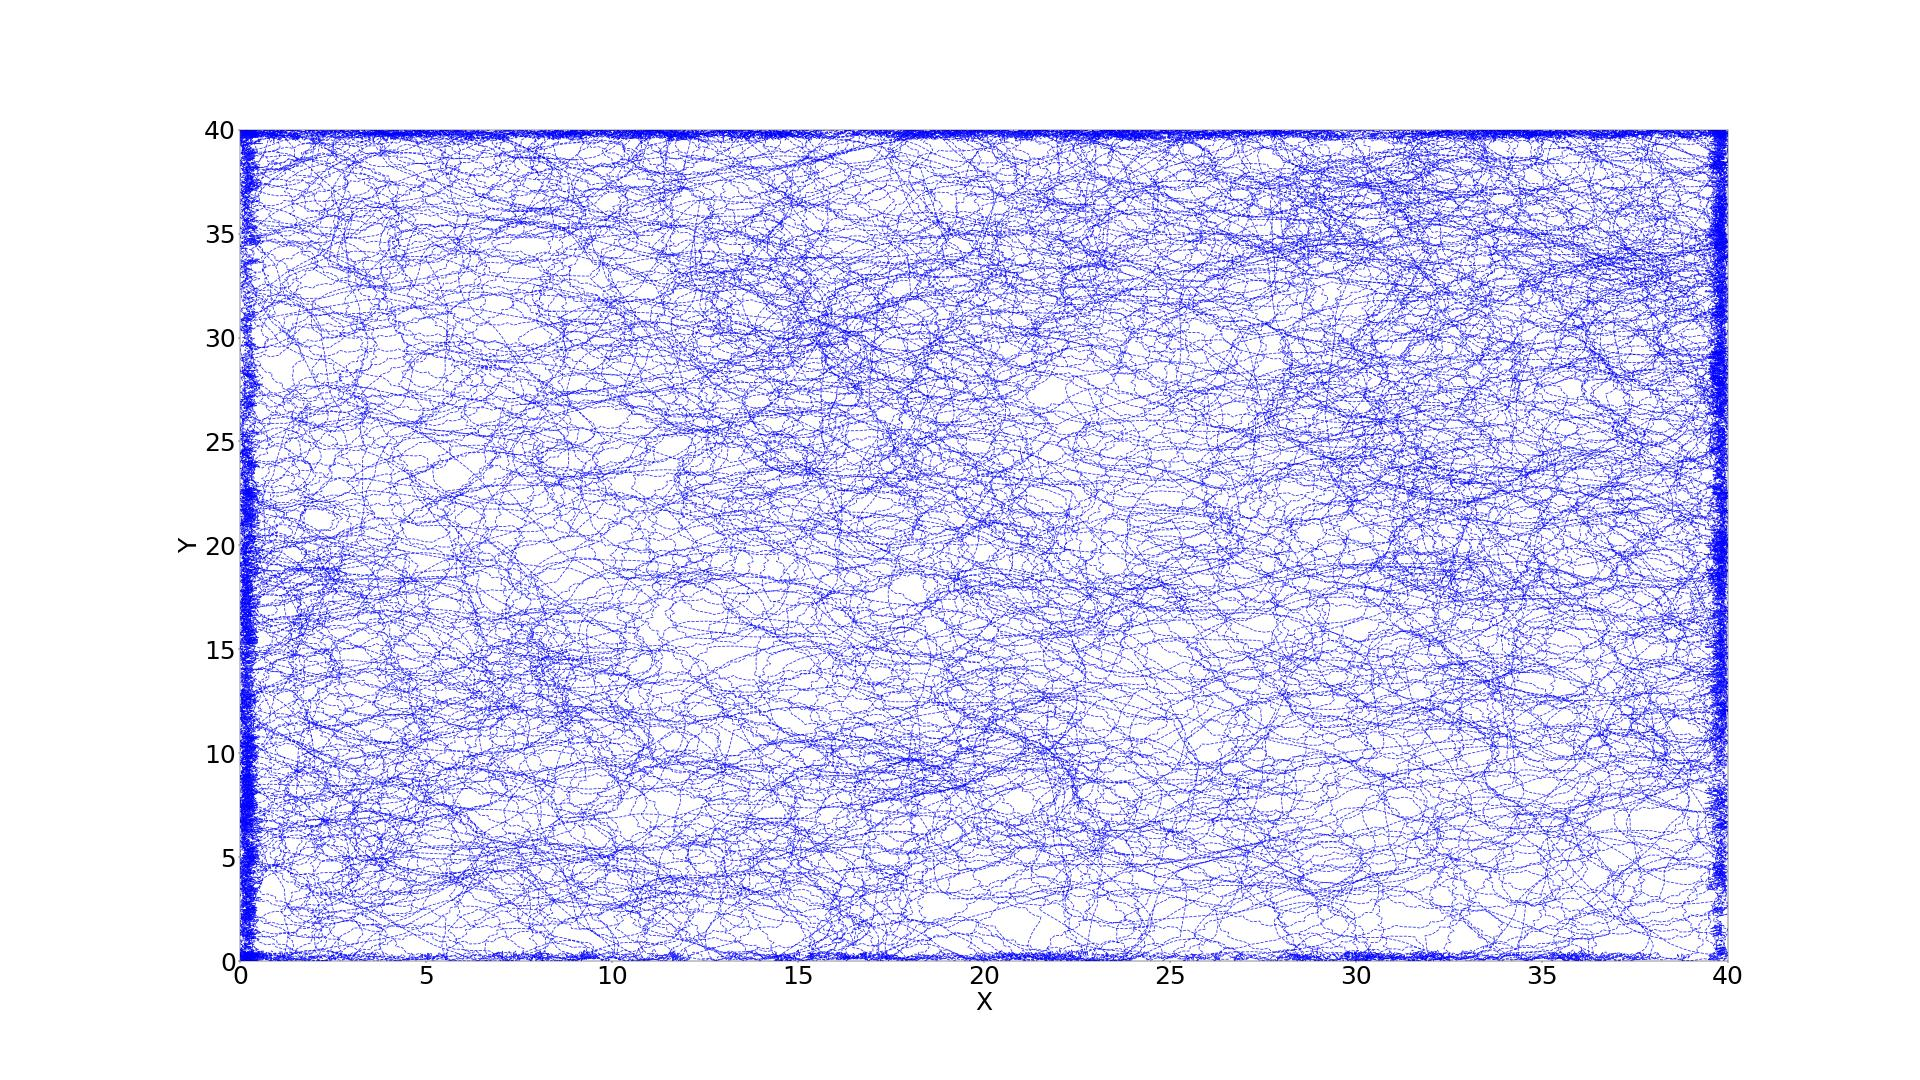
\includegraphics[width=1\linewidth]{LateX images/log/q/g1-1.6}
	\caption{Διάγραμμα διαδρομής ρομποτικού συστήματος για, $k = 0.9$ και $q = -1.6$.}
	\label{f:g68}	
\end{figure}

\clearpage

Στο Σχ. \ref{f:g69} παρατίθεται το διάγραμμα κίνησης του συστήματος, για $k=0.9$ , και $q = -1.9$. Για την επιλεγμένη τιμή της παραμέτρου \emph{q} το σύστημα διακριτού χρόνου χαρακτηρίζεται επίσης από χαοτική συμπεριφορά.

Το ποσοστό κάλυψης του χώρου για $q = -1.9$ και για δεδομένες τιμές των υπολοίπων παραμέτρων είναι $79.22 \%$. Το ποσοστό αυτό είναι σχέτικα ικανοποιητικό , διότι το ρομπότ θα μπορέσει να καλύψει ένα μεγάλο μέρος της επιφάνειας στην οποία του ζητήθηκε να κινηθεί, κάτι που παρατηρούμε στο \ref{f:g69}.


\begin{figure}[ht]
	\centering
	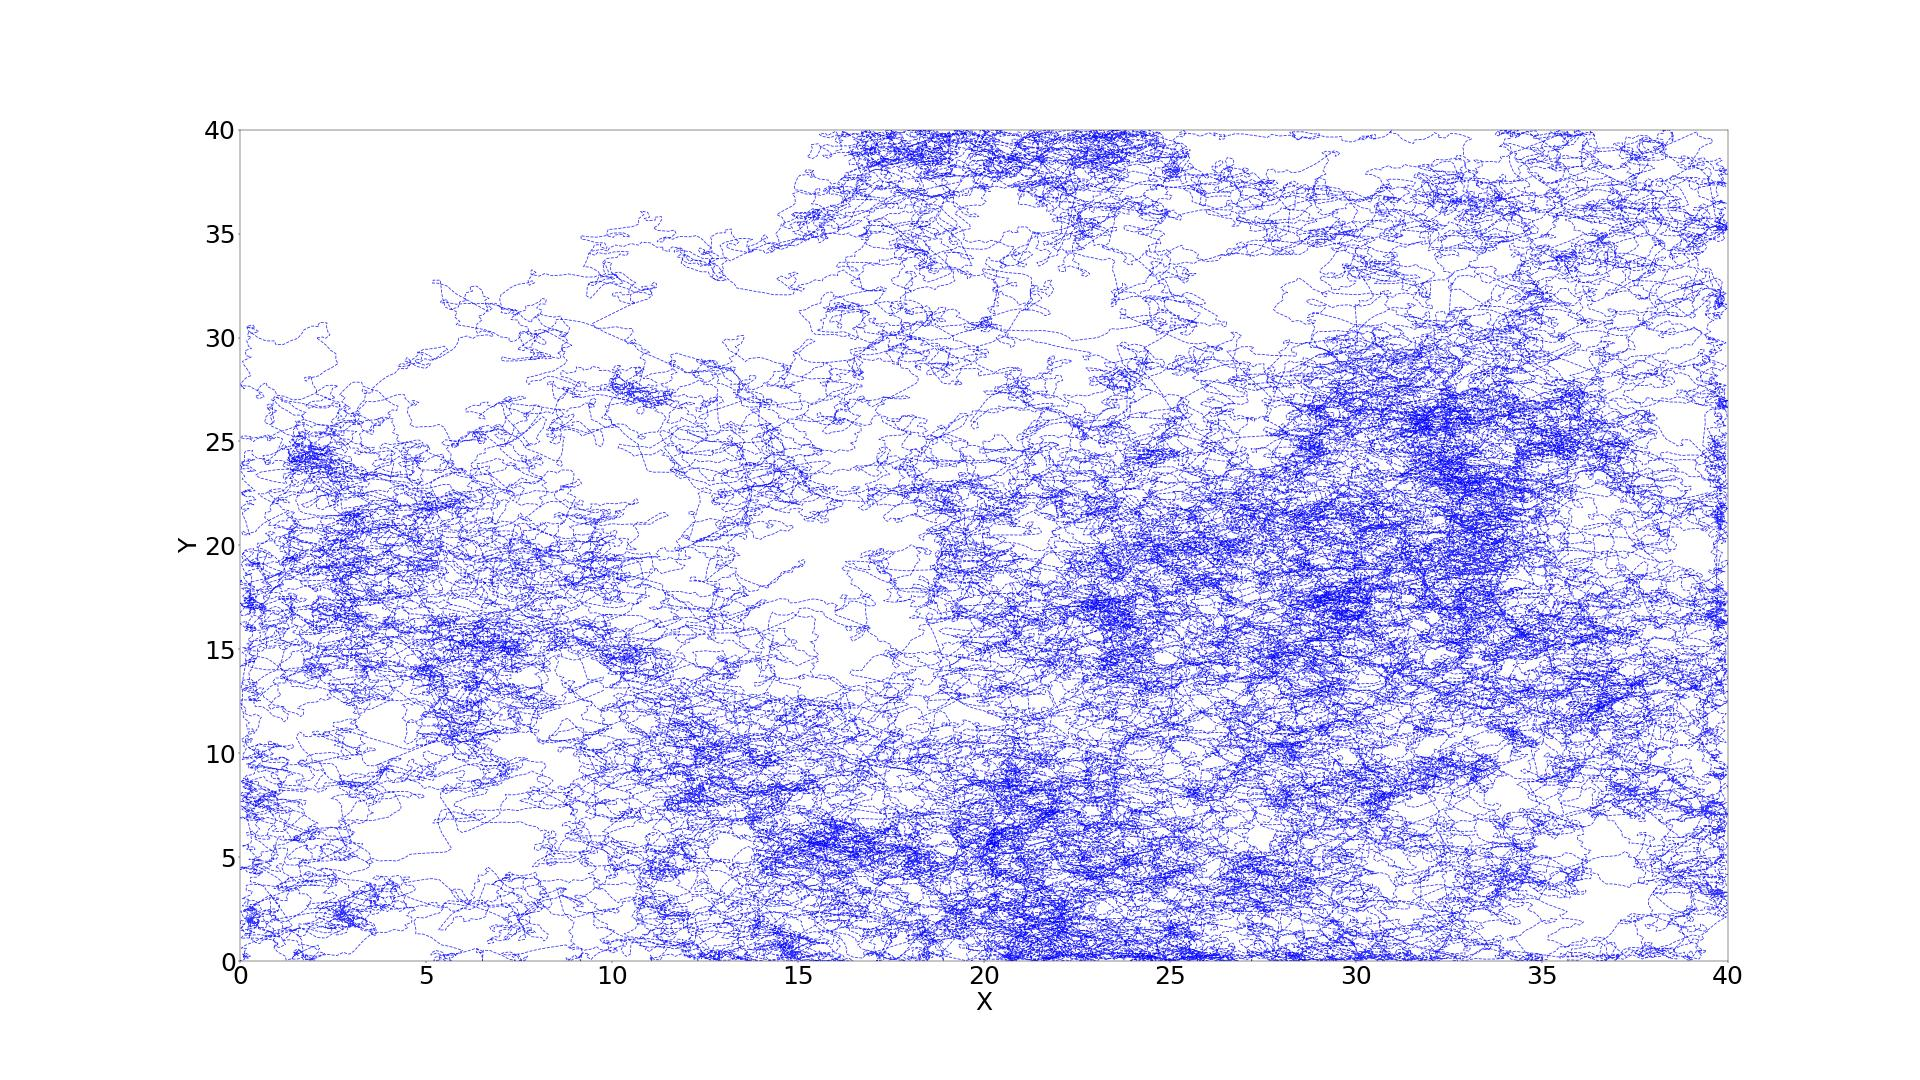
\includegraphics[width=1\linewidth]{LateX images/log/q/g1-1.9}
	\caption{Διάγραμμα διαδρομής ρομποτικού συστήματος για, $k = 0.9$ και $q = -1.9$.}
	\label{f:g69}	
\end{figure}


Στο Σχ. \ref{f:g70} παρατίθεται το διάγραμμα κίνησης του συστήματος, για $k=0.9$ , και $q = -2.1$. Για την επιλεγμένη τιμή της παραμέτρου \emph{q} το σύστημα διακριτού χρόνου χαρακτηρίζεται επίσης από χαοτική συμπεριφορά.


Στο Σχ. \ref{f:g71} παρουσιάζονται σε κοινό διάγραμμα οι κινήσεις του συστήματος, για τις
περιπτώσεις που παρουσιάστηκαν παραπάνω, δηλαδή για $k=0.9$ , και $q = -1.6$ \emph{(μπλέ χρώμα)}
$q = -1.9$ \emph{(κόκκινο χρώμα)}.

\begin{figure}[ht]
	\centering
	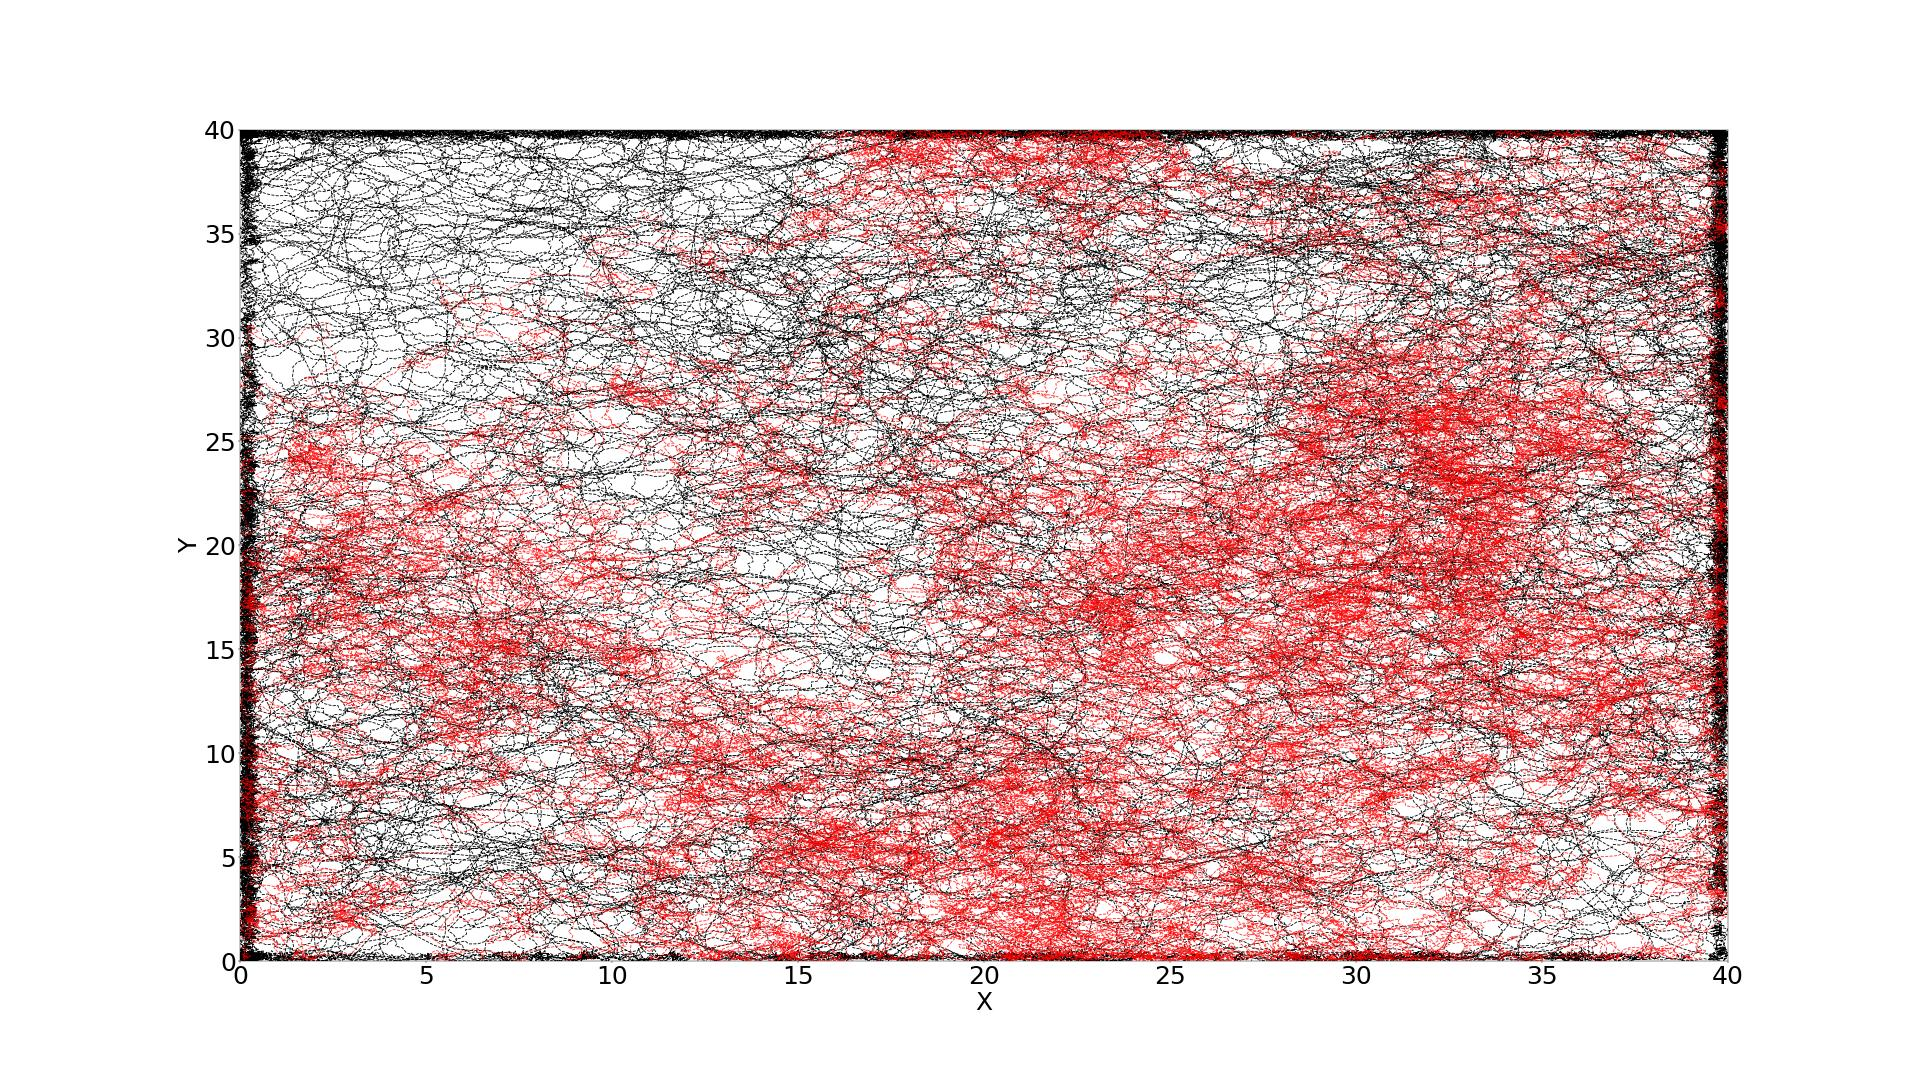
\includegraphics[width=1\linewidth]{LateX images/log/q/g1}
	\caption{Κοινό διάγραμμα διαδρομής ρομποτικού συστήματος για, $k = 0.9$ , $q = -1.6$ \emph{(μπλέ χρώμα)}, $q = -1.9$ \emph{(κόκκινο χρώμα)}.}
	\label{f:g71}	
\end{figure}

Από το Σχ. \ref{f:g71} είναι δυνατή η σύγκριση των τριών κινήσεων και εύκολα εξάγεται το
συμπέρασμα ότι το ρομπότ κινείται πιο αποτελεσματικά για $q = -1.6$, ενώ και για $q = -1.9$ καλύπτει αρκετά καλά την επιφάνεια που του δόθηκε.


\clearpage

\subsection{Για \emph{q = -1.4 , q = -1.6}}
\label{par:g1}
Στην παράγραφο αυτή θα μελετηθεί ο τρόπος συμπεριφοράς του ρομποτικού συστήματος όταν μεταβάλλεται η παράμετρος \emph{q} και η παράμετρος \emph{k} παραμένει σταθερή.

Στο Σχ. \ref{f:g72} παρατίθεται το διάγραμμα κίνησης του συστήματος, για $k=0.79$ , και $q = -1.4$. Για την επιλεγμένη τιμή της παραμέτρου \emph{q} το σύστημα διακριτού χρόνου χαρακτηρίζεται επίσης από χαοτική συμπεριφορά.

Το ποσοστό κάλυψης του χώρου για $q = -1.4$ και για δεδομένες τιμές των υπολοίπων παραμέτρων είναι $87.04 \%$. Το ποσοστό αυτό είναι σχέτικα ικανοποιητικό , διότι το ρομπότ θα μπορέσει να καλύψει ένα μεγάλο μέρος της επιφάνειας στην οποία του ζητήθηκε να κινηθεί, κάτι που παρατηρούμε στο \ref{f:g72}.


\begin{figure}[ht]
	\centering
	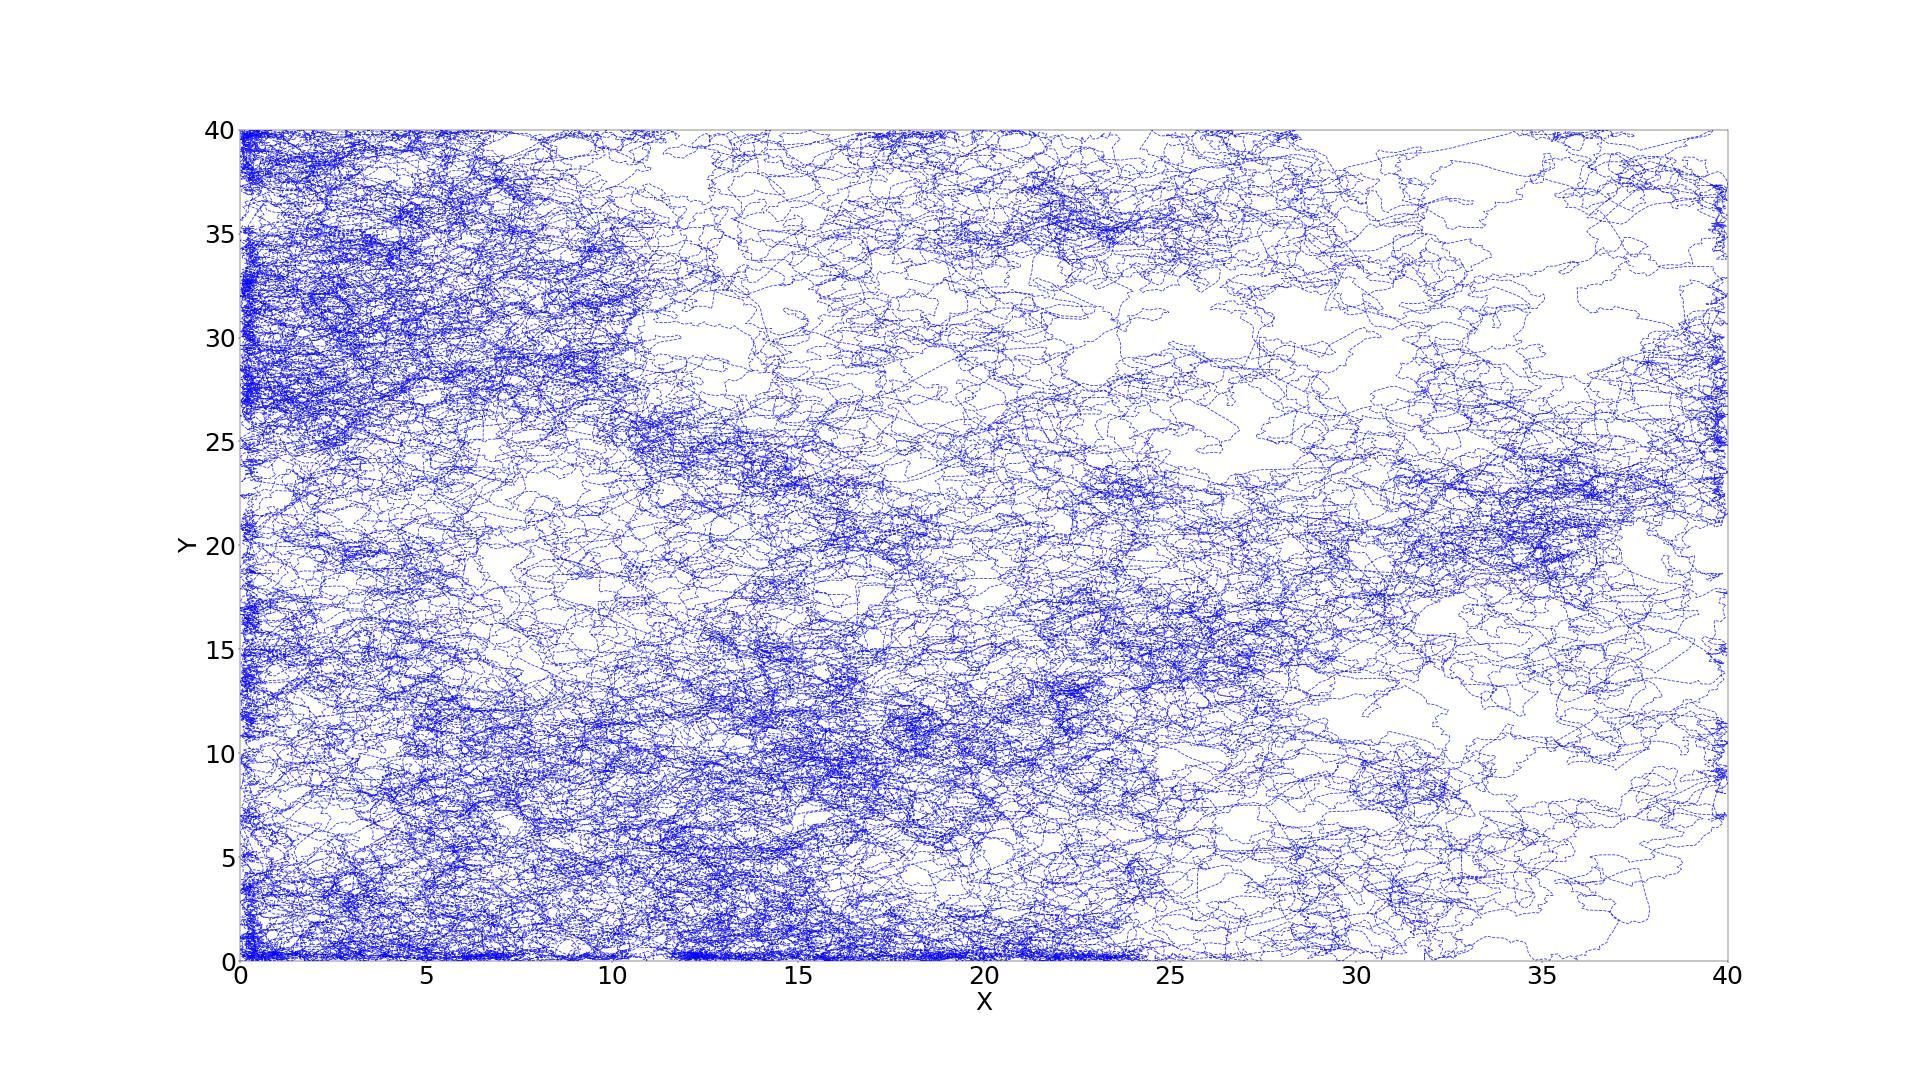
\includegraphics[width=1\linewidth]{LateX images/log/q/g3-1.4}
	\caption{Διάγραμμα διαδρομής ρομποτικού συστήματος για, $k = 0.79$ και $q = -1.4$.}
	\label{f:g72}	
\end{figure}

Στο Σχ. \ref{f:g73} παρατίθεται το διάγραμμα κίνησης του συστήματος, για $k=0.79$ , και $q = -1.6$. Για την παράμετρο διακλάδωσης \emph{k} επιλέγονται τιμές για τις οποίες το σύστημα διακριτού χρόνου χαρακτηρίζεται από χαοτική συμπεριφορά.

Για την παραπάνω κίνηση υπολογίστηκε ότι το ποσοστό κάλυψης του χώρου είναι
$9.6 \% $. Το ποσοστό αυτό επιβεβαιώνει το διάγραμμα \ref{f:g73}, δηλαδή το ρομπότ στην συγκεκριμένη περίπτωση καλύπτει ένα πολύ μικρό μέρος της επιφάνειας που του δόθηκε.

\begin{figure}[ht]
	\centering
	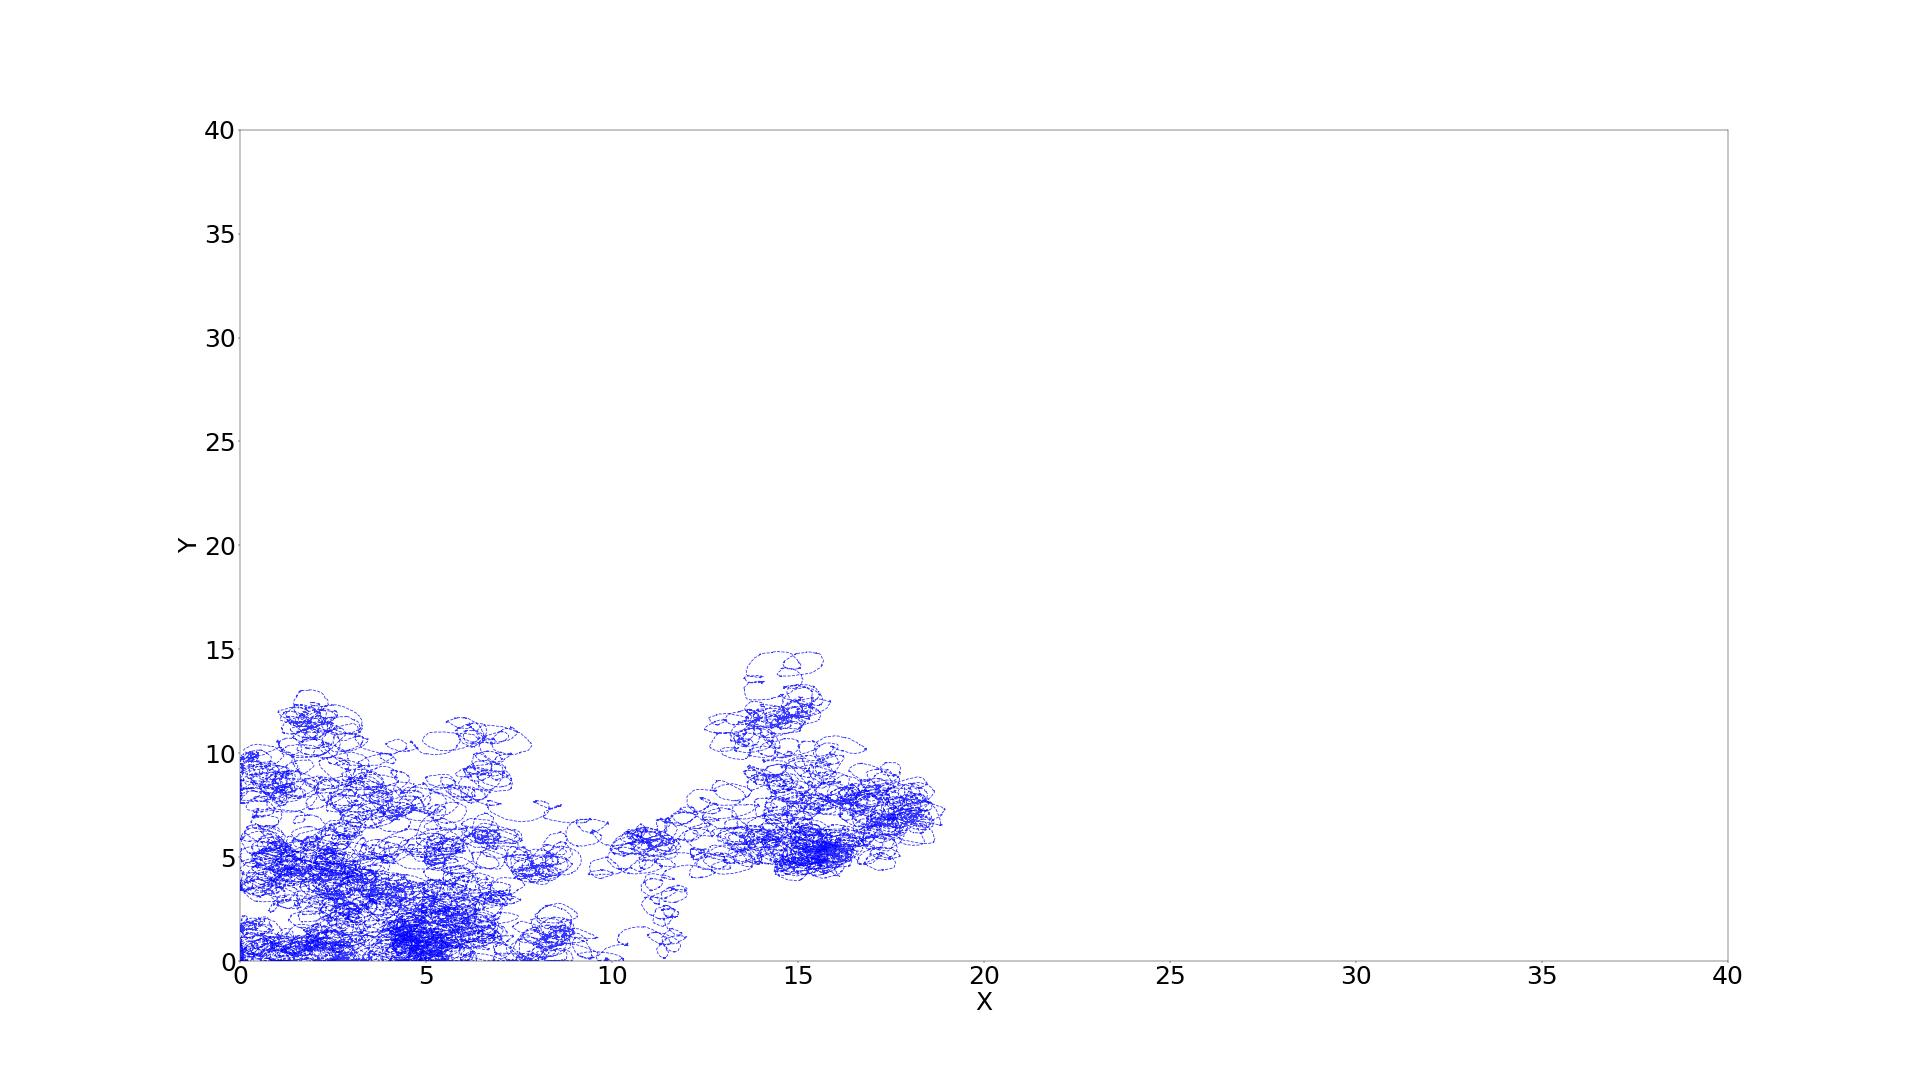
\includegraphics[width=1\linewidth]{LateX images/log/q/g3-1.6}
	\caption{Διάγραμμα διαδρομής ρομποτικού συστήματος για, $k = 0.79$ και $q = -1.6$.}
	\label{f:g73}	
\end{figure}


Στο Σχ. \ref{f:g74} παρουσιάζονται σε κοινό διάγραμμα οι κινήσεις του συστήματος, για τις
περιπτώσεις που παρουσιάστηκαν παραπάνω, δηλαδή για $k=0.79$ , και $q = -1.4$ \emph{(μαύρο χρώμα)}, $q = -1.6$  \emph{(κόκκινο χρώμα)}.

\begin{figure}[ht]
	\centering
	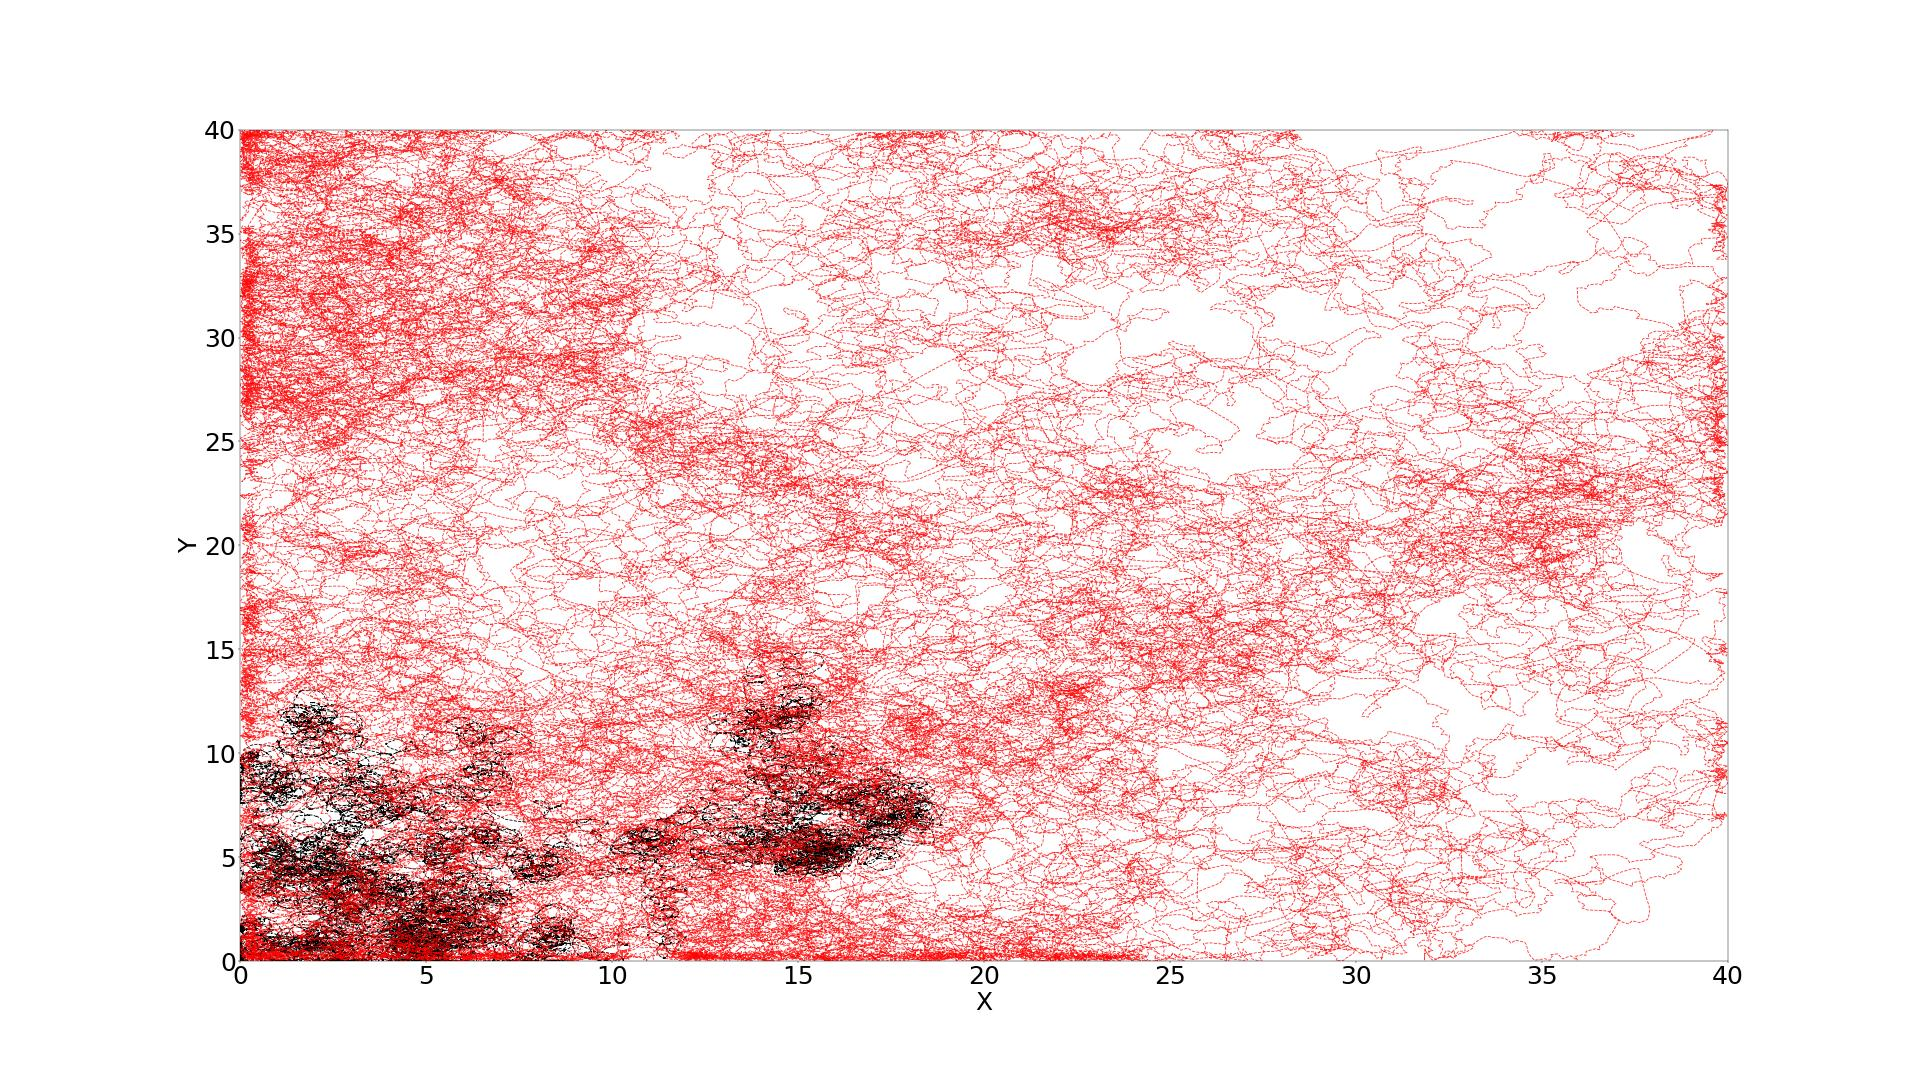
\includegraphics[width=1\linewidth]{LateX images/log/q/g3}
	\caption{Κοινό διάγραμμα διαδρομής ρομποτικού συστήματος για, $k = 0.79$ , $q = -1.4$ \emph{(μαύρο χρώμα)}, $q = -1.6$  \emph{(κόκκινο χρώμα)}.}
	\label{f:g74}	
\end{figure}

Από το Σχ. \ref{f:g74} είναι δυνατή η σύγκριση των δύο κινήσεων και εύκολα εξάγεται το
συμπέρασμα ότι το ρομπότ κινείται πιο αποτελεσματικά για $q = -1.4$.

\clearpage

\subsection{Για \emph{q = -1.9 , q = -2.1}}

Στην παράγραφο αυτή θα μελετηθεί ο τρόπος συμπεριφοράς του ρομποτικού συστήματος όταν μεταβάλλεται η παράμετρος \emph{q} και η παράμετρος \emph{k} παραμένει σταθερή.

Στο Σχ. \ref{f:g75} παρατίθεται το διάγραμμα κίνησης του συστήματος, για $k=0.68$ , και $q = -1.9$. Για την επιλεγμένη τιμή της παραμέτρου \emph{q} το σύστημα διακριτού χρόνου χαρακτηρίζεται επίσης από χαοτική συμπεριφορά.

Το ποσοστό κάλυψης του χώρου για $q = -1.9$ και για δεδομένες τιμές των υπολοίπων παραμέτρων είναι $85.78 \%$. Το ποσοστό αυτό είναι σχέτικα ικανοποιητικό , διότι το ρομπότ θα μπορέσει να καλύψει ένα μεγάλο μέρος της επιφάνειας στην οποία του ζητήθηκε να κινηθεί, κάτι που παρατηρούμε στο \ref{f:g75}.


\begin{figure}[ht]
	\centering
	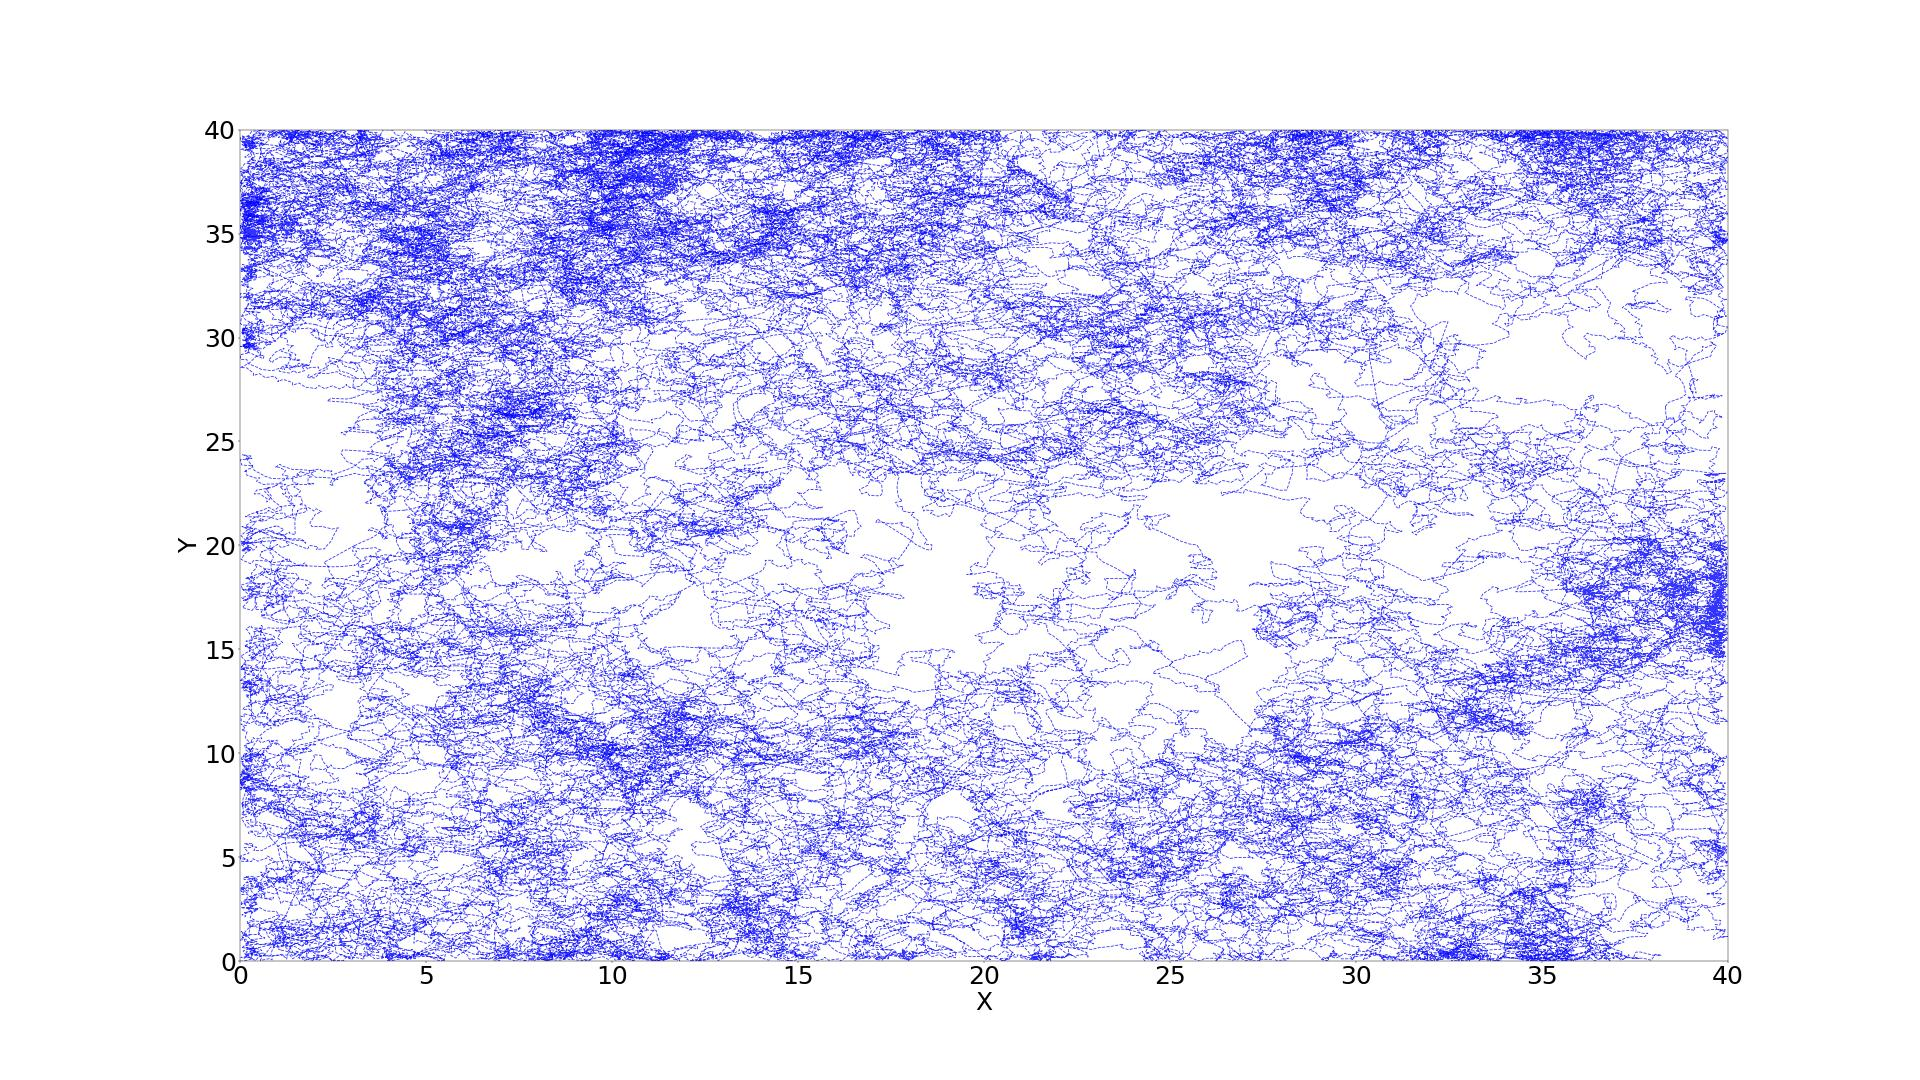
\includegraphics[width=1\linewidth]{LateX images/log/q/g2-1.9}
	\caption{Διάγραμμα διαδρομής ρομποτικού συστήματος για, $k = 0.68$ και $q = -1.9$.}
	\label{f:g75}	
\end{figure}

Στο Σχ. \ref{f:g76} παρατίθεται το διάγραμμα κίνησης του συστήματος, για $k=0.68$ , και $q = -1.9$. Για την παράμετρο διακλάδωσης \emph{k} επιλέγονται τιμές για τις οποίες το σύστημα διακριτού χρόνου χαρακτηρίζεται από χαοτική συμπεριφορά.

Για την παραπάνω κίνηση υπολογίστηκε ότι το ποσοστό κάλυψης του χώρου είναι
$54.121 \% $. Το ποσοστό αυτό είναι μας δείχνει οτι το ρομπότ καλύπτει λίγο παραπάνω απο το μισό της επιφάνειας που του ζητήθηκε να κινηθεί  , κάτι που παρατηρούμε στο \ref{f:g76}

\begin{figure}[ht]
	\centering
	\includegraphics[width=1\linewidth]{LateX images/log/q/g2-2.1}
	\caption{Διάγραμμα διαδρομής ρομποτικού συστήματος για, $k = 0.68$ και $q = -2.1$.}
	\label{f:g76}	
\end{figure}


Στο Σχ. \ref{f:g77} παρουσιάζονται σε κοινό διάγραμμα οι κινήσεις του συστήματος, για τις
περιπτώσεις που παρουσιάστηκαν παραπάνω, δηλαδή για $k=0.68$ , και $q = -1.9$ \emph{(μαύρο χρώμα)}, $q = -2.1$  \emph{(κόκκινο χρώμα)}.

\begin{figure}[ht]
	\centering
	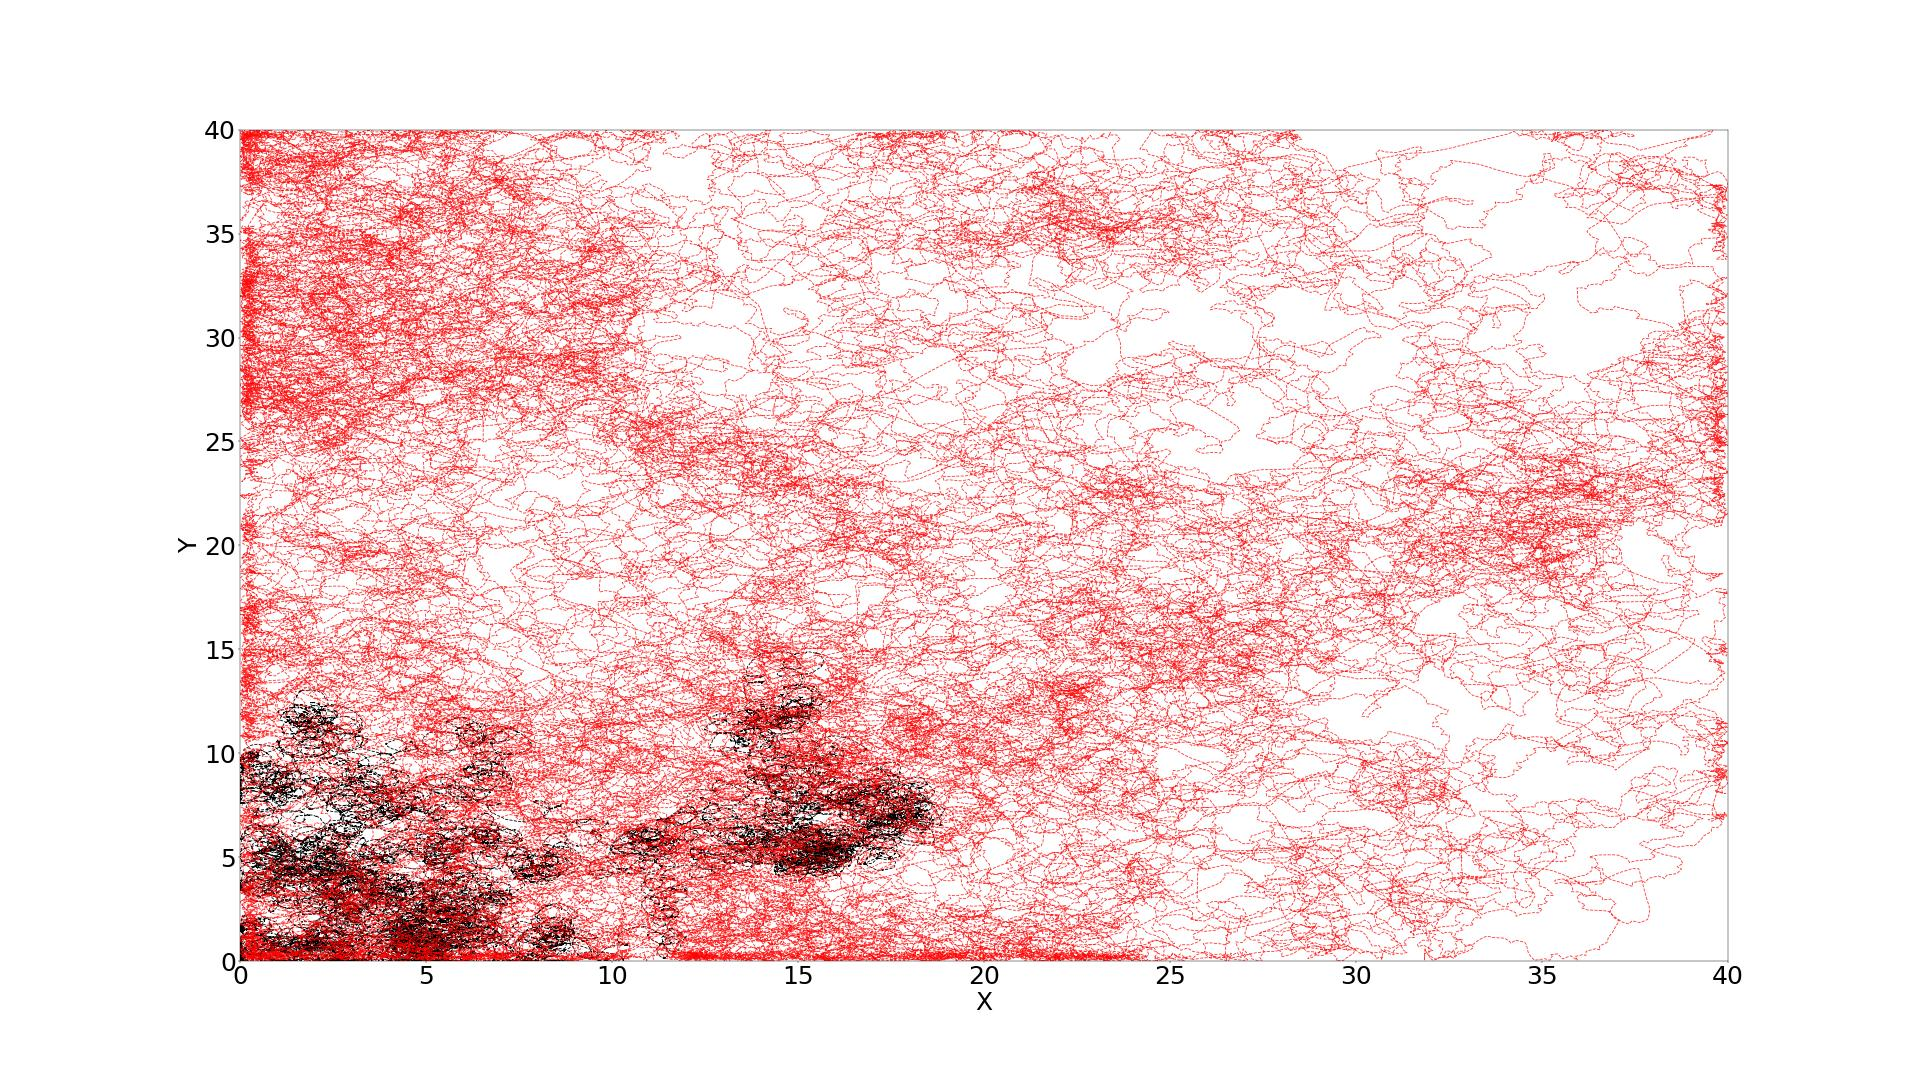
\includegraphics[width=1\linewidth]{LateX images/log/q/g3}
	\caption{Κοινό διάγραμμα διαδρομής ρομποτικού συστήματος για, $k = 0.68$ , $q = -1.9$ \emph{(μαύρο χρώμα)}, $q = -2.1$  \emph{(κόκκινο χρώμα)}.}
	\label{f:g77}	
\end{figure}

Από το Σχ. \ref{f:g77} είναι δυνατή η σύγκριση των δύο κινήσεων και εύκολα εξάγεται το
συμπέρασμα ότι το ρομπότ κινείται πιο αποτελεσματικά για $q = -1.9$.

\clearpage

\subsection{Για \emph{k = 0.68 , k = 0.69 , k = 0.815}}
\label{par:g2}
Στην παράγραφο αυτή θα μελετηθεί ο τρόπος συμπεριφοράς του ρομποτικού συστήματος όταν μεταβάλλεται η παράμετρος \emph{κ} και η παράμετρος \emph{q} παραμένει σταθερή. Θα αναλυθεί η περίπτωση όπου το $ q =-1.6$ ενώ πέρα απο τα $k = 0.68 , k = 0.69 , k = 0.815$ θα συγκρίνουμε και τις άλλες δύο τιμές του \emph{k} οι οποίες προέκυψαν στις προηγούμενες παραγράφους.

Στο Σχ. \ref{f:g78} παρατίθεται το διάγραμμα κίνησης του συστήματος, για, $q = -1.6$ και $k = 0.68$.
Το ποσοστό κάλυψης του χώρου είναι  $5.4 \%$. 

Στο Σχ.\ref{f:g79} παρατίθεται το διάγραμμα κίνησης του συστήματος, για, $q = -1.6$ και $k = 0.69$.
Το ποσοστό κάλυψης του χώρου είναι  $6.72 \%$.

Στο Σχ. \ref{f:g80} παρατίθεται το διάγραμμα κίνησης του συστήματος, για, $q = -1.6$ και $k = 0.815$.
Το ποσοστό κάλυψης του χώρου είναι  $95.7\%$.

Σε σύγκριση με τα Σχ. \ref{f:g68} και \ref{f:g73} οι παράμετροι του \emph{k} για $q = -1.6$ που παρουσιάζονται στα Σχ. \ref{f:g78} και \ref{f:g79} έχουν μικρότερη καλυψιμότητα, ειδικά σε σχέση με το 
Σχ. \ref{f:g68} όπου το ποσοστό αγγίζει το $95.78\%$.

Από την άλλη η παράμετρος του \emph{k} για $q = -1.6$ του Σχ. \ref{f:g80} ξεπερνάει όλές τις προηγούμενες παραμέτρους του \emph{k} σε καλυψιμότητα σε μεγάλο βαθμό, πέρα από του Σχ. \ref{f:g68} όπου το ποσοστό είναι παρόμοιο.

\begin{figure}[ht]
	\centering
	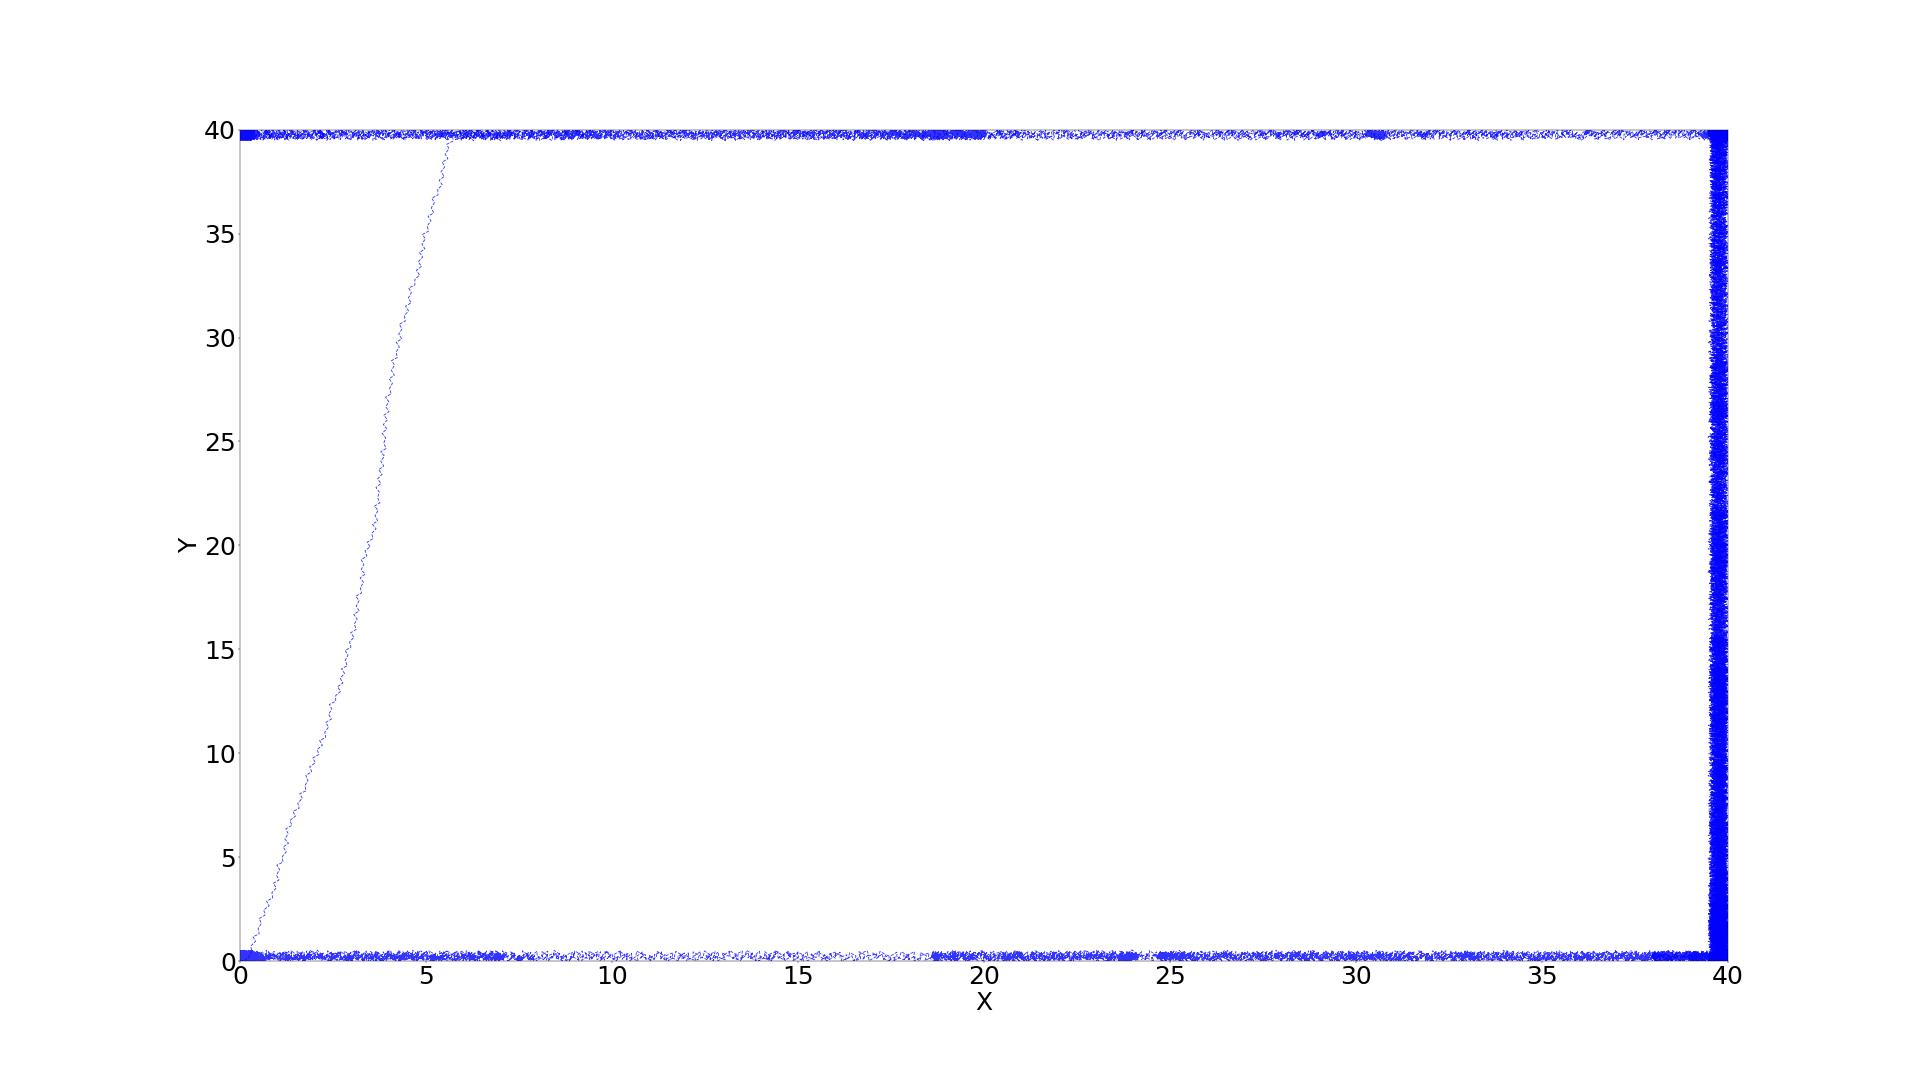
\includegraphics[width=1\linewidth]{LateX images/log/k/g1-1.6}
	\caption{Διάγραμμα διαδρομής ρομποτικού συστήματος για, $q = -1.6$ και $k = 0.68$.}
	\label{f:g78}	
\end{figure}

\begin{figure}[ht]
	\centering
	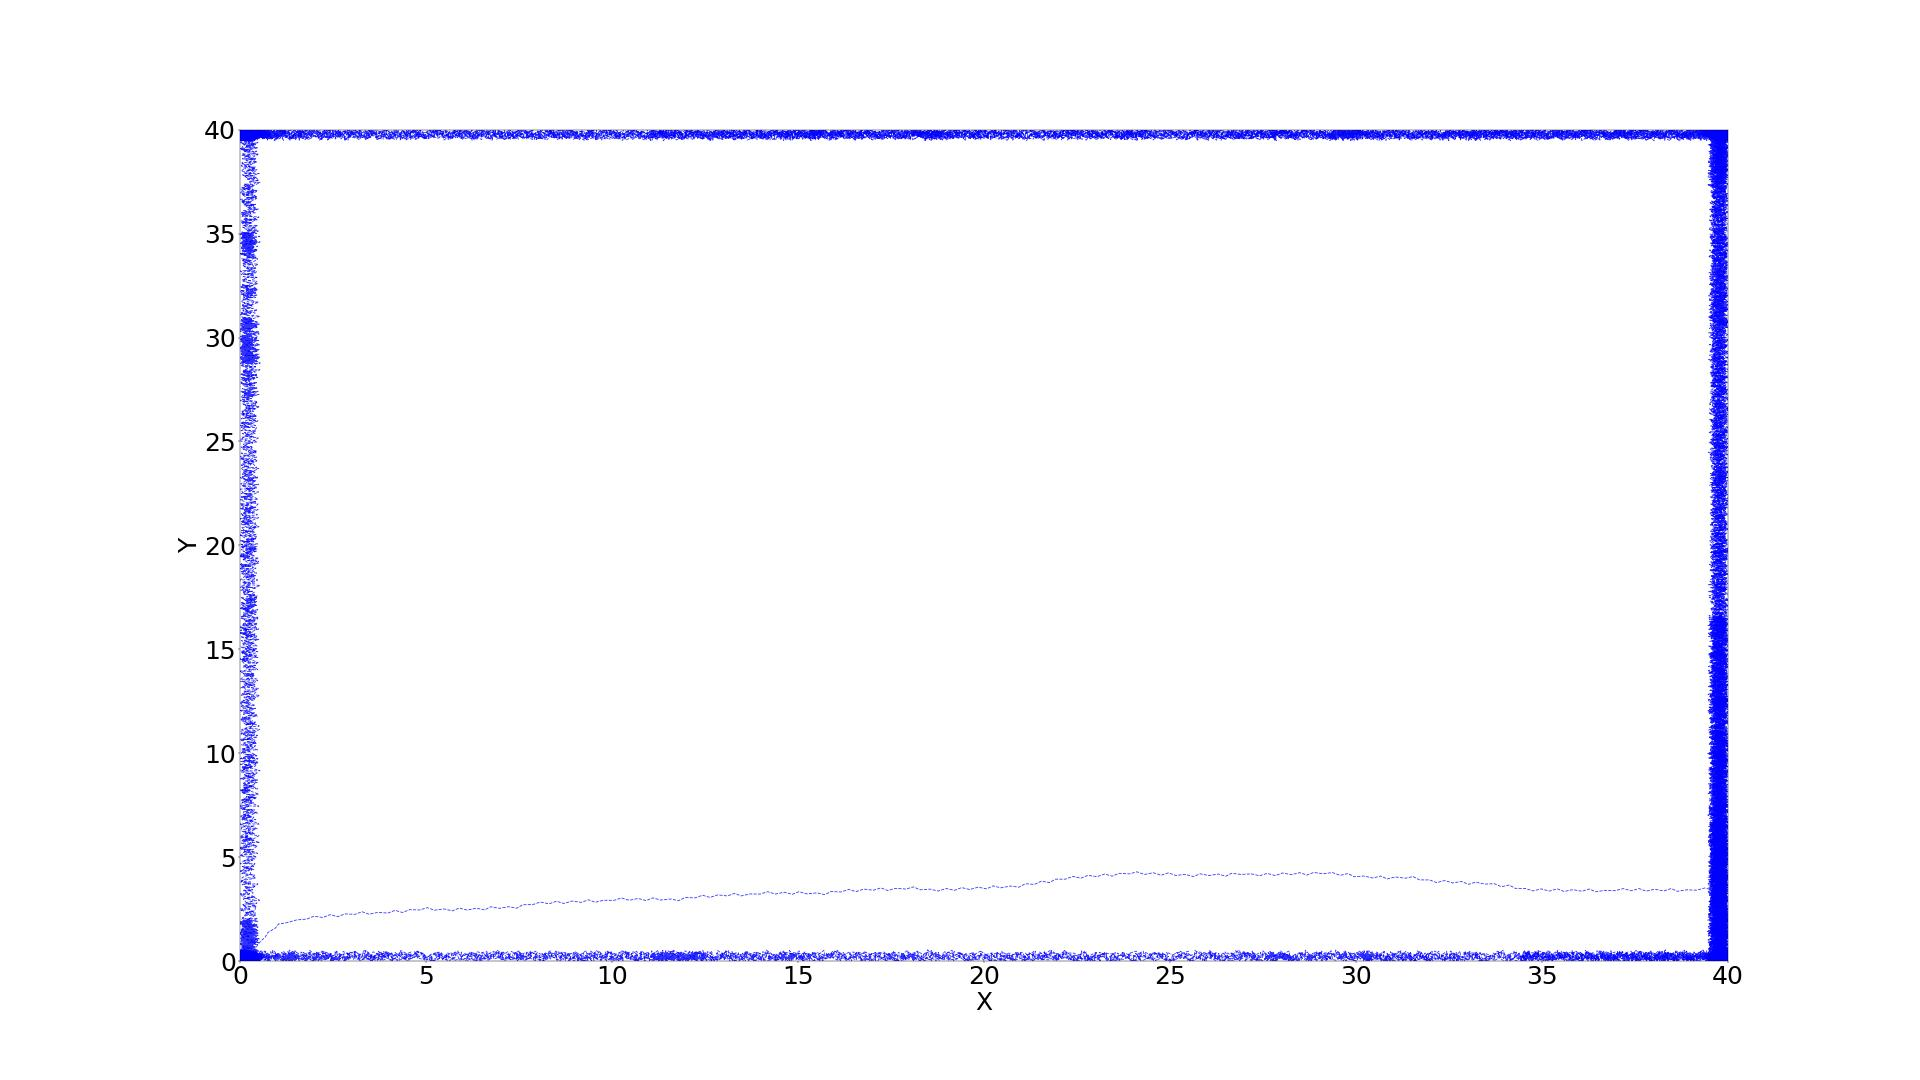
\includegraphics[width=1\linewidth]{LateX images/log/k/g2-1.6}
	\caption{Διάγραμμα διαδρομής ρομποτικού συστήματος για, $q = -1.6$ και $k = 0.69$.}
	\label{f:g79}	
\end{figure}

\begin{figure}[ht]
	\centering
	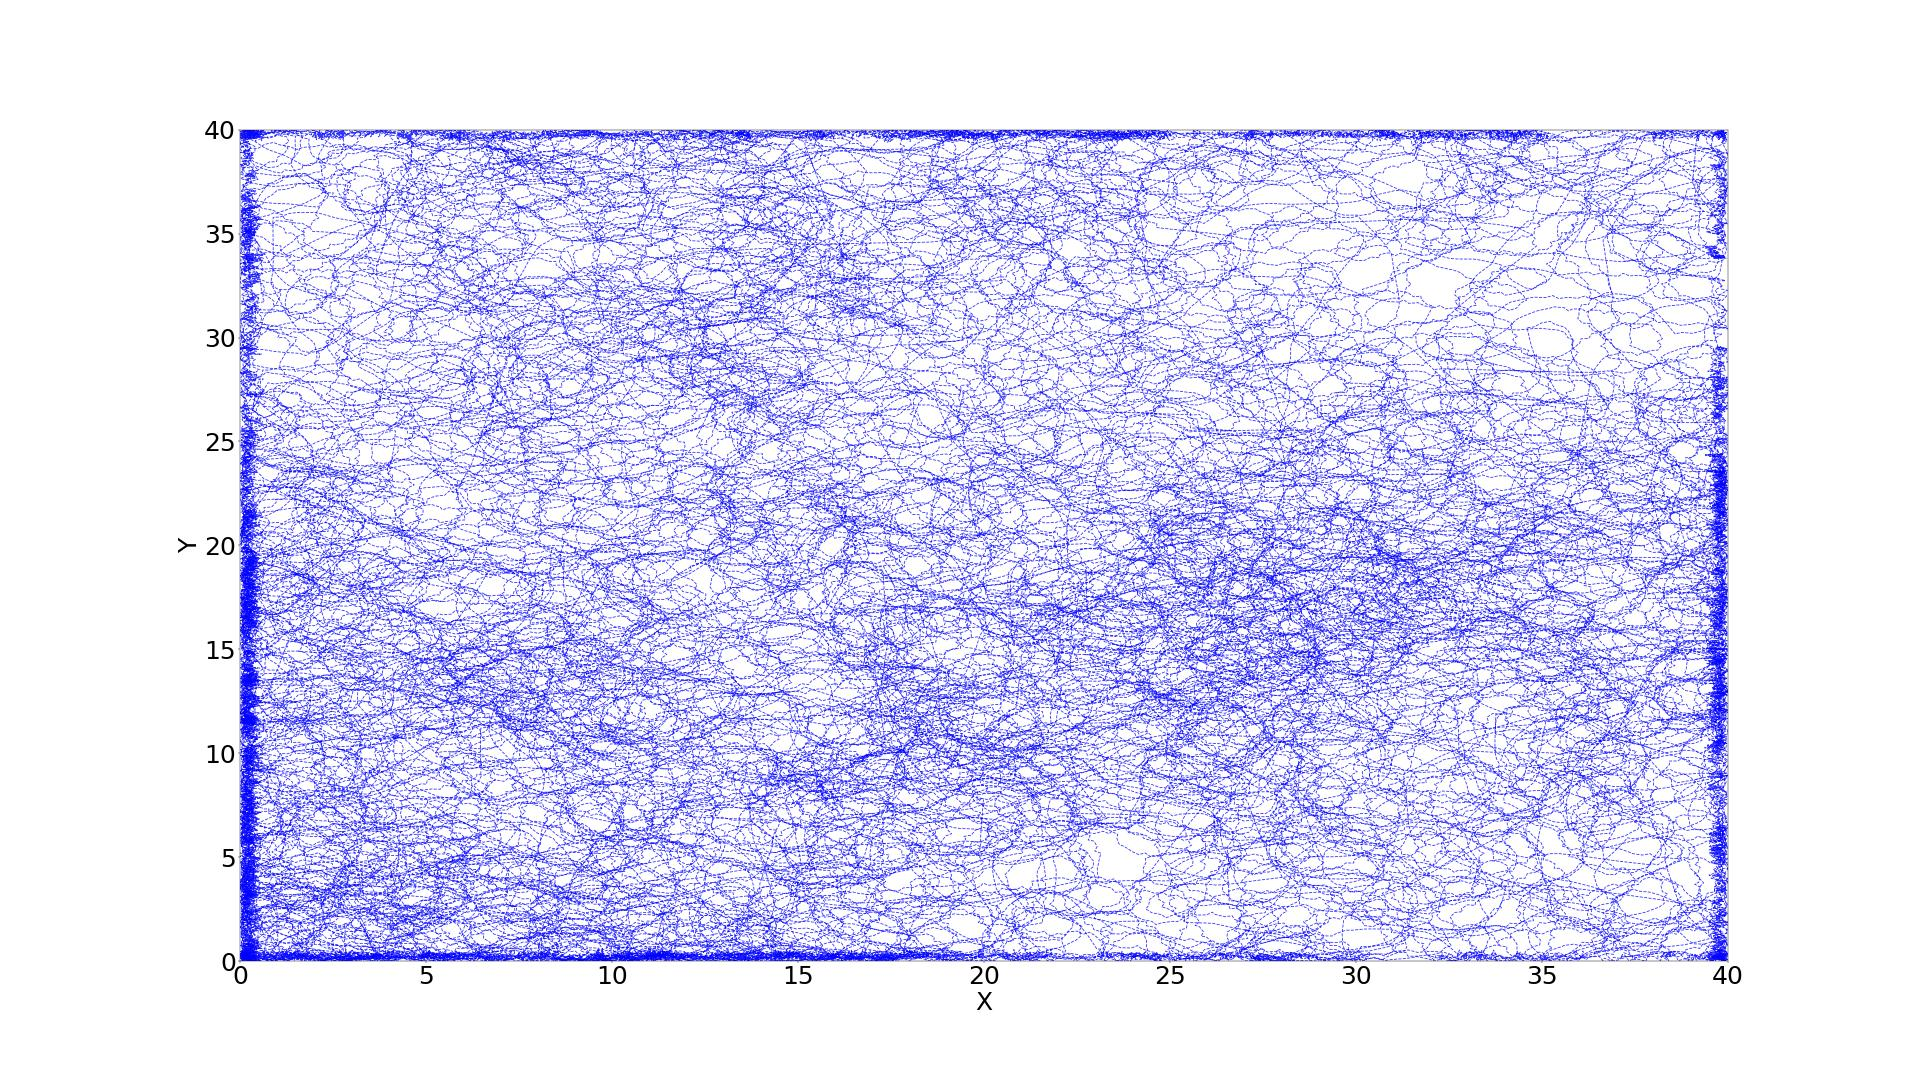
\includegraphics[width=1\linewidth]{LateX images/log/k/g3-1.6}
	\caption{Διάγραμμα διαδρομής ρομποτικού συστήματος για, $q = -1.6$ και $k = 0.815$.}
	\label{f:g80}	
\end{figure}


\clearpage

\subsection{Για \emph{k = 0.74 , k = 0.751 , k = 0.76}}
\label{par:g3}
Στην παράγραφο αυτή θα μελετηθεί ο τρόπος συμπεριφοράς του ρομποτικού συστήματος όταν μεταβάλλεται η παράμετρος \emph{κ} και η παράμετρος \emph{q} παραμένει σταθερή. Θα αναλυθεί η περίπτωση όπου το $ q =-1.4$ ενώ πέρα απο τα $k = 0.74 , k = 0.751 , k = 0.76$ θα συγκρίνουμε και την άλλη τιμή του \emph{k} που προέκυψε στην παράγραφο \ref{par:g1}.

Στο Σχ. \ref{f:g81} παρατίθεται το διάγραμμα κίνησης του συστήματος, για, $q = -1.4$ και $k = 0.74$.
Το ποσοστό κάλυψης του χώρου είναι  $7.23\%$. 

Στο Σχ.\ref{f:g82} παρατίθεται το διάγραμμα κίνησης του συστήματος, για, $q = -1.4$ και $k = 0.751$.
Το ποσοστό κάλυψης του χώρου είναι  $69.95 \%$.

Στο Σχ. \ref{f:g83} παρατίθεται το διάγραμμα κίνησης του συστήματος, για, $q = -1.4$ και $k = 0.76$.
Το ποσοστό κάλυψης του χώρου είναι  $84.7\%$.

Σε σύγκριση με τo Σχ. \ref{f:g72}  οι παράμετροι του \emph{k} για $q = -1.4$ που παρουσιάζονται στα Σχ. \ref{f:g81}, \ref{f:g82} και \ref{f:g83} έχουν μικρότερη καλυψιμότητα, ειδικά το Σχ. \ref{f:g81}.

\begin{figure}[ht]
	\centering
	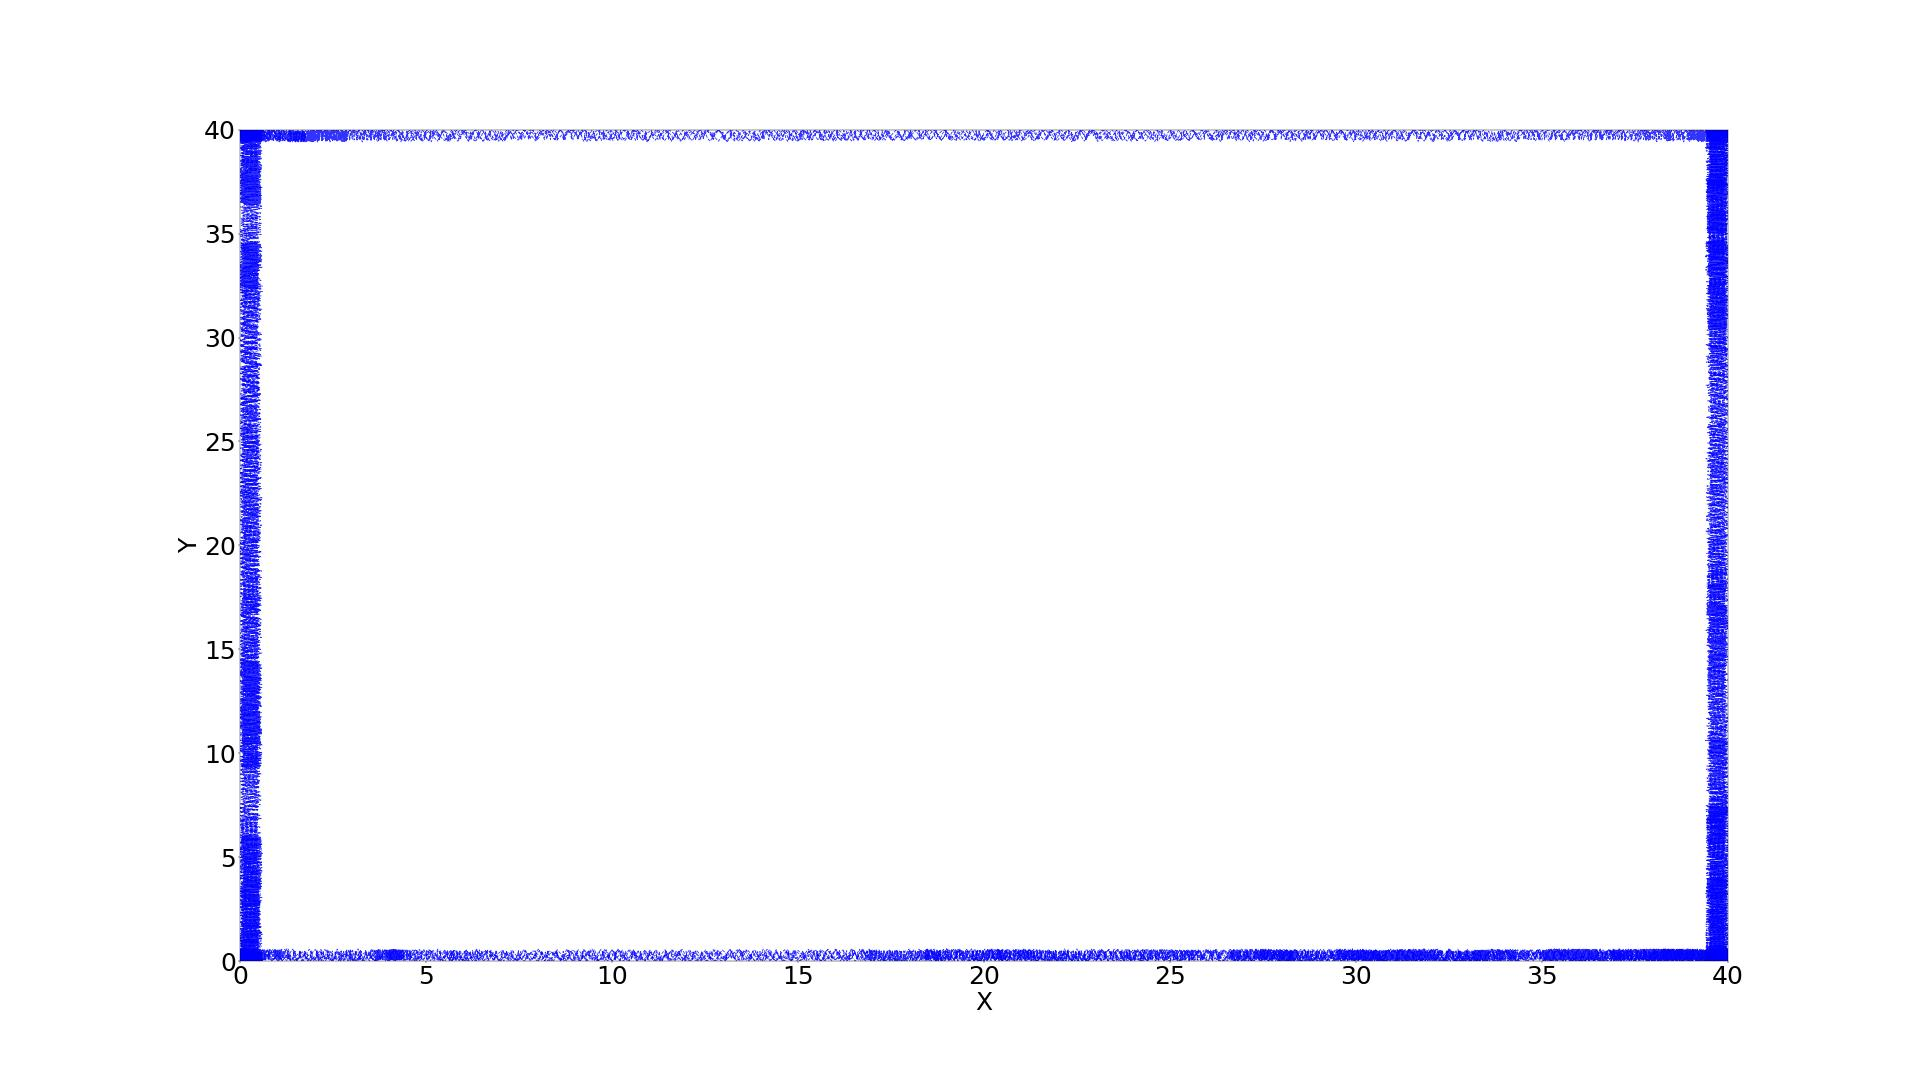
\includegraphics[width=1\linewidth]{LateX images/log/k/g1-1.4}
	\caption{Διάγραμμα διαδρομής ρομποτικού συστήματος για, $q = -1.4$ και $k = 0.74$.}
	\label{f:g81}	
\end{figure}

\begin{figure}[ht]
	\centering
	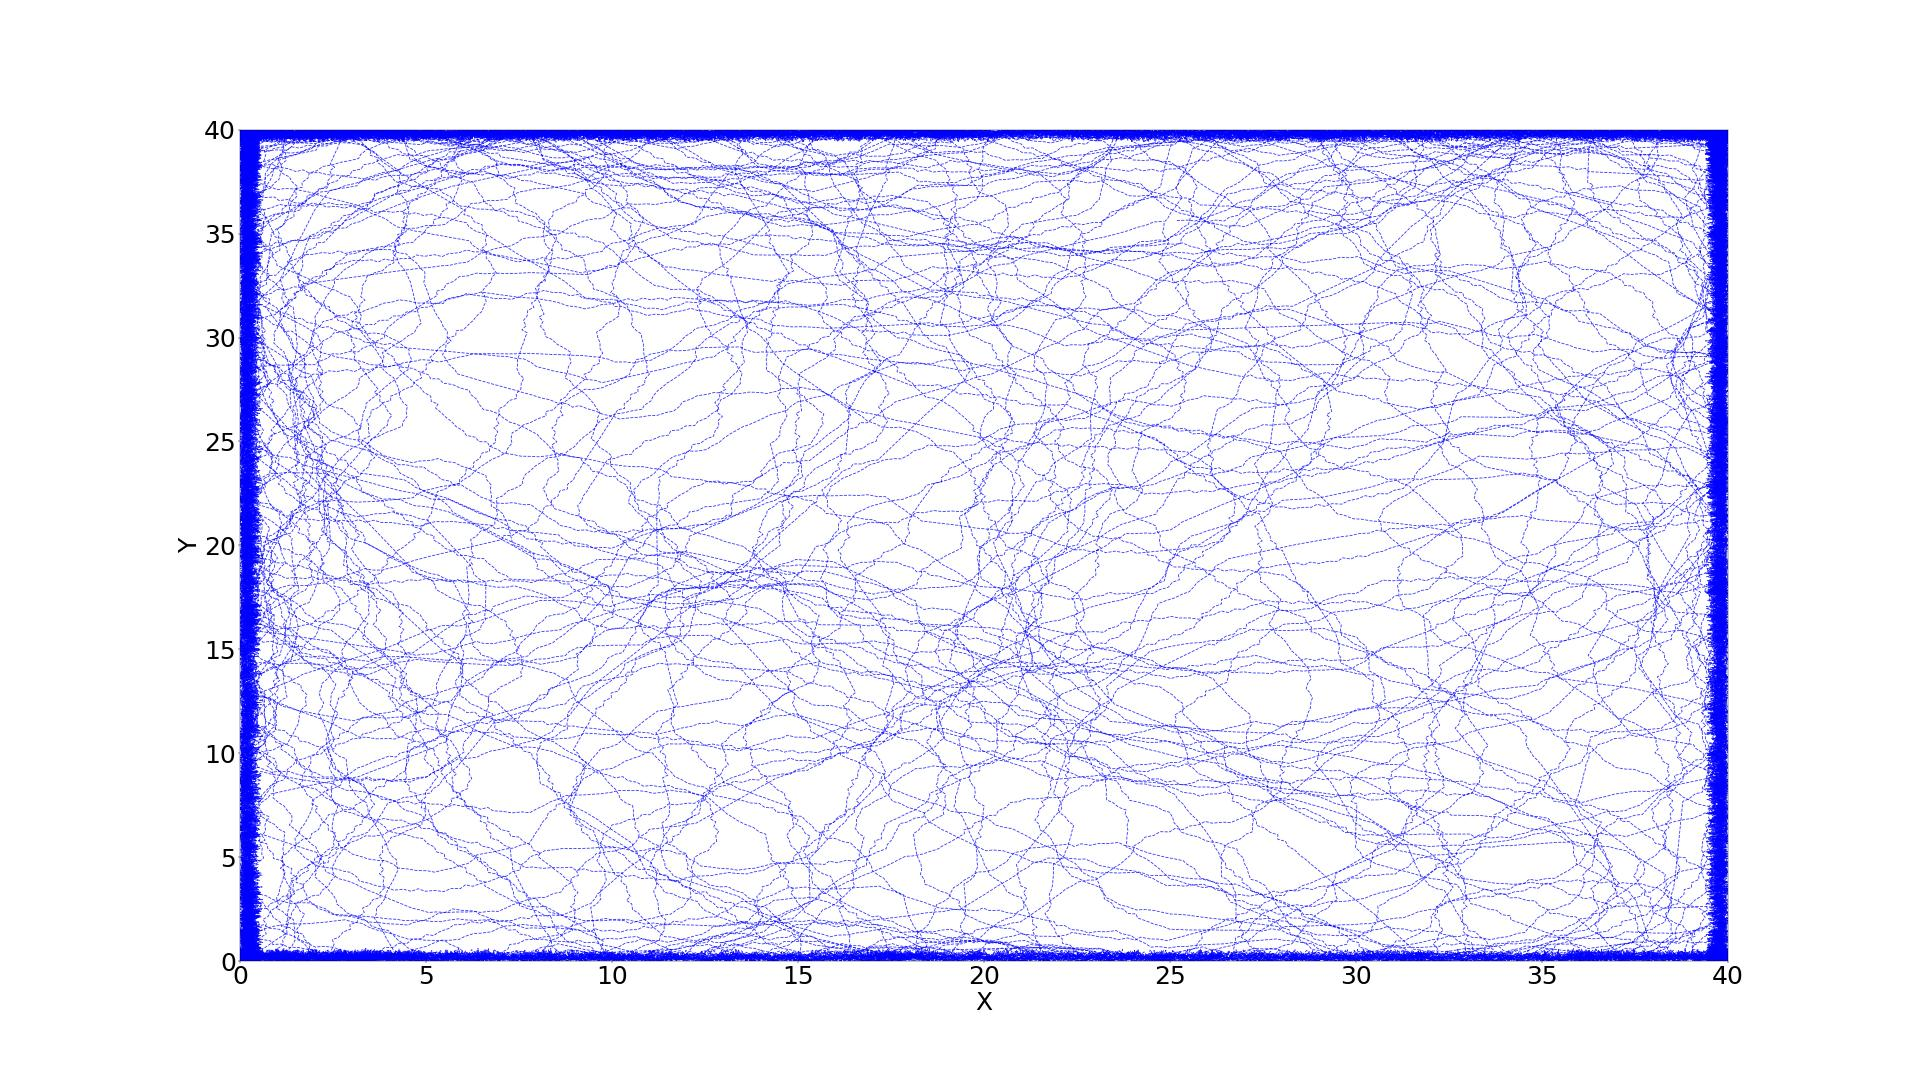
\includegraphics[width=1\linewidth]{LateX images/log/k/g2-1.4}
	\caption{Διάγραμμα διαδρομής ρομποτικού συστήματος για, $q = -1.4$ και $k = 0.751$.}
	\label{f:g82}	
\end{figure}

\begin{figure}[ht]
	\centering
	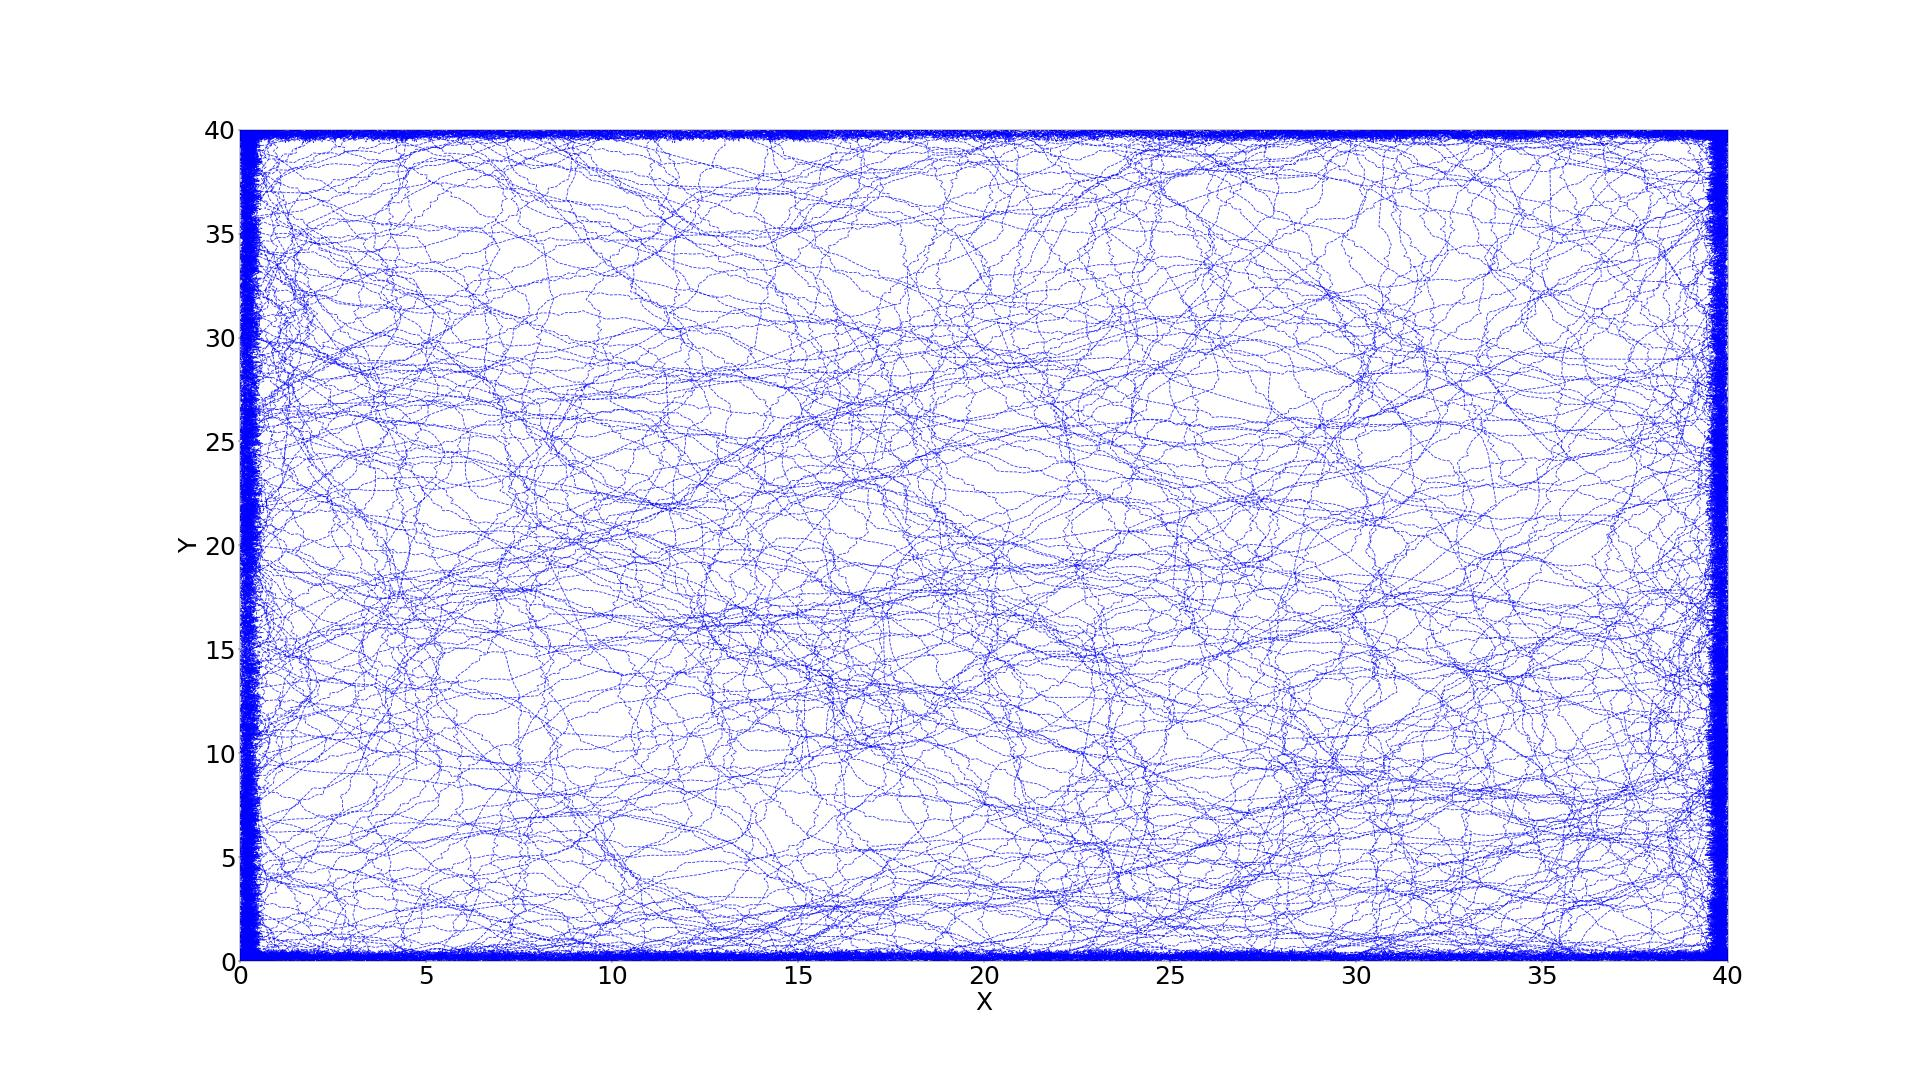
\includegraphics[width=1\linewidth]{LateX images/log/k/g3-1.4}
	\caption{Διάγραμμα διαδρομής ρομποτικού συστήματος για, $q = -1.4$ και $k = 0.76$.}
	\label{f:g83}	
\end{figure}

\clearpage

\section{Συμπεριφορά για Μεταβλητή Αρχική Θέση}
\label{sec:g2}
Για την απόκτηση μιας πλήρους εικόνας της συμπεριφοράς του ρομπότ απαιτείται η μελέτη της διαδρομής του υπό διαφορετικές αρχικές συντεταγμένες στο χώρο. Για αυτό τον λόγο επιλέχθηκαν  τρείς τυχαίες θέσεις \emph{(X,Y)} πέρα απο την θέση $[0,0]$ ενώ η παράμετρος διακλάδωσης \emph{k} παρέμεινε σταθερή $k = 0.68$.Για την συγκεκριμένη παράμετρο \emph{k} χρησιμοποιήθηκαν δύο διαφορετικές τιμές του \emph{q} \emph{(-2.1 , 1.9)} οι οποίες εμφανίζουν χαοτική συμπεριφορά.
Η προσομοίωση της κίνησης πραγματοποιήθηκε για $10^5$ βήματα, με αρχικές συνθήκες του χαοτικού συστήματος $x(0) = 0,  y(0) = 0.1$. και παράμετρο διακριτοποίησης $h = 0.2$. Έτσι, όπως και προηγουμένως για κάθε περίπτωση παράχθηκε το διάγραμμα της διαδρομής του ρομπότ και το ποσοστό καλυψιμότητάς της.

\subsection{Για \emph{q = -2.1}}

Αρχικά, ελέγχθηκε η περίπτωση το σύστημα να ξεκινάει από την αρχική θέση $(X,Y) = (0,0)$ και υπολογίστηκε ότι το ποσοστό κάλυψης είναι $54.121\%$. Στη συνέχεια, επιλέχθηκαν τυχαίες θέσεις στο χώρο και βρέθηκε ότι για $(X,Y) = (20,20)$ η καλυψιμότητα ήταν $56.35\%$ , ενώ για $(X,Y) = (5,20)$ η καλυψιμότητα ήταν $57.35\%$ και για $(X,Y) = (34,20)$ η καλυψιμότητα ήταν $53.52\%$. 

Συγκρίνοντας το Σχ. \ref{f:g84} με τα Σχ. \ref{f:g85}, \ref{f:g86}, \ref{f:g87} παρατηρούμε μικρή αύξηση σε σχέση με την αρχική περίπτωση για τις πρώτες δύο τυχαίες συντεταγμένες $(X,Y) = (20,20)$, $(X,Y) = (5,20)$ και μία μικρή μείωση για την τρίτη $(X,Y) = (34,20)$. Επομένως, η αρχική θέση του ρομπότ δεν επηρεάζει δραματικά την διαδρομή που θα ακολουθήσει το ρομποτικό όχημα.

Επιπλέον μπορούμε να δούμε πώς γεμίζει στην κάθε περίπτωση το ρομπότ την επιφάνεια στο Σχ. \ref{g93} όπου παρουσιάζονται σε κοινό διάγραμμα οι κινήσεις του συστήματος, για τις περιπτώσεις που παρουσιάστηκαν παραπάνω, δηλαδή για $q = -2.1$, $k = 0.68$, $(X,Y) = (0,0)$ \emph{(μαύρο χρώμα)}, $(X,Y) = (20,20)$ \emph{(κόκκινο χρώμα)}, $(X,Y) = (5,20)$ \emph{(μπλε χρώμα)}, $(X,Y) = (34,20)$ \emph{(κίτρινο χρώμα)}.


\begin{figure}[ht]
	\centering
	\begin{subfigure}[b]{0.55\textwidth}
		\centering
		\includegraphics[width=\textwidth]{LateX images/log/XY1/g2-2.1}
		\caption{Για $(X,Y) = (0,0)$.}
		\label{f:g84}
	\end{subfigure}
	\hfill
	\begin{subfigure}[b]{0.55\textwidth}
		\centering
		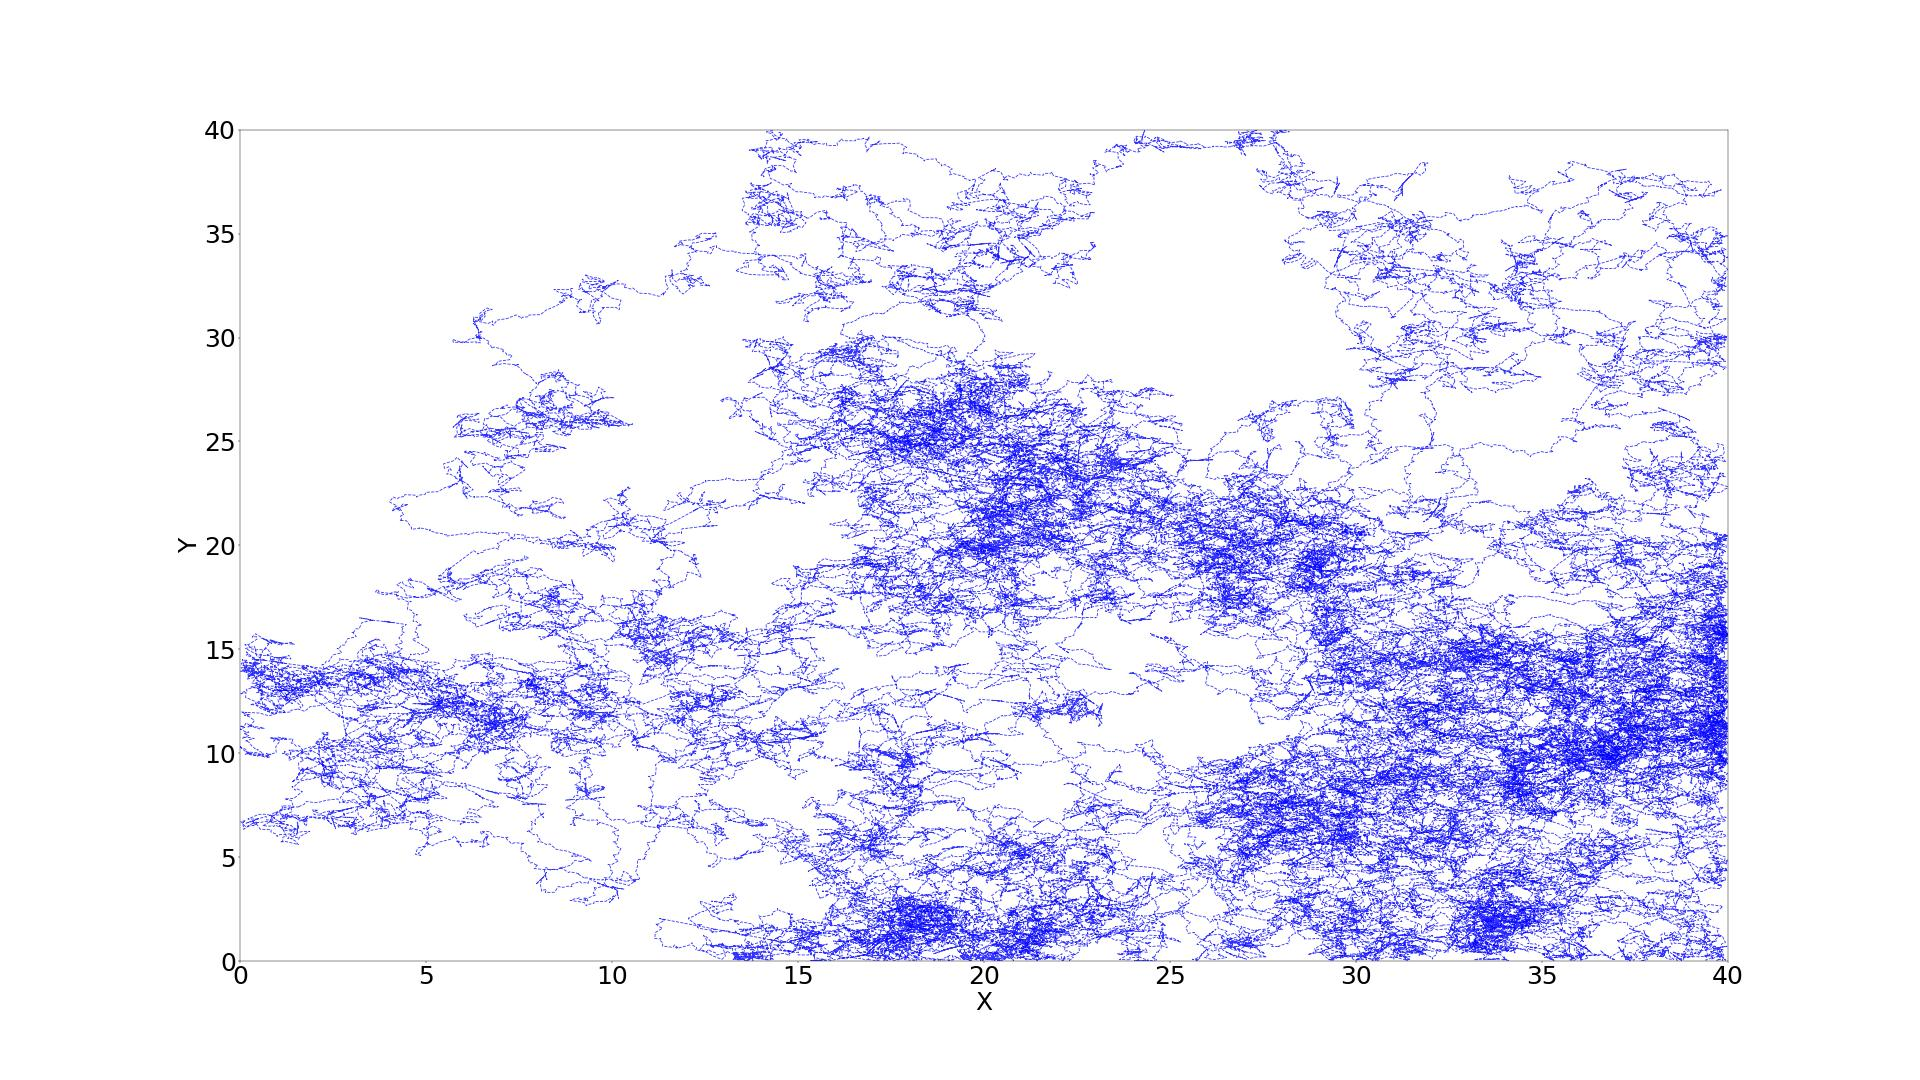
\includegraphics[width=\textwidth]{LateX images/log/XY1/g3-2.1}
		\caption{Για $(X,Y) = (20,20)$.}
		\label{f:g85}
	\end{subfigure}
	\hfill
	\begin{subfigure}[b]{0.55\textwidth}
		\centering
		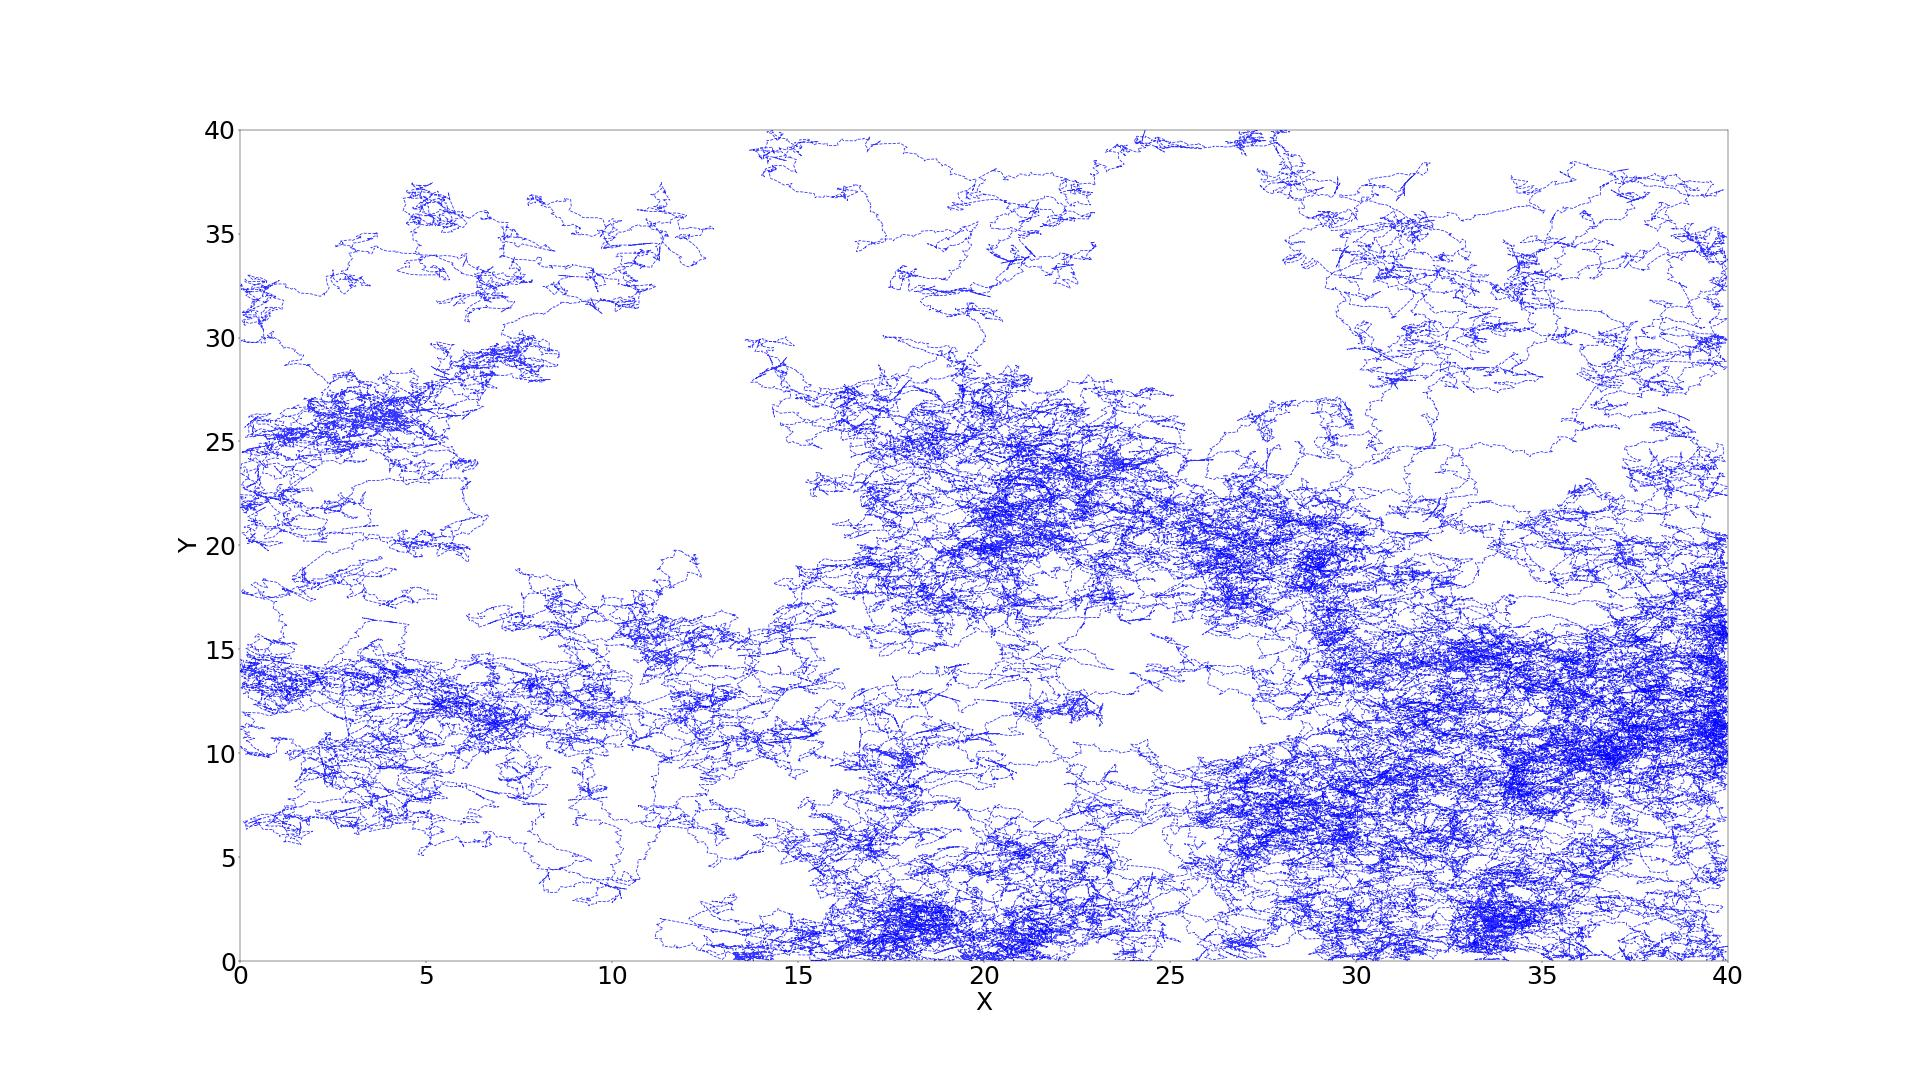
\includegraphics[width=\textwidth]{LateX images/log/XY1/g4-2.1}
		\caption{Για $(X,Y) = (5,20)$.}
		\label{f:g86}
	\end{subfigure}
	\hfill
	\begin{subfigure}[b]{0.55\textwidth}
		\centering
		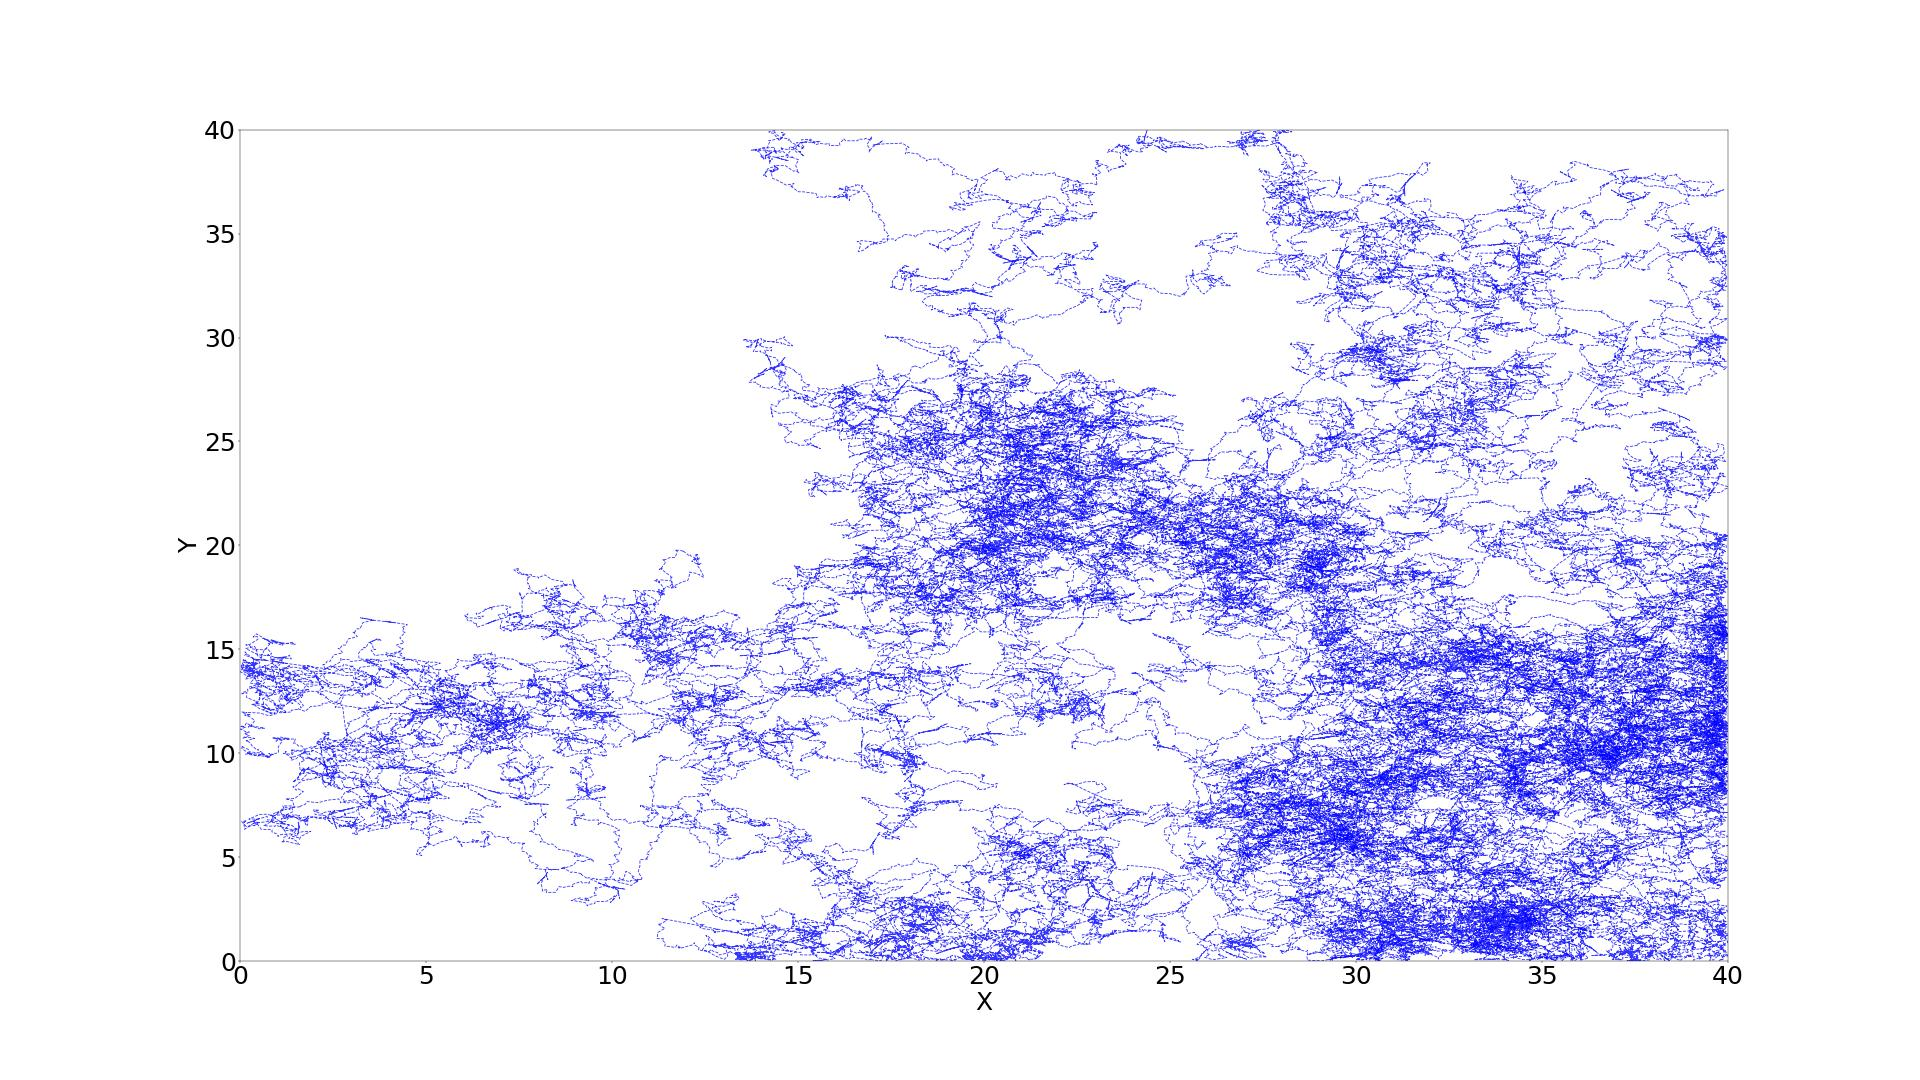
\includegraphics[width=\textwidth]{LateX images/log/XY1/g5-2.1}
		\caption{Για $(X,Y) = (34,20)$.}
		\label{f:g87}
	\end{subfigure}
	\hfill
\caption{Διαγράμματα διαδρομής ρομποτικού συστήματος για, $q = -1.9$, $k = 0.68$ και :}
\end{figure}

\begin{figure}[ht]
	\centering
	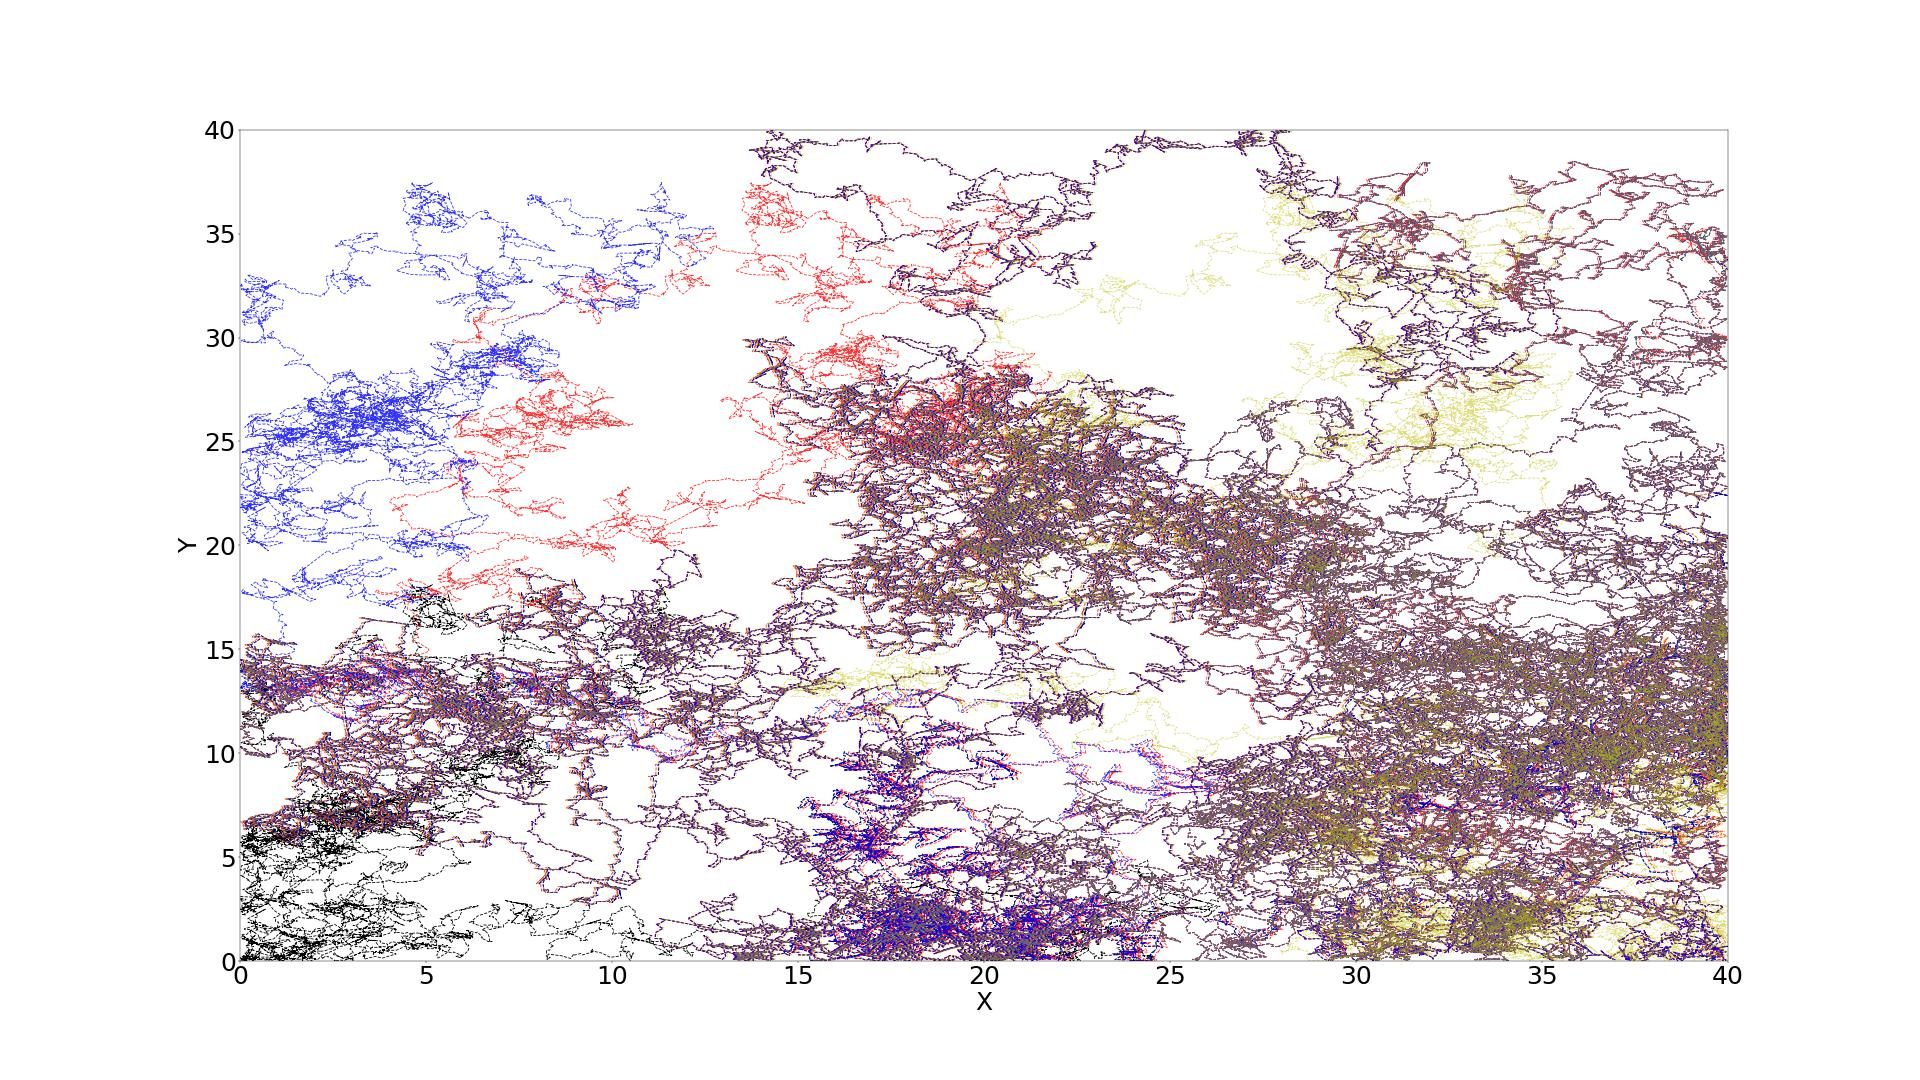
\includegraphics[width=1\linewidth]{LateX images/log/XY1/g2}
	\caption{Κοινό διάγραμμα διαδρομής ρομποτικού συστήματος για, $q = -2.1$, $k = 0.68$, $(X,Y) = (0,0)$ \emph{(μαύρο χρώμα)}, $(X,Y) = (20,20)$ \emph{(κόκκινο χρώμα)}, $(X,Y) = (5,20)$ \emph{(μπλε χρώμα)}, $(X,Y) = (34,20)$ \emph{(κίτρινο χρώμα)}.}
		\label{f:g93}	
	\end{figure}


\clearpage

\subsection{Για \emph{q = -1.9}}

Αρχικά, ελέγχθηκε η περίπτωση το σύστημα να ξεκινάει από την αρχική θέση $(X,Y) = (0,0)$ και υπολογίστηκε ότι το ποσοστό κάλυψης είναι $85.78\%$. Στη συνέχεια, επιλέχθηκαν τυχαίες θέσεις στο χώρο και βρέθηκε ότι για $(X,Y) = (5,15)$ η καλυψιμότητα ήταν $85.64\%$ , ενώ για $(X,Y) = (8,30)$ η καλυψιμότητα ήταν $85.1\%$ και για $(X,Y) = (36,26)$ η καλυψιμότητα ήταν $79.8\%$. 

Συγκρίνοντας το Σχ. \ref{f:g88} με τα Σχ. \ref{f:g89}, \ref{f:g90}, \ref{f:g91} παρατηρούμε μικρή μείωση σε σχέση με την αρχική περίπτωση για τις πρώτες δύο τυχαίες συντεταγμένες $(X,Y) = (5,15)$, $(X,Y) = (8,30)$ και μία σχετικά μεγαλύτερη μείωση (γύρω στο $6\%$) για την τρίτη $(X,Y) = (36,6)$. Επομένως, η αρχική θέση του ρομπότ δεν επηρεάζει δραματικά την διαδρομή που θα ακολουθήσει το ρομποτικό όχημα, ακόμα και στην τρίτη περίπτωση που η διαφορά είναι  $6\%$

Επίσης μπορούμε να δούμε πώς γεμίζει στην κάθε περίπτωση το ρομπότ την επιφάνεια στο Σχ. \ref{f:g92} όπου
παρουσιάζονται σε κοινό διάγραμμα οι κινήσεις του συστήματος, για τις περιπτώσεις που παρουσιάστηκαν παραπάνω, δηλαδή για $(X,Y) = (0,0)$ \emph{(μαύρο χρώμα)}, $(X,Y) = (5,15)$ \emph{(κόκκινο χρώμα)}, $(X,Y) = (8,30)$ \emph{(μπλε χρώμα)}, $(X,Y) = (36,6)$ \emph{(κίτρινο χρώμα)}.

\begin{figure}[ht]
	\centering
	\begin{subfigure}[b]{0.55\textwidth}
		\centering
		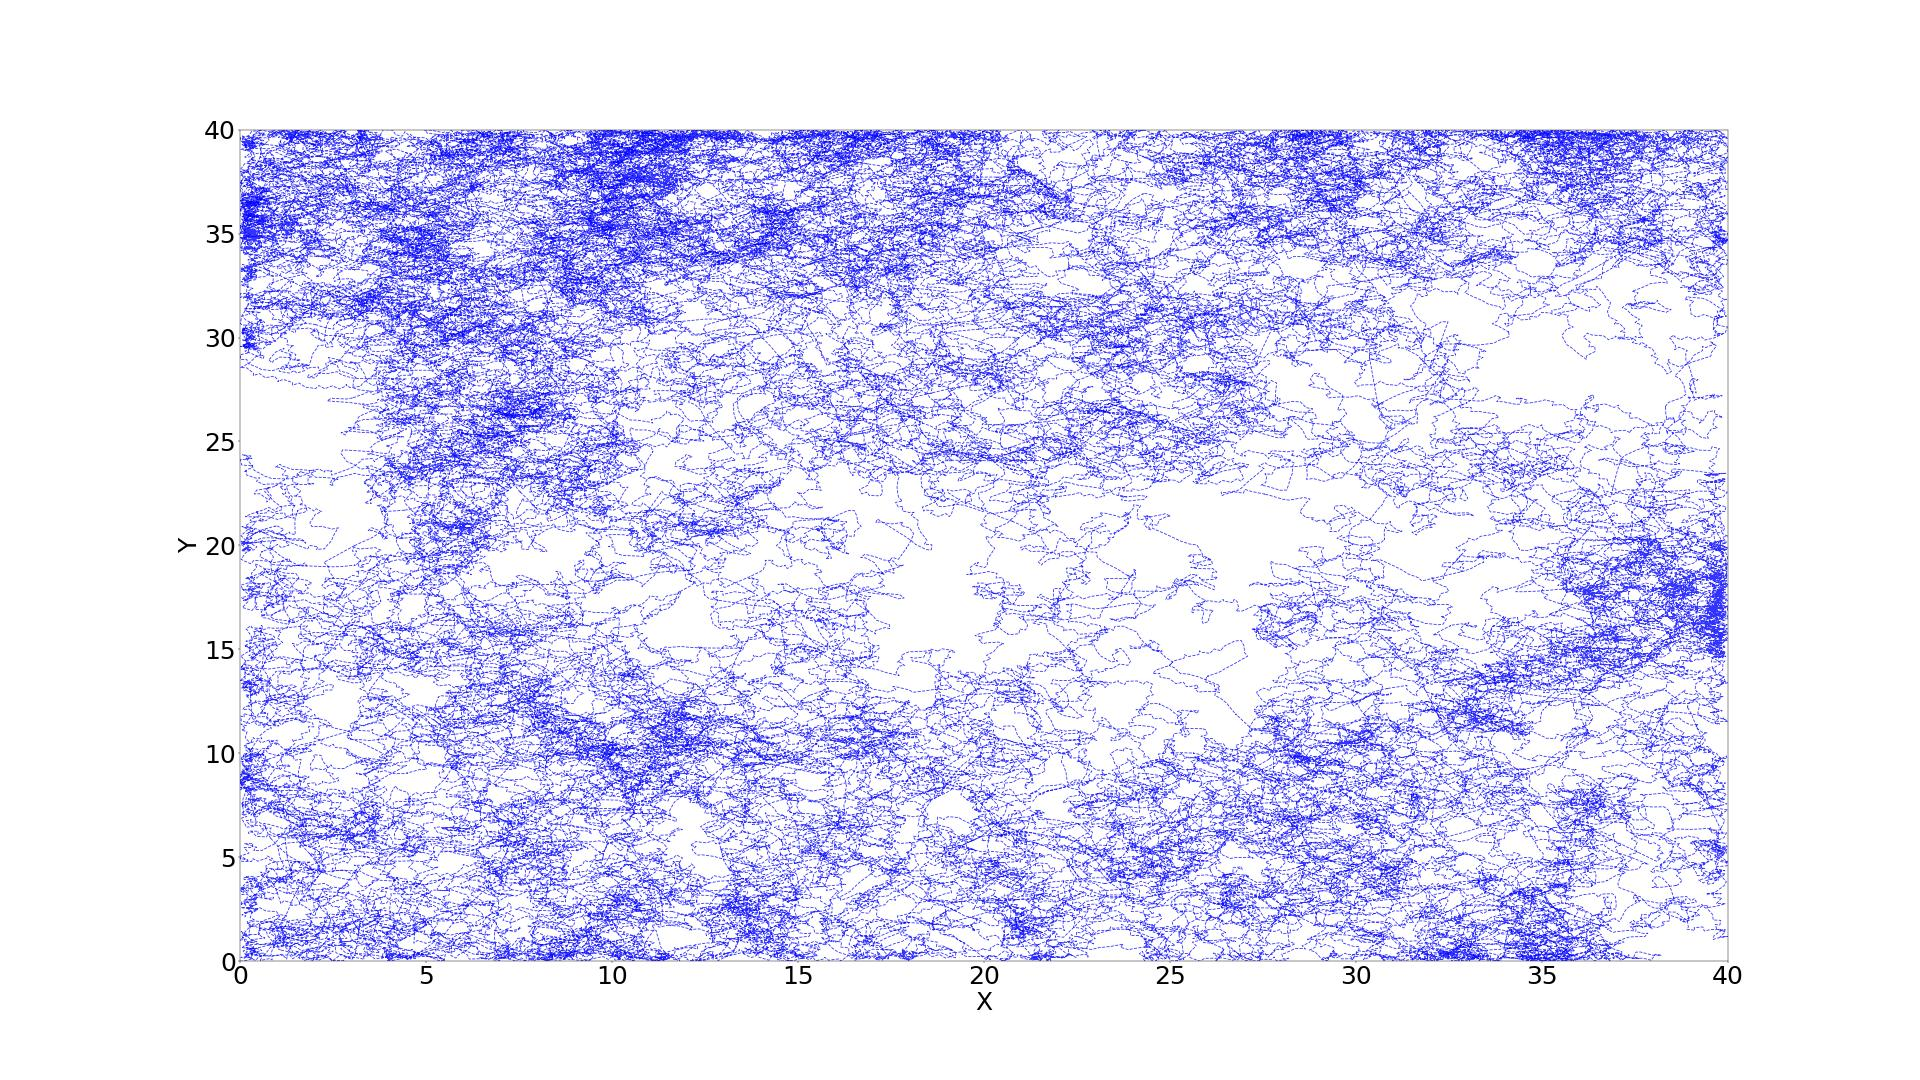
\includegraphics[width=\textwidth]{LateX images/log/XY1/g1-1.9}
		\caption{Για $(X,Y) = (0,0)$.}
		\label{f:g88}
	\end{subfigure}
	\hfill
	\begin{subfigure}[b]{0.55\textwidth}
		\centering
		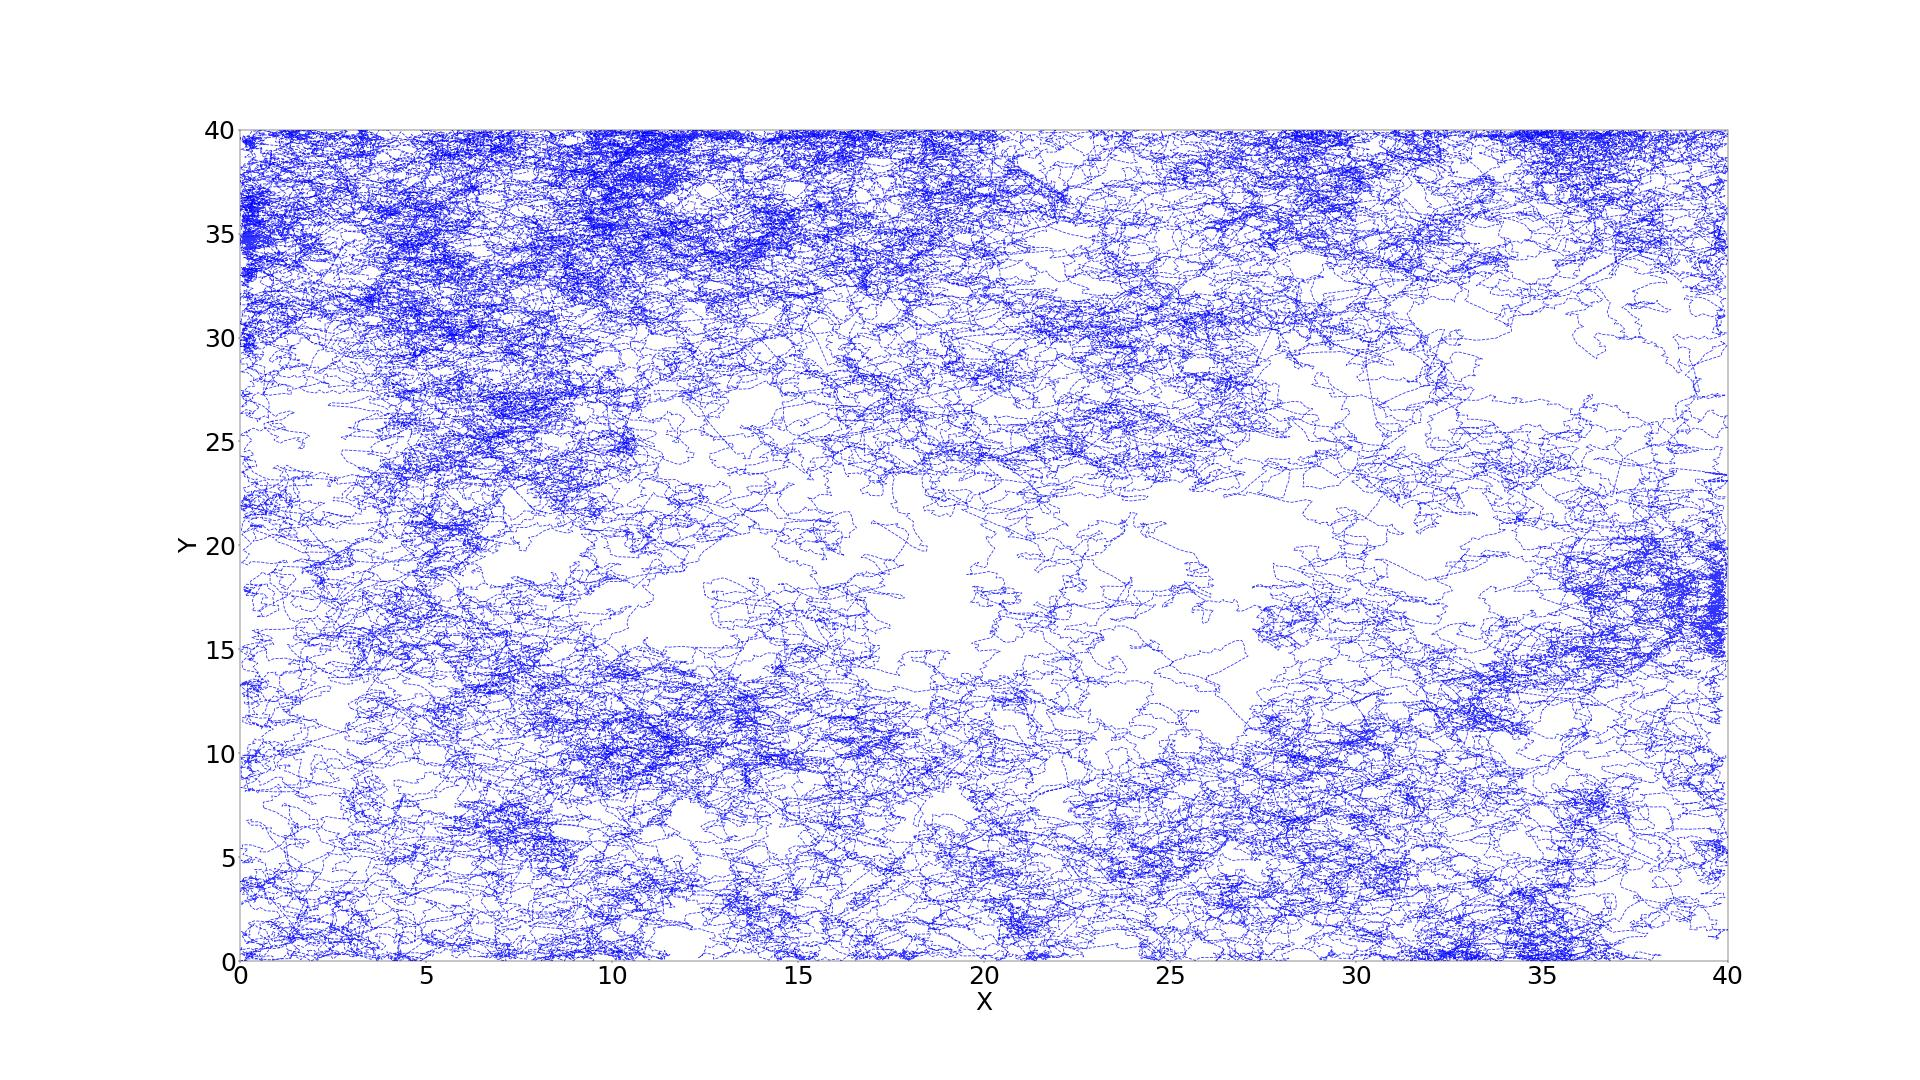
\includegraphics[width=\textwidth]{LateX images/log/XY1/g2-1.9}
		\caption{Για $(X,Y) = (5,15)$.}
		\label{f:g89}
	\end{subfigure}
	\hfill
	\begin{subfigure}[b]{0.55\textwidth}
		\centering
		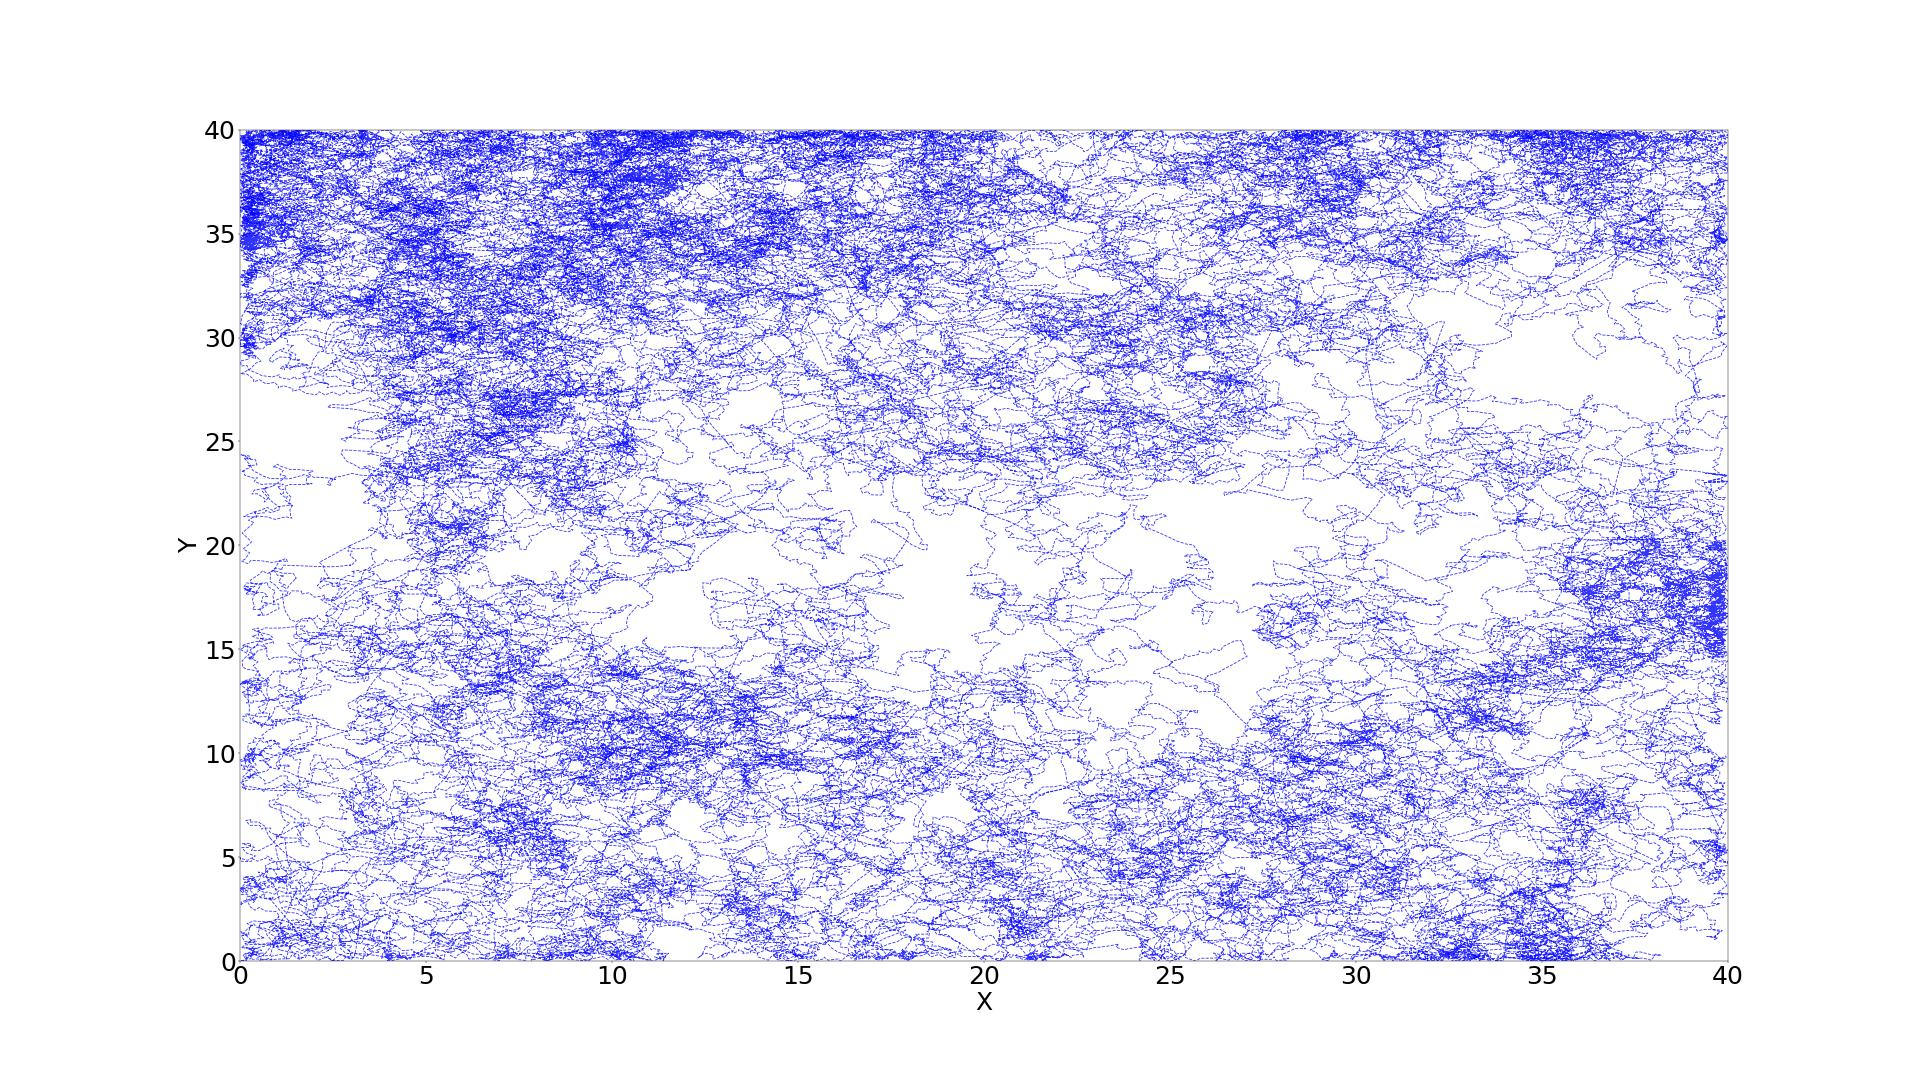
\includegraphics[width=\textwidth]{LateX images/log/XY1/g3-1.9}
		\caption{Για $(X,Y) = (8,30)$.}
		\label{f:g90}
	\end{subfigure}
	\hfill
	\begin{subfigure}[b]{0.55\textwidth}
		\centering
		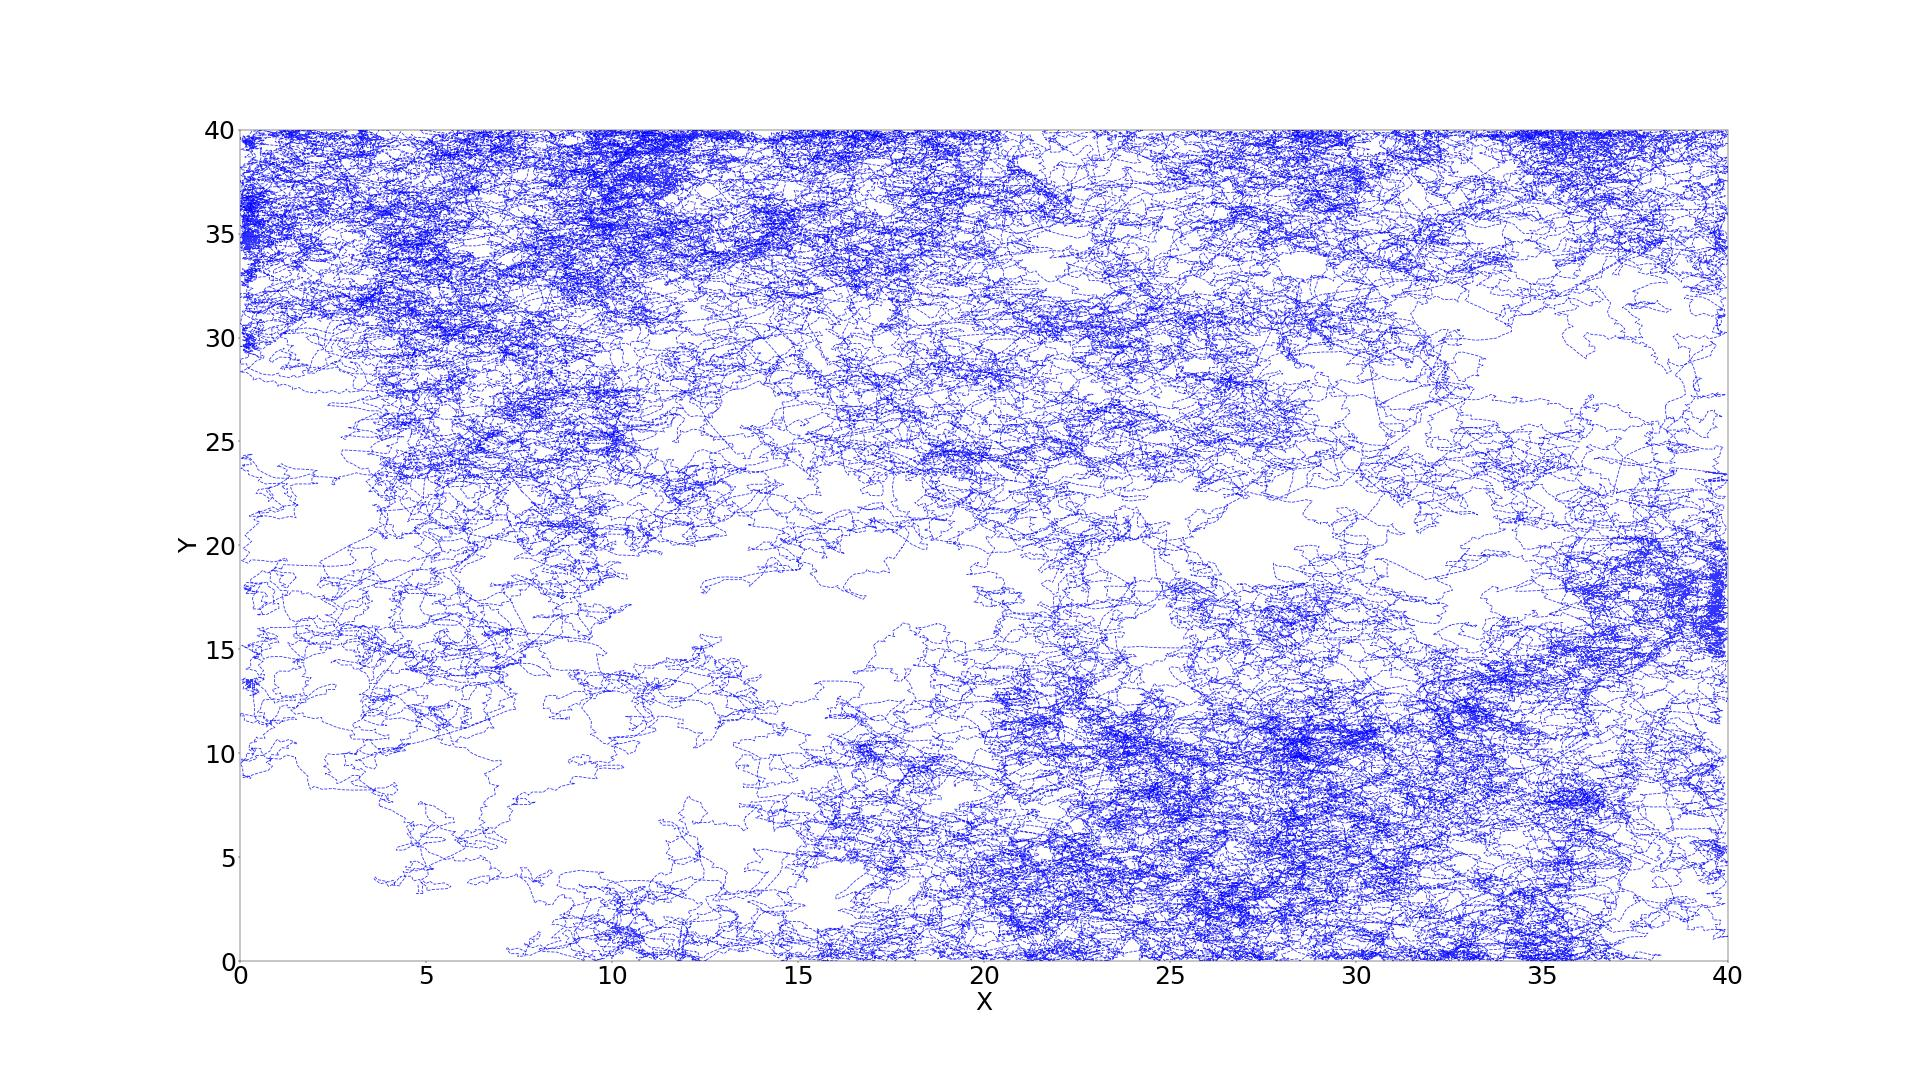
\includegraphics[width=\textwidth]{LateX images/log/XY1/g4-1.9}
		\caption{Για $(X,Y) = (36,6)$.}
		\label{f:g91}
	\end{subfigure}
	\hfill
	\caption{Διαγράμματα διαδρομής ρομποτικού συστήματος για, $q = -1.9$, $k = 0.68$ και :}
\end{figure}


\begin{figure}[ht]
	\centering
	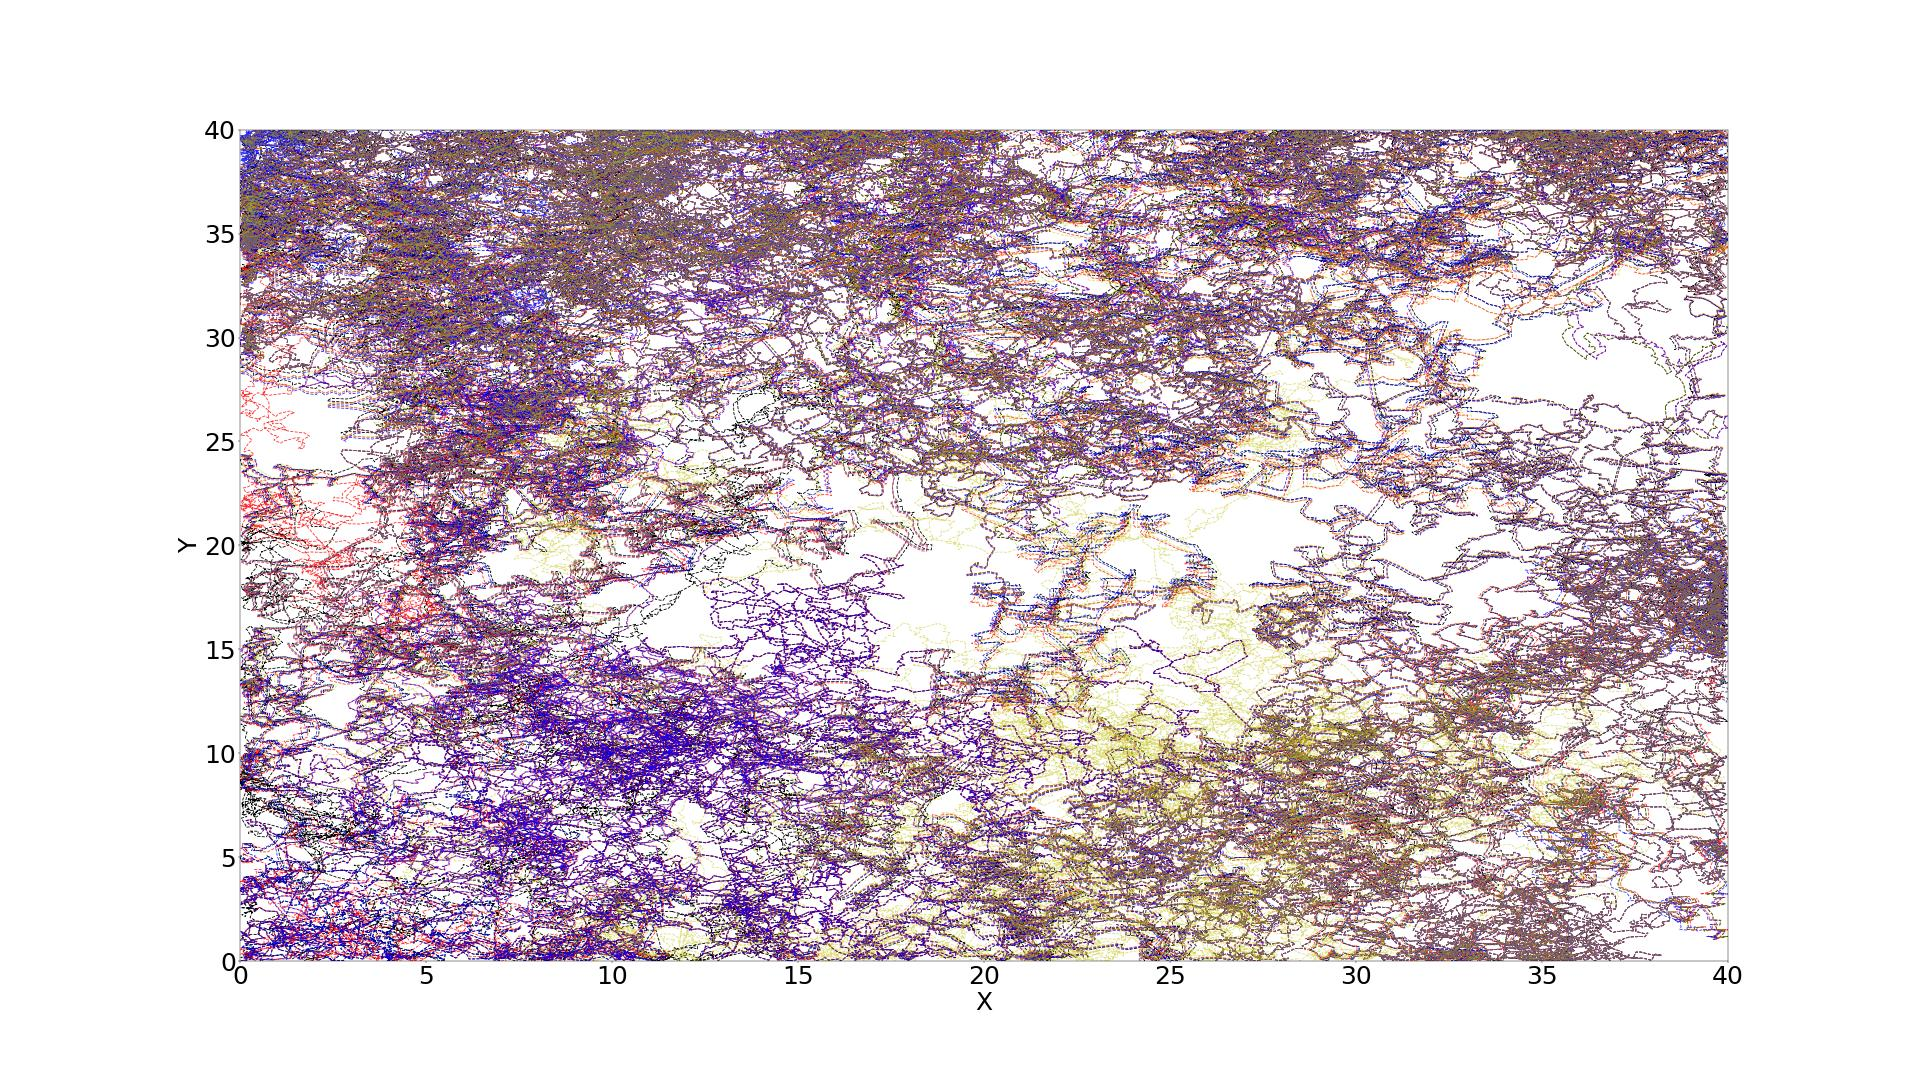
\includegraphics[width=1\linewidth]{LateX images/log/XY1/g1}
	\caption{Κοινό διάγραμμα διαδρομής ρομποτικού συστήματος για, $q = -1.9$, $k = 0.68$, $(X,Y) = (0,0)$ \emph{(μαύρο χρώμα)}, $(X,Y) = (5,15)$ \emph{(κόκκινο χρώμα)}, $(X,Y) = (8,30)$ \emph{(μπλε χρώμα)}, $(X,Y) = (36,6)$ \emph{(κίτρινο χρώμα)}.}
	\label{f:g92}	
\end{figure}


\clearpage


\section{Συμπεριφορά για Μεταβαλητές Αρχικές Συνθήκες}
\label{sec:g3}
Συνεχίζοντας την μελέτη αξίζει να ερευνηθεί πως συμπεριφέρεται το ρομποτικό σύστημα όταν μεταβληθούν οι αρχικές συνθήκες του χαοτικού δυναμικού συστήματος $x(0)$, $y(0)$. 

Στην συγκεριμένη μελέτη που πραγματοποιήθηκε λάβαμε υπόψη δύο περιπτώσεις χαοτικών συστημάτων.
Στην πρώτη περίπτωση επιλέχθηκε η παράμετρος \emph{q} να ισούται $q = -1.4$ και η παράμετρος διακλάδωσης \emph{k} να ισούται $k = 0.75$. Στην δεύτερη περίπτωση  η \emph{q} ισούται $q = -1.6$ και η παράμετρος διακλάδωσης  \emph{k} να ισούται $k = 0.9$. 

Επιπλέον, το ρομπότ εκτέλεσε $10^5$ βήματα.Η αρχική θέση του ρομποτικού συστήματος που επιλέχθηκε και για τις δύο περιπτώσεις είναι  $(X,Y) = (0,0)$, όπως και η παράμετρος διακριτοποίησης που είναι $h = 0.2$. Έτσι, για κάθε περίπτωση παράχθηκε το διάγραμμα της διαδρομής του ρομπότ και υπολογίστηκε το ποσοστό κάλυψης.

\subsection{Για \emph{q = -1.4}}

Στα Σχ.\ref{f:g94}, \ref{f:g95}, \ref{f:g96}, \ref{f:g97} παρατίθενται τα διαγράμματα κίνησης του συστήματος για $q =-1.4$ , $k = 0.75$ και $(x,y) = (-0.1,0.1)$ όπου η καλυψιμότητα είναι $10.35\%$ , $(x,y) = (0.1,0.5)$ όπου η καλυψιμότητα είναι $15.23\%$, $(x,y) = (-0.1,1)$ όπου η καλυψιμότητα είναι $13.3\%$, $(x,y) = (0.5,1)$ όπου η καλυψιμότητα είναι $86.5\%$ αντίστοιχα.

Επίσης στο Σχ. \ref{f:g98} παρατίθεται το κοινό διάγραμμα των διαφορετικών αρχικών συνθηκών με την καθεμία να συμβολίζεται με διαφορετικό χρώμα, δηλαδή για $(x,y) = (-0.1,0.1)$ \emph{(μαύρο χρώμα)}, $(x,y) = (0.1,0.5)$ \emph{(κόκκινο χρώμα)}, $(x,y) = (0.1,0.5)$ \emph{(μπλε χρώμα)}, $(x,y) = (0.5,1)$ \emph{(ροζ(magenta) χρώμα)}

\begin{figure}[ht]
	\centering
	\begin{subfigure}[b]{0.55\textwidth}
		\centering
		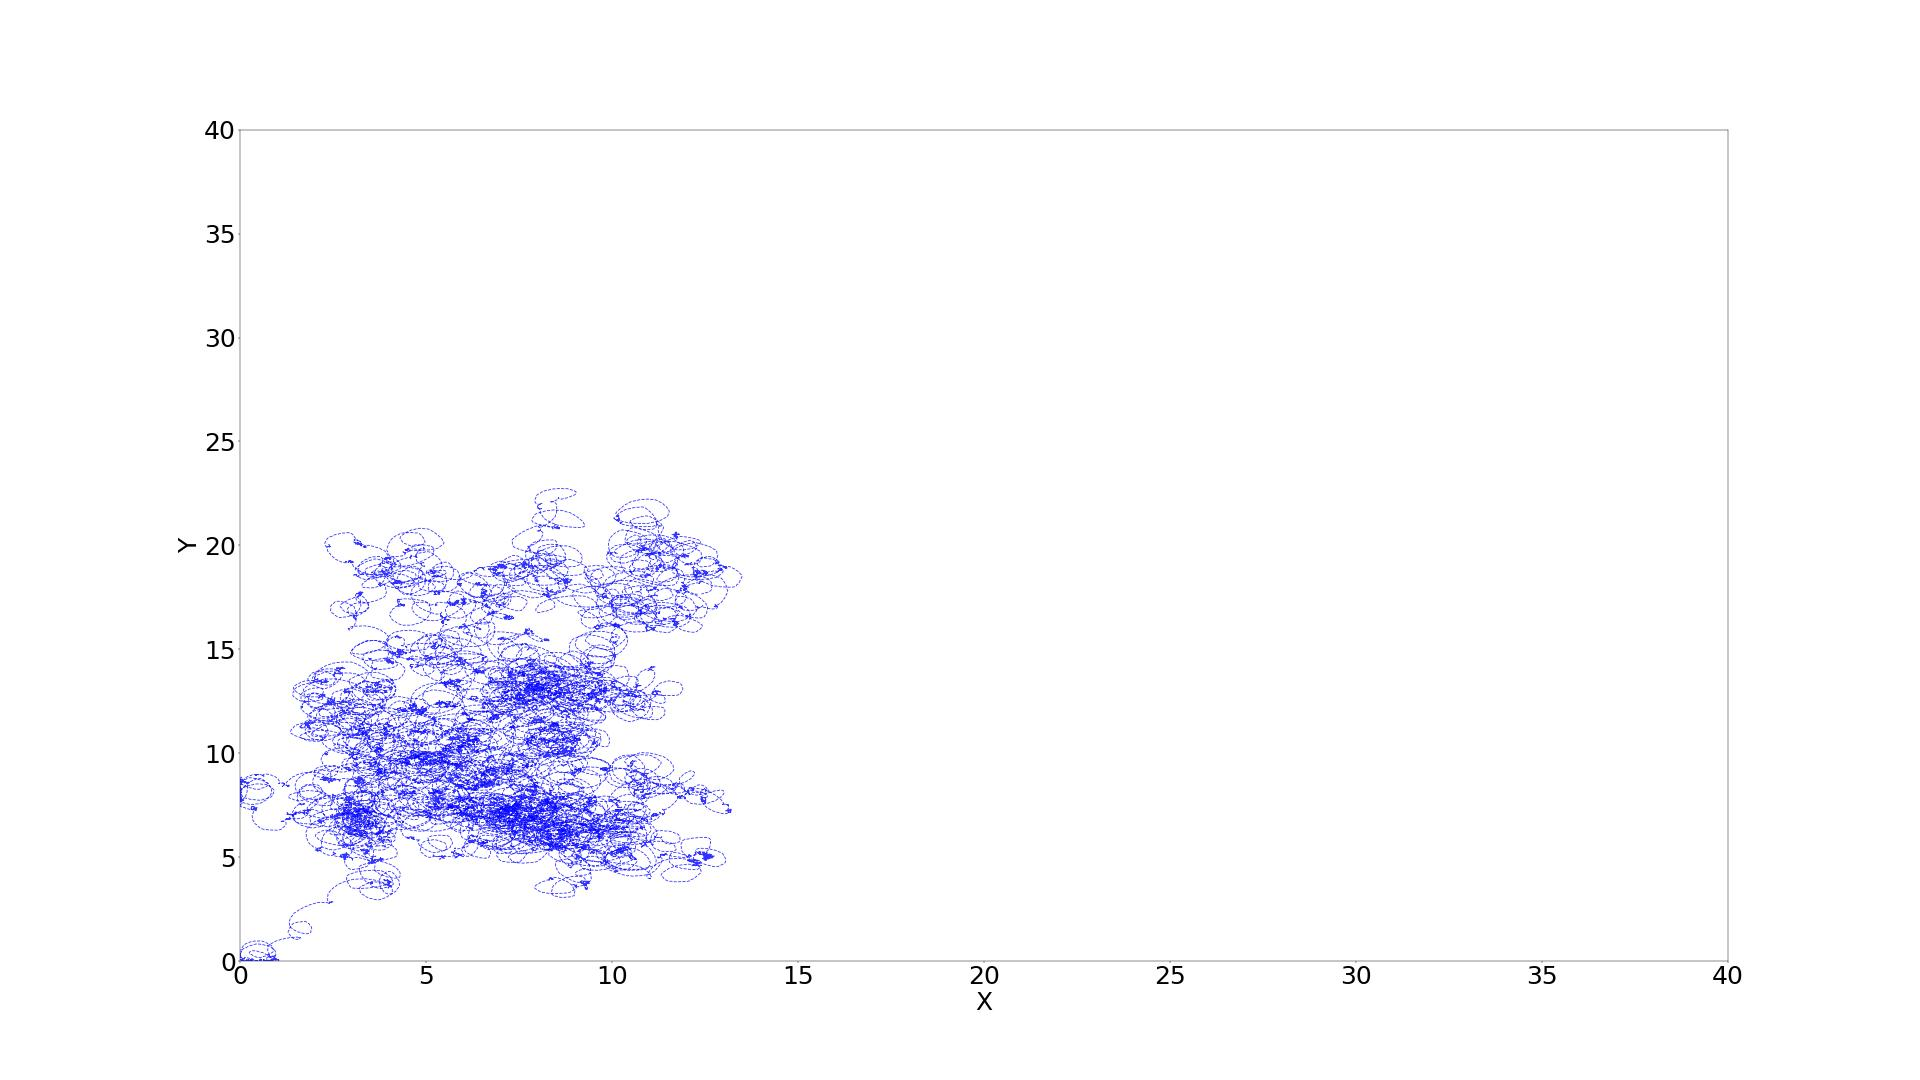
\includegraphics[width=\textwidth]{LateX images/log/xy/g1-1.4}
		\caption{Για $(x,y) = (-0.1,0.1)$.}
		\label{f:g94}
	\end{subfigure}
	\hfill
	\begin{subfigure}[b]{0.55\textwidth}
		\centering
		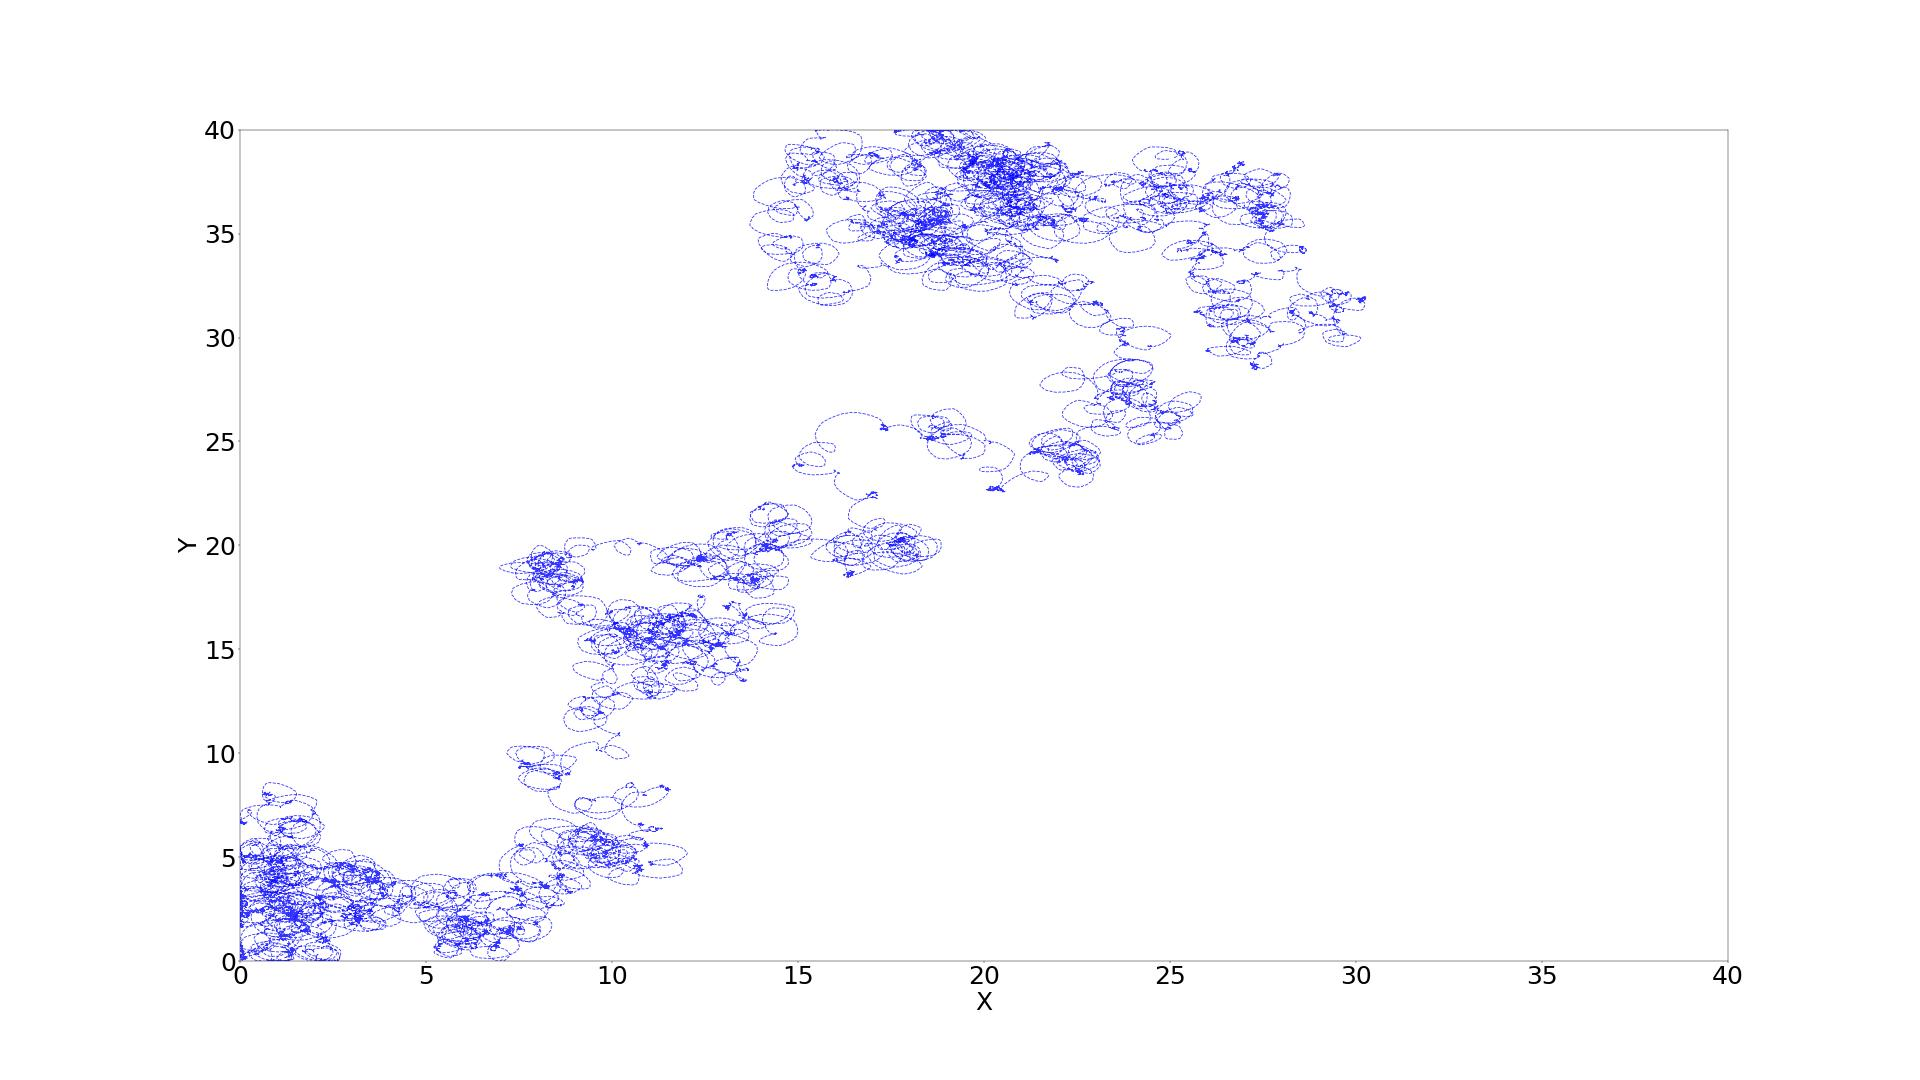
\includegraphics[width=\textwidth]{LateX images/log/xy/g2-1.4}
		\caption{Για $(x,y) = (0.1,0.5)$.}
		\label{f:g95}
	\end{subfigure}
	\hfill
	\begin{subfigure}[b]{0.55\textwidth}
		\centering
		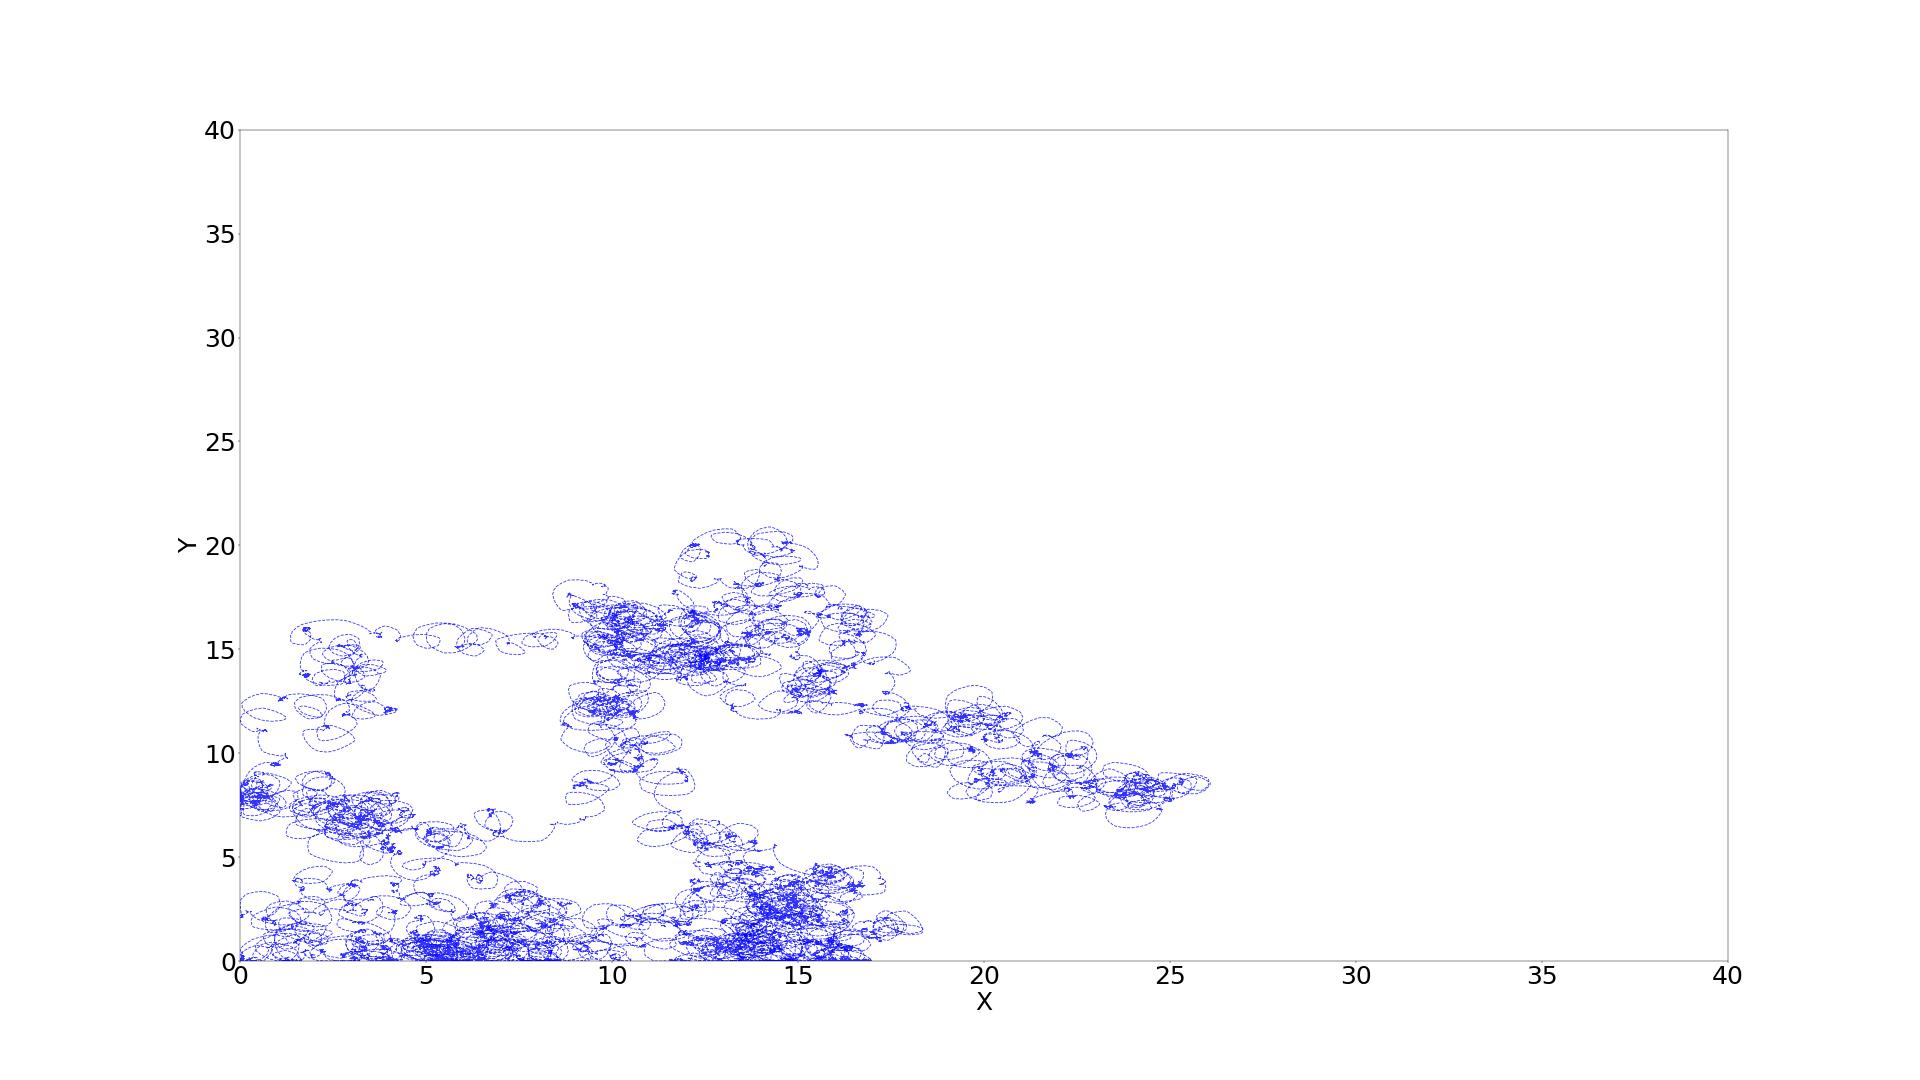
\includegraphics[width=\textwidth]{LateX images/log/xy/g3-1.4}
		\caption{Για $(x,y) = (-0.1,1)$.}
		\label{f:g96}
	\end{subfigure}
	\hfill
	\begin{subfigure}[b]{0.55\textwidth}
		\centering
		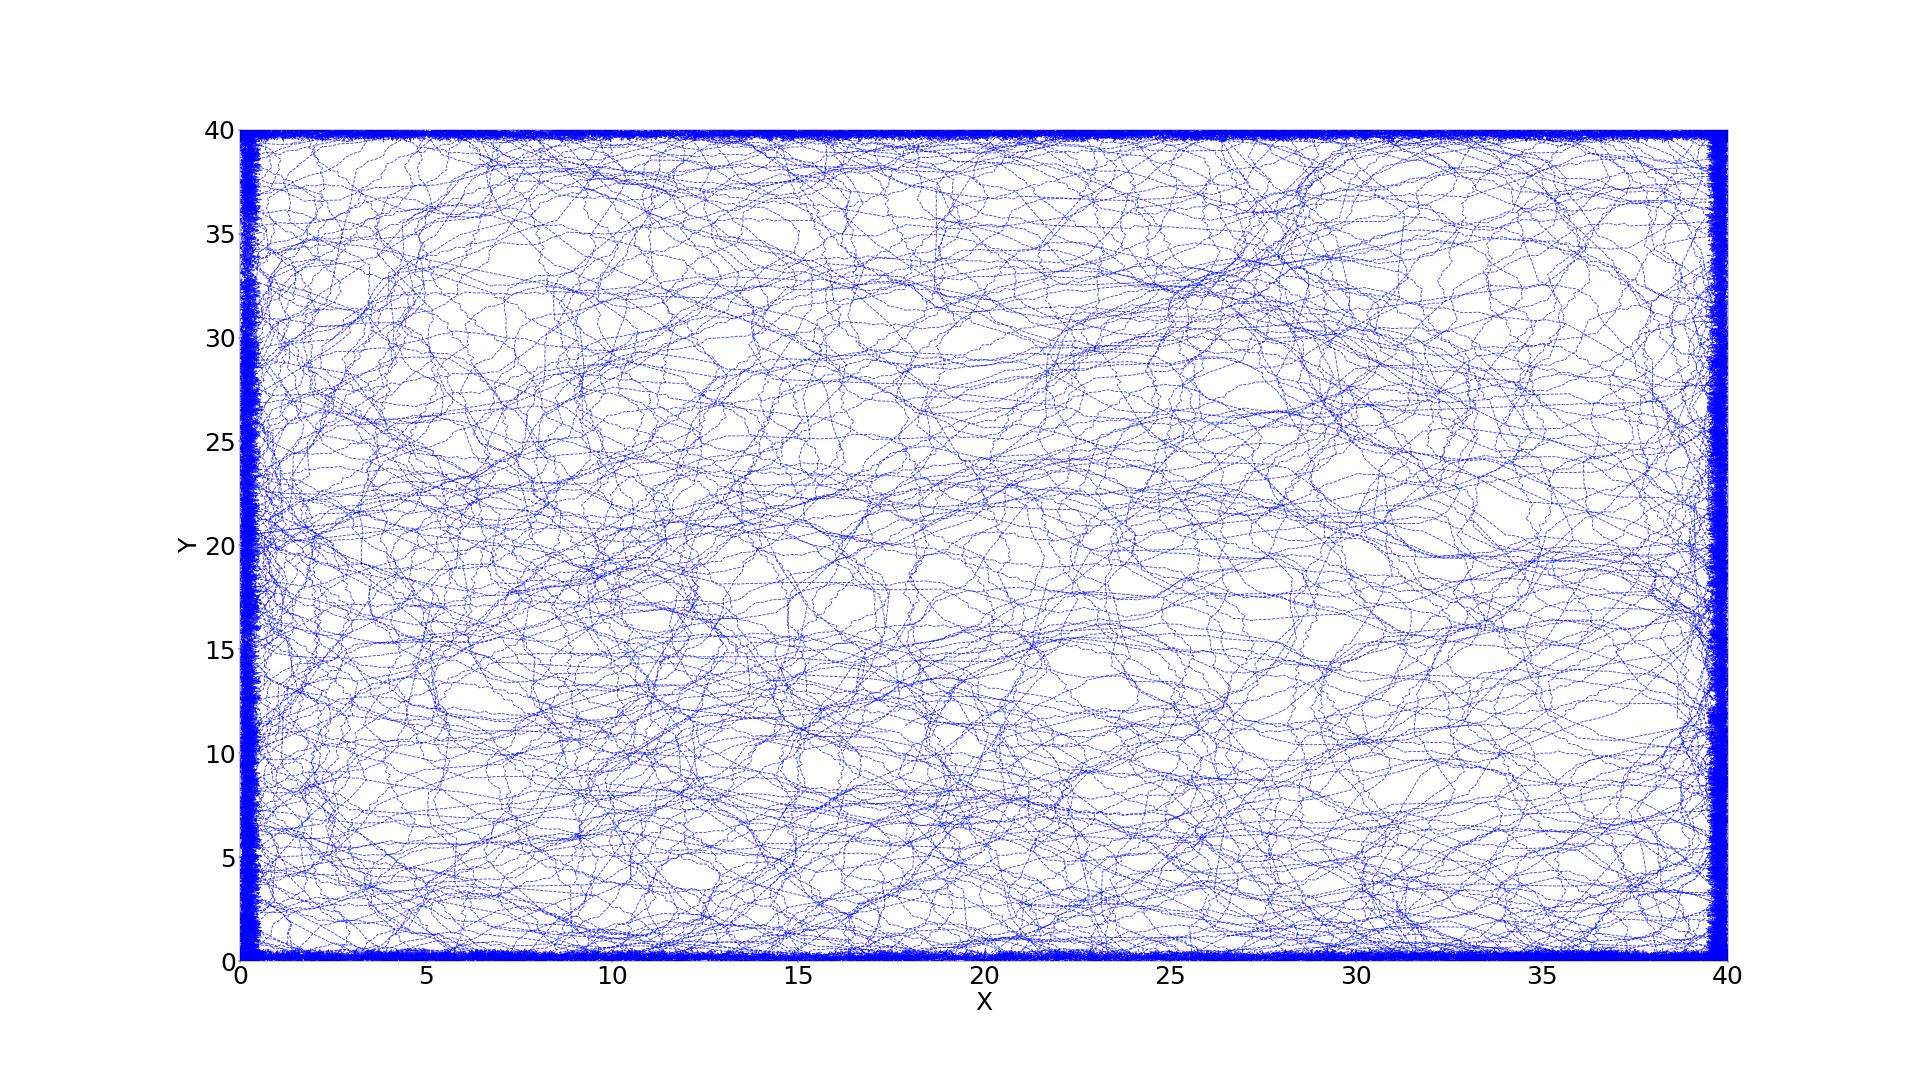
\includegraphics[width=\textwidth]{LateX images/log/xy/g4-1.4}
		\caption{Για $(x,y) = (0.5,1)$.}
		\label{f:g97}
	\end{subfigure}
	\hfill
	\caption{Διαγράμματα διαδρομής ρομποτικού συστήματος για, $q = -1.4$, $k = 0.75$ και :}
\end{figure}

\begin{figure}[ht]
	\centering
	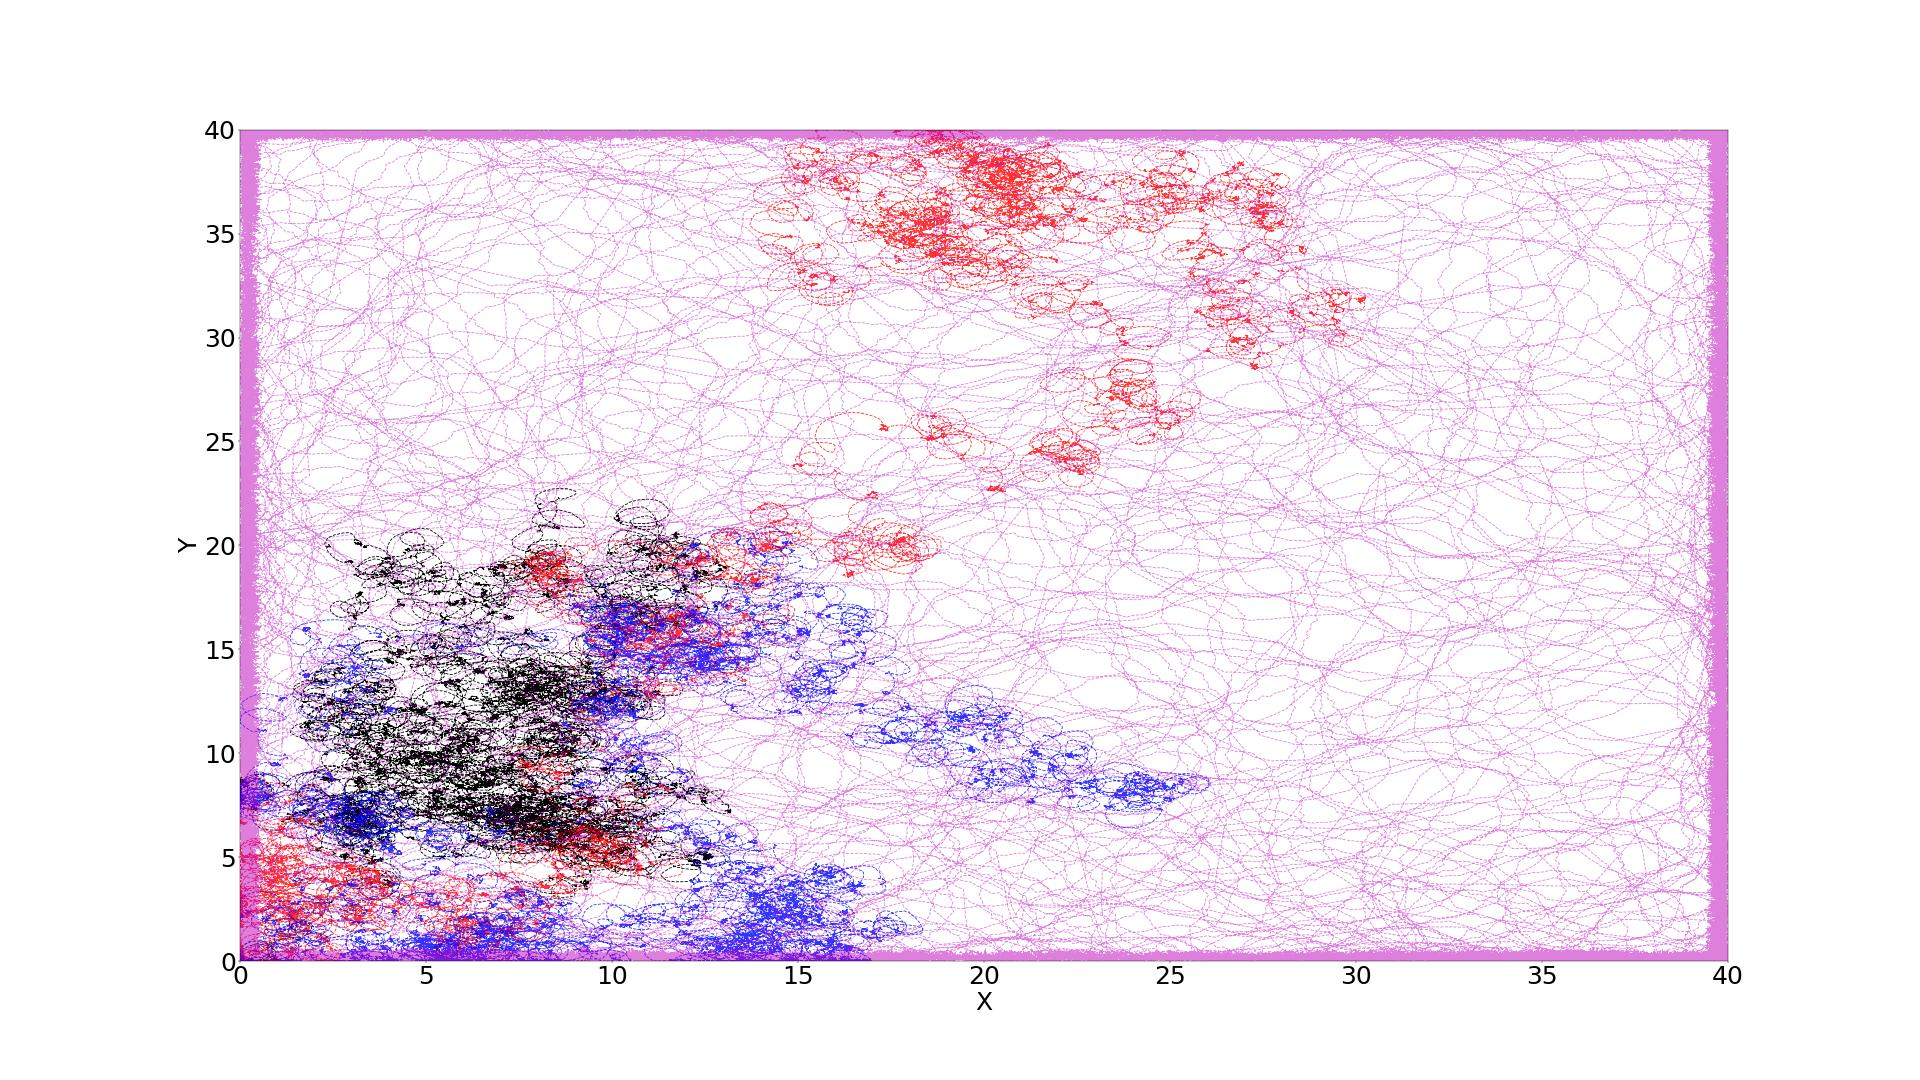
\includegraphics[width=1\linewidth]{LateX images/log/xy/g2}
	\caption{Κοινό διάγραμμα διαδρομής ρομποτικού συστήματος για, $q = -1.4$, $k = 0.75$, $(x,y) = (-0.1,0.1)$ \emph{(μαύρο χρώμα)}, $(x,y) = (0.1,0.5)$ \emph{(κόκκινο χρώμα)}, $(x,y) = (0.1,0.5)$ \emph{(μπλε χρώμα)}, $(x,y) = (0.5,1)$ \emph{(ροζ(magenta) χρώμα)}.}
	\label{f:g98}	
\end{figure}

\clearpage

\subsection{Για \emph{q = -1.6}}

Στην συγκεκριμένη περίπτωση επειδή τα ποσοστά κάλυψης για κάθε αρχική συνθήκη που επιλέχθηκε ήταν πολύ κοντά μεταξύ τους, δηλαδή  για $q =-1.6$ , $k = 0.9$ και $(x,y) = (0.1,0.5)$ το ποσοστό είναι $96.1\%$ , $(x,y) = (-0.1,0.5)$ το ποσοστό είναι $95.6\%$, $(x,y) = (-0.1,2)$ το ποσοστό είναι $94.4\%$, $(x,y) = (0.5,1.5)$ το ποσοστό είναι $94.2\%$ και $(x,y) = (0.8,1.2)$ το ποσοστό είναι $95.9\%$, δεν παράχθηκαν ξεχωριστά διαγράμματα διαδρομής του ρομποτικόυ συστήματος , εφόσον η πιο ακραία διαφορά είναι $2\%$.
Αντιθέτως παράχθηκε ένα κοινό διάγραμμα το οποίο φαίνεται στο Σχ. \ref{f:g99}. Το κάθε ζεύγος αρχικών συνθηκών συμβολίζεται με διαφορετικό χρώμα. Για $(x,y) = (0.1,0.5)$ \emph{(μαύρο χρώμα)} , $(x,y) = (-0.1,0.5)$ \emph{(κόκκινο χρώμα)} , $(x,y) = (-0.1,2)$ \emph{(μπλέ χρώμα)}, $(x,y) = (0.5,1.5)$ \emph{(ροζ(magenta) χρώμα)} και $(x,y) = (0.8,1.2)$ \emph{(κίτρινο χρώμα)}.

\begin{figure}[ht]
	\centering
	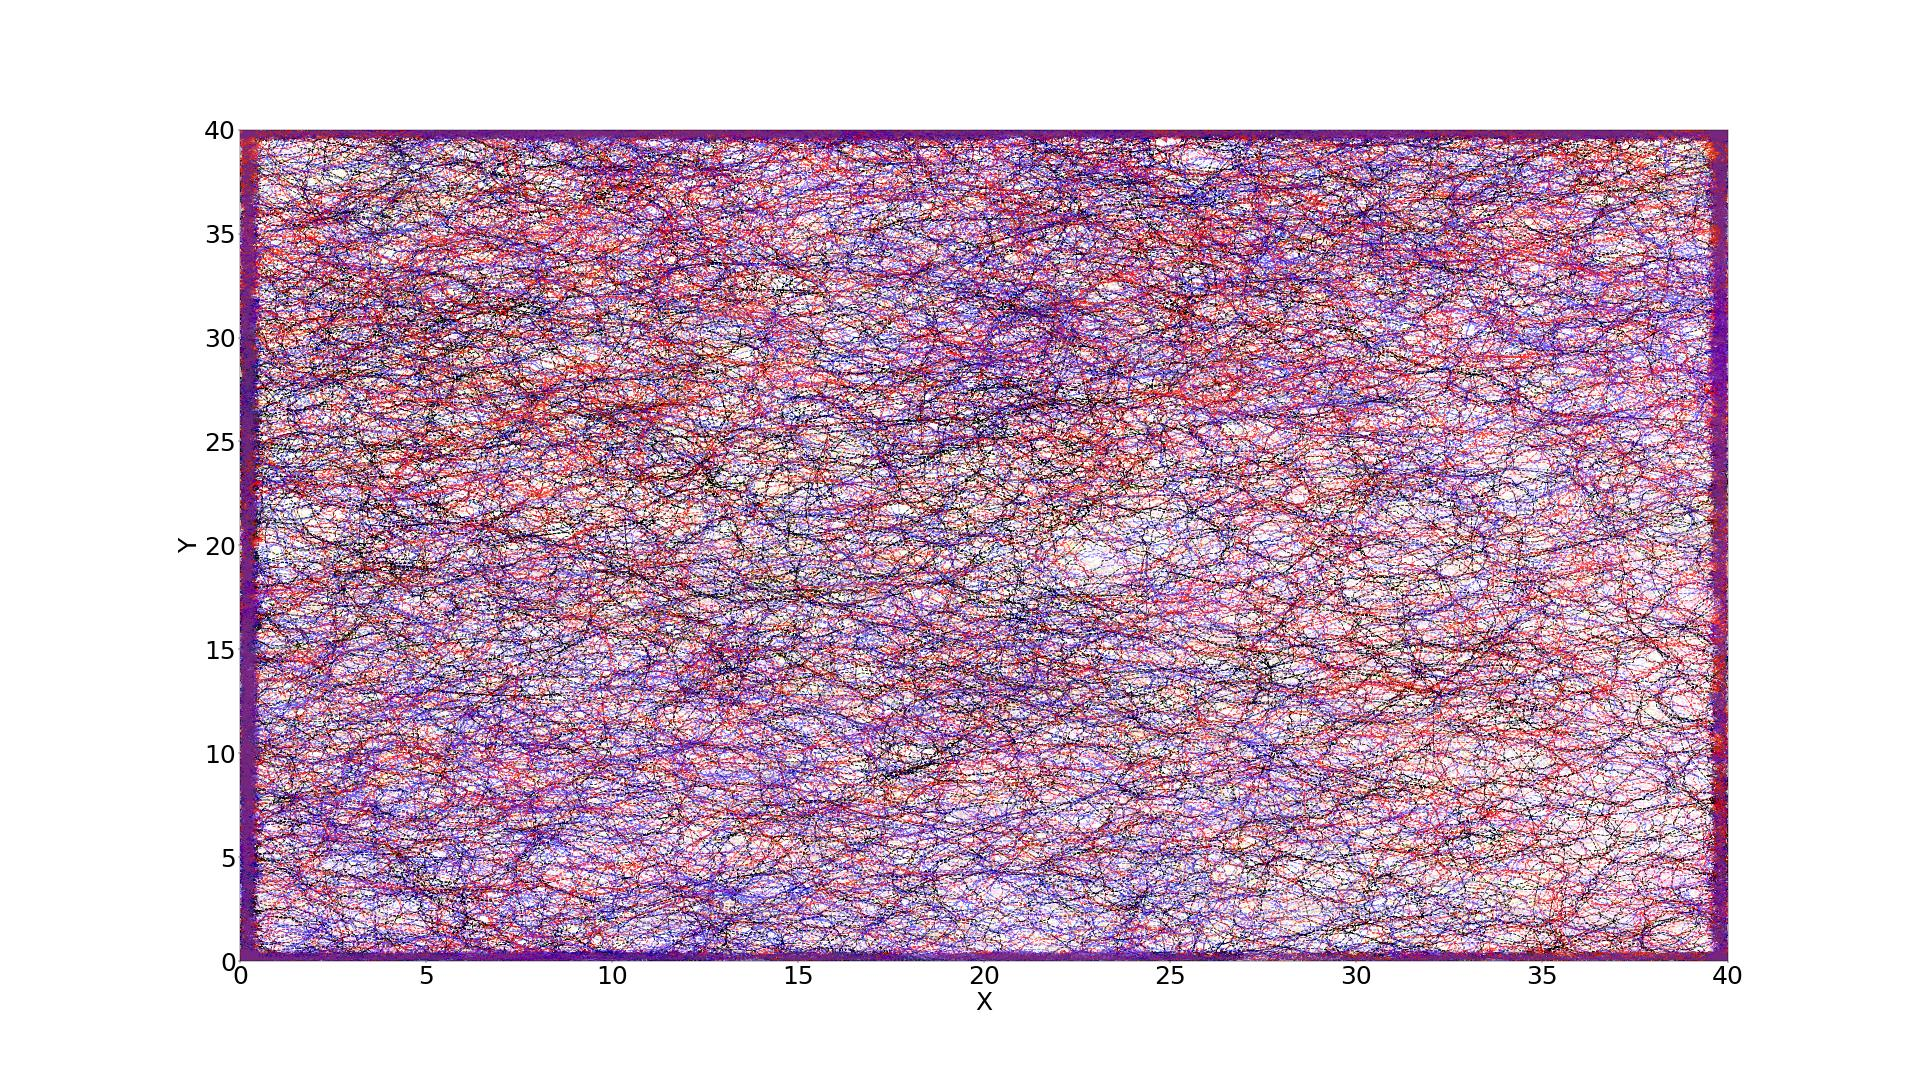
\includegraphics[width=1\linewidth]{LateX images/log/xy/g1}
	\caption{Κοινό διάγραμμα διαδρομής ρομποτικού συστήματος για, $q = -1.4$, $k = 0.75$, $(x,y) = (0.1,0.5)$ \emph{(μαύρο χρώμα)} , $(x,y) = (-0.1,0.5)$ \emph{(κόκκινο χρώμα)} , $(x,y) = (-0.1,2)$ \emph{(μπλέ χρώμα)}, $(x,y) = (0.5,1.5)$ \emph{(ροζ(magenta) χρώμα)} και $(x,y) = (0.8,1.2)$ \emph{(κίτρινο χρώμα)}.}
	\label{f:g99}	
\end{figure}

\clearpage


\section{Συμπεριφορά για Μεταβαλητό \emph{h}}
\label{sec:g4}
Για να είναι ολοκληρωμένη η μελέτη της διαδρομής του ρομποτικού συστήματος , είναι απαραίτητο να ελεχθεί ο τρόπος που αντιδράει το σύστημα στην μεταβολή της παραμέτρου \emph{h}.

Η συγκεκριμένη μελέτη χωρίστηκε σε τρείς περιπτώσεις όπου για την κάθε περίπτωση κρατούσαμε σταθερές της παραμέτρους \emph{k, q, (x,y), (X,Y)}.
Στην πρώτη περίπτωση επιλέχθηκε η παράμετρος \emph{q} να ισούται $q = -1.4$ και η παράμετρος διακλάδωσης \emph{k} να ισούται $k = 0.79$. Στην δεύτερη περίπτωση η \emph{q} ισούται $q = -1.9$ και η παράμετρος διακλάδωσης  \emph{k} να ισούται $k = 0.51$. Στην τρίτη περίπτωση η \emph{q} ισούται $q = -2.1$ και η παράμετρος διακλάδωσης  \emph{k} να ισούται $k = 0.34$.

Σε όλες τις περιπτώσεις το ρομπότ εκτέλεσε $10^5$ βήματα, ενώ η αρχική θέση του ρομποτικού συστήματος παρέμεινε σταθερή και ίση με $(X,Y) = (0,0)$, όπως και οι αρχικές συνθήκες οι οποίες ισούται με $(x,y) = (0.1,0.2)$.  Έτσι, για κάθε περίπτωση παράχθηκε το διάγραμμα της διαδρομής του ρομπότ και υπολογίστηκε το ποσοστό κάλυψης. 


\subsection{Για \emph{q = -1.4}}

Στα Σχ. \ref{f:g100}, \ref{f:g101} παρατίθενται τα διαγράμματα διαδρομής του ρομποτικού συστήματος για $q = -1.4$, $k = 0.9$ και $h =0.1$, $h =0.5$ αντίστοιχα. Tο ποσοστό κάλυψης του χώρου που προέκυψε για τις συγκεκριμένες τιμές των παραμέτρων είναι $77.1\%$, $97.4\%$ αντίστοιχα.

\begin{figure}[ht]
	\centering
	\begin{subfigure}[b]{0.55\textwidth}
		\centering
		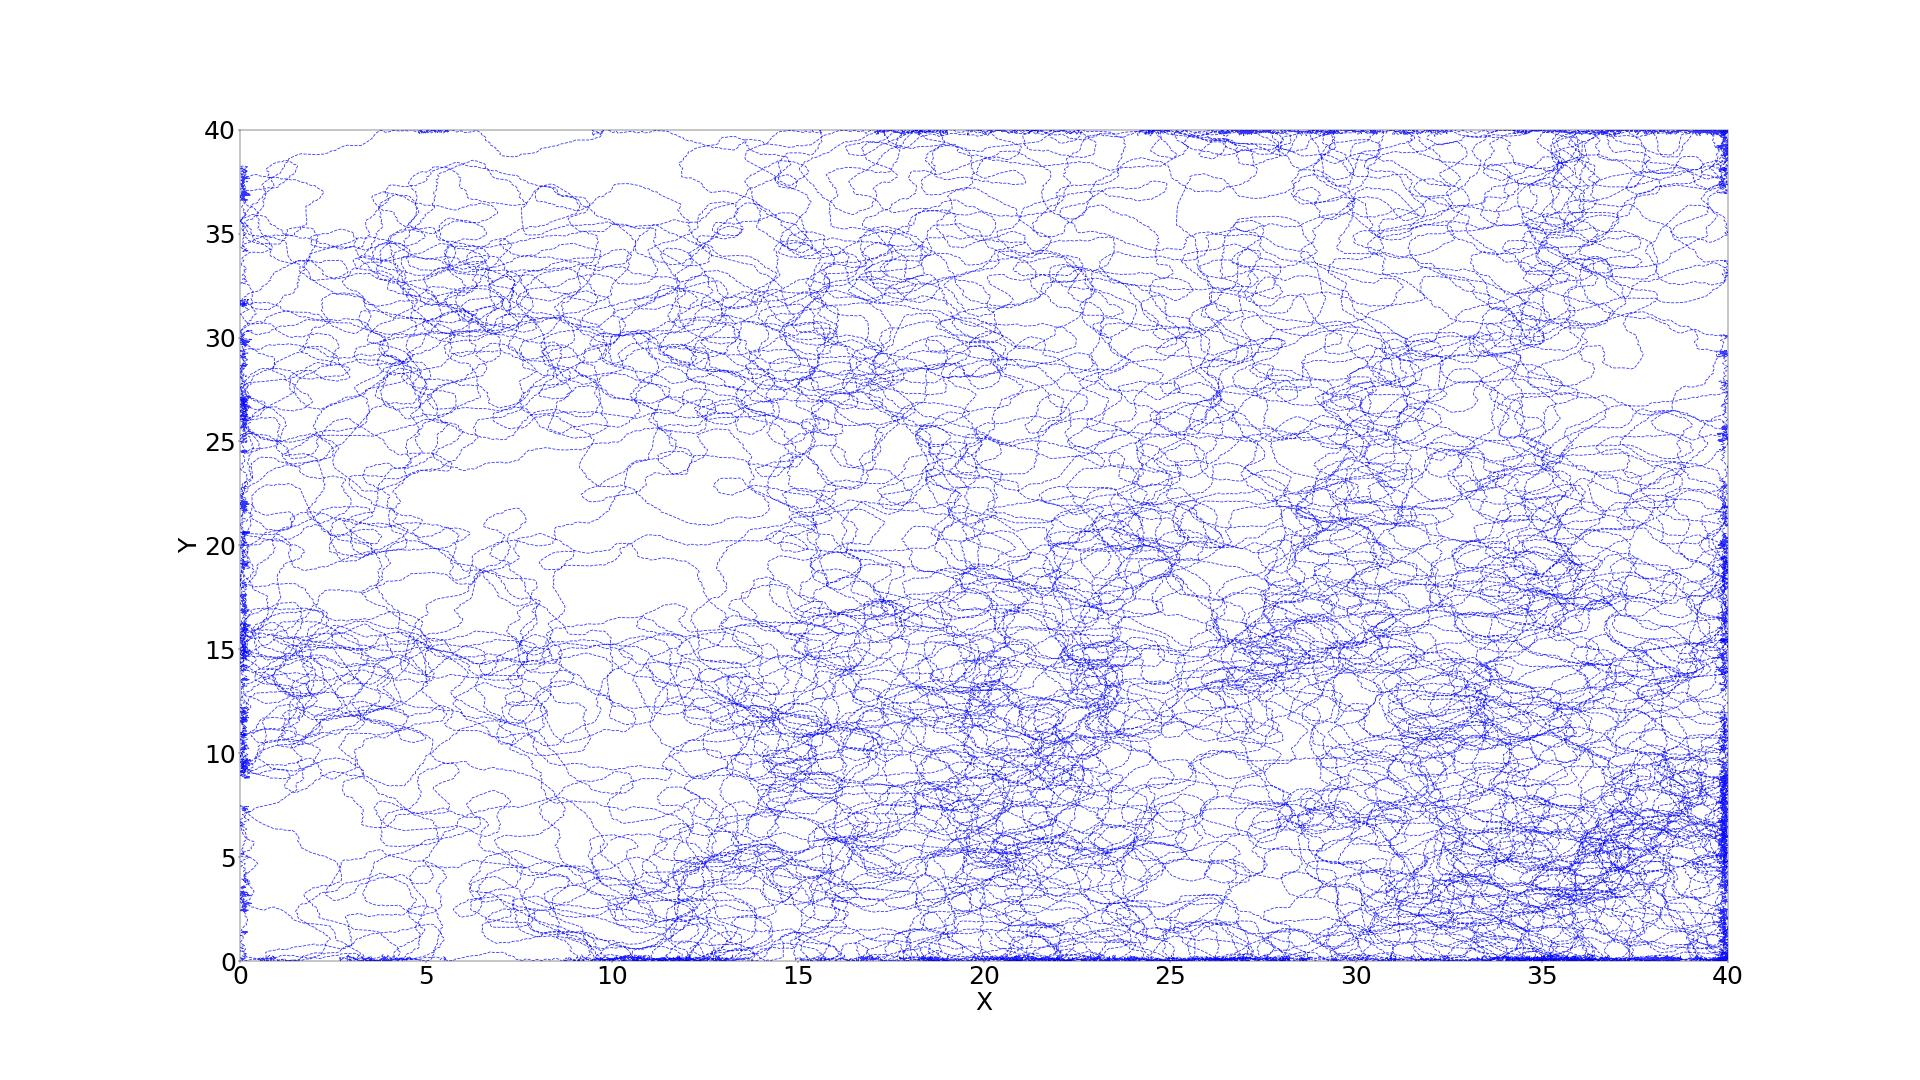
\includegraphics[width=\textwidth]{LateX images/log/h/g1-1.4}
		\caption{Για $h =0.1$.}
		\label{f:g100}
	\end{subfigure}
	\hfill
	\begin{subfigure}[b]{0.55\textwidth}
		\centering
		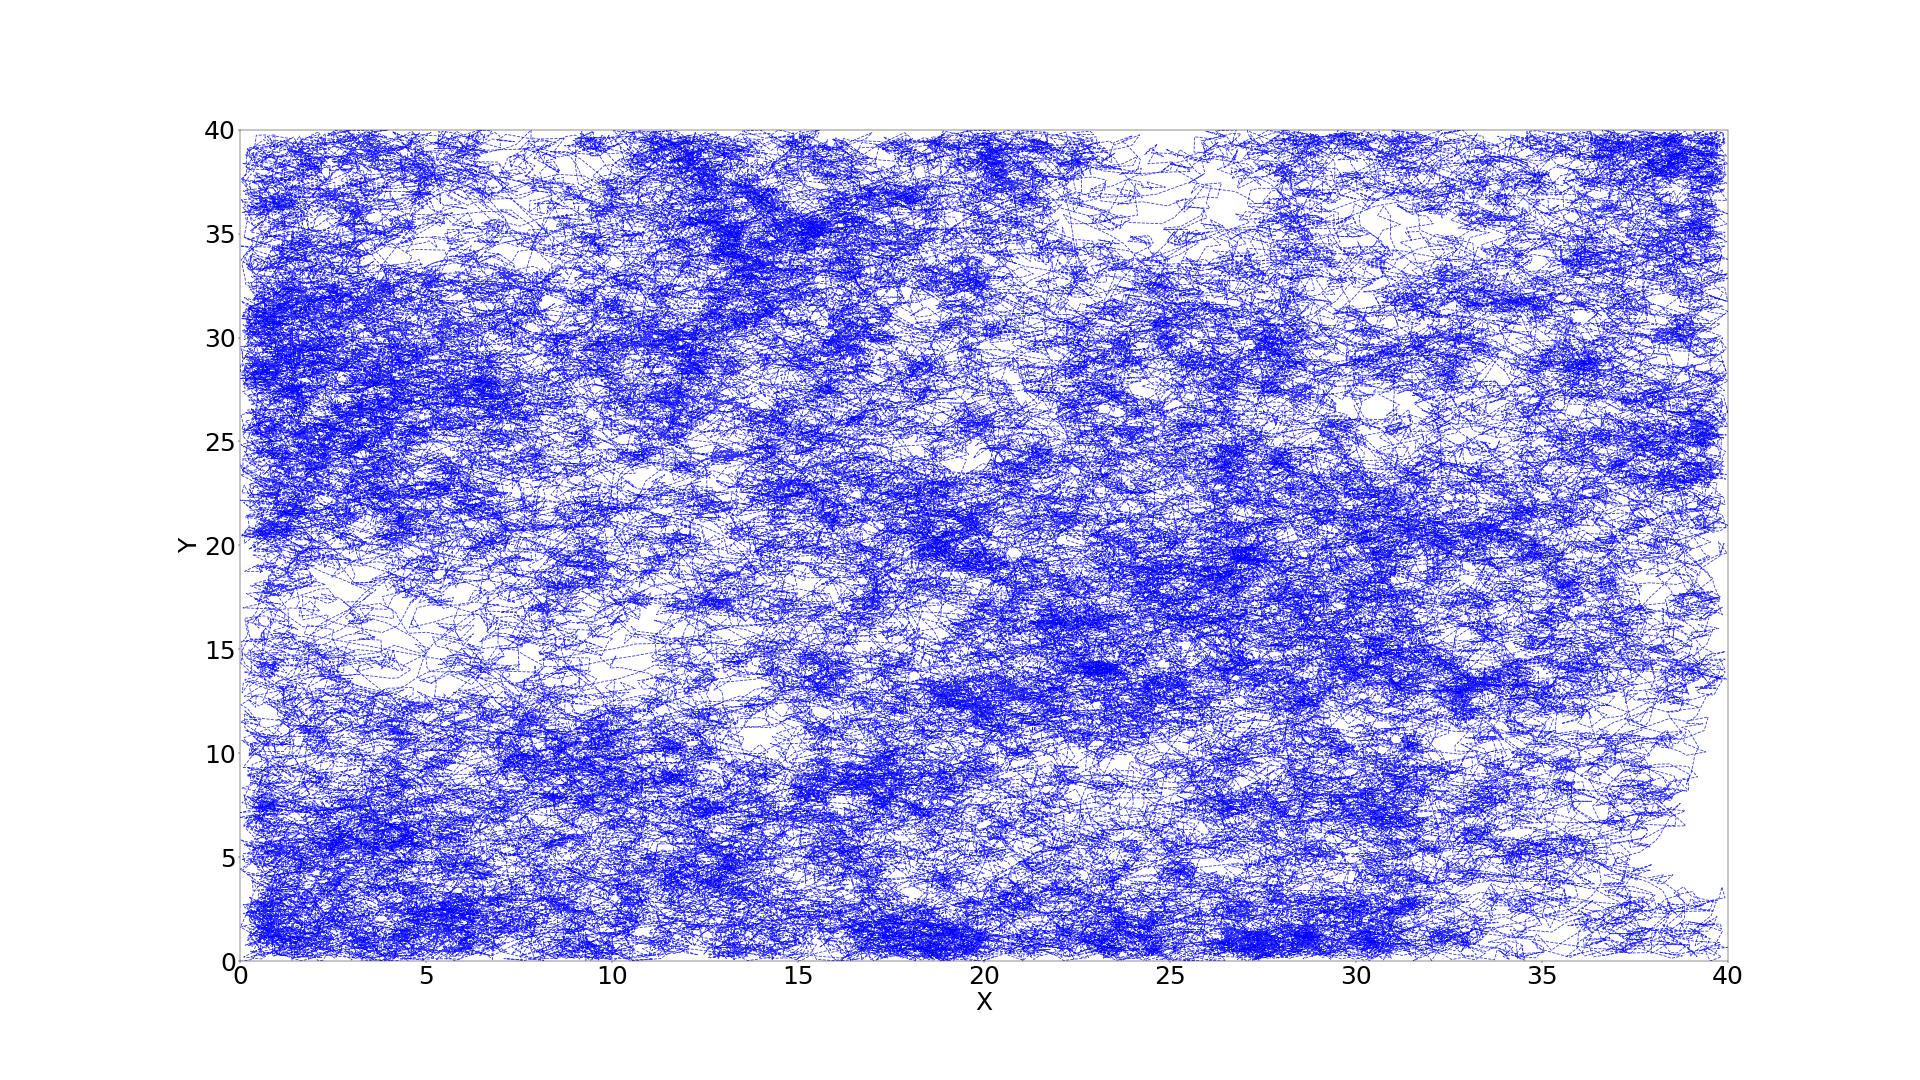
\includegraphics[width=\textwidth]{LateX images/log/h/g2-1.4}
		\caption{Για $h =0.5$.}
		\label{f:g101}
	\end{subfigure}
	\hfill
\caption{Διαγράμματα διαδρομής ρομποτικού συστήματος για, $q = -1.4$, $k = 0.79$ και :}
\end{figure}

\clearpage
\subsection{Για \emph{q = -1.9}}

Στα Σχ. \ref{f:g102}, \ref{f:g103} παρατίθενται τα διαγράμματα διαδρομής του ρομποτικού συστήματος για $q = -1.9$, $k = 0.51$ και $h =0.1$, $h =0.5$ αντίστοιχα. Tο ποσοστό κάλυψης του χώρου που προέκυψε για τις συγκεκριμένες τιμές των παραμέτρων είναι $60.1\%$, $99.9\%$ αντίστοιχα.

\begin{figure}[ht]
	\centering
	\begin{subfigure}[b]{0.55\textwidth}
		\centering
		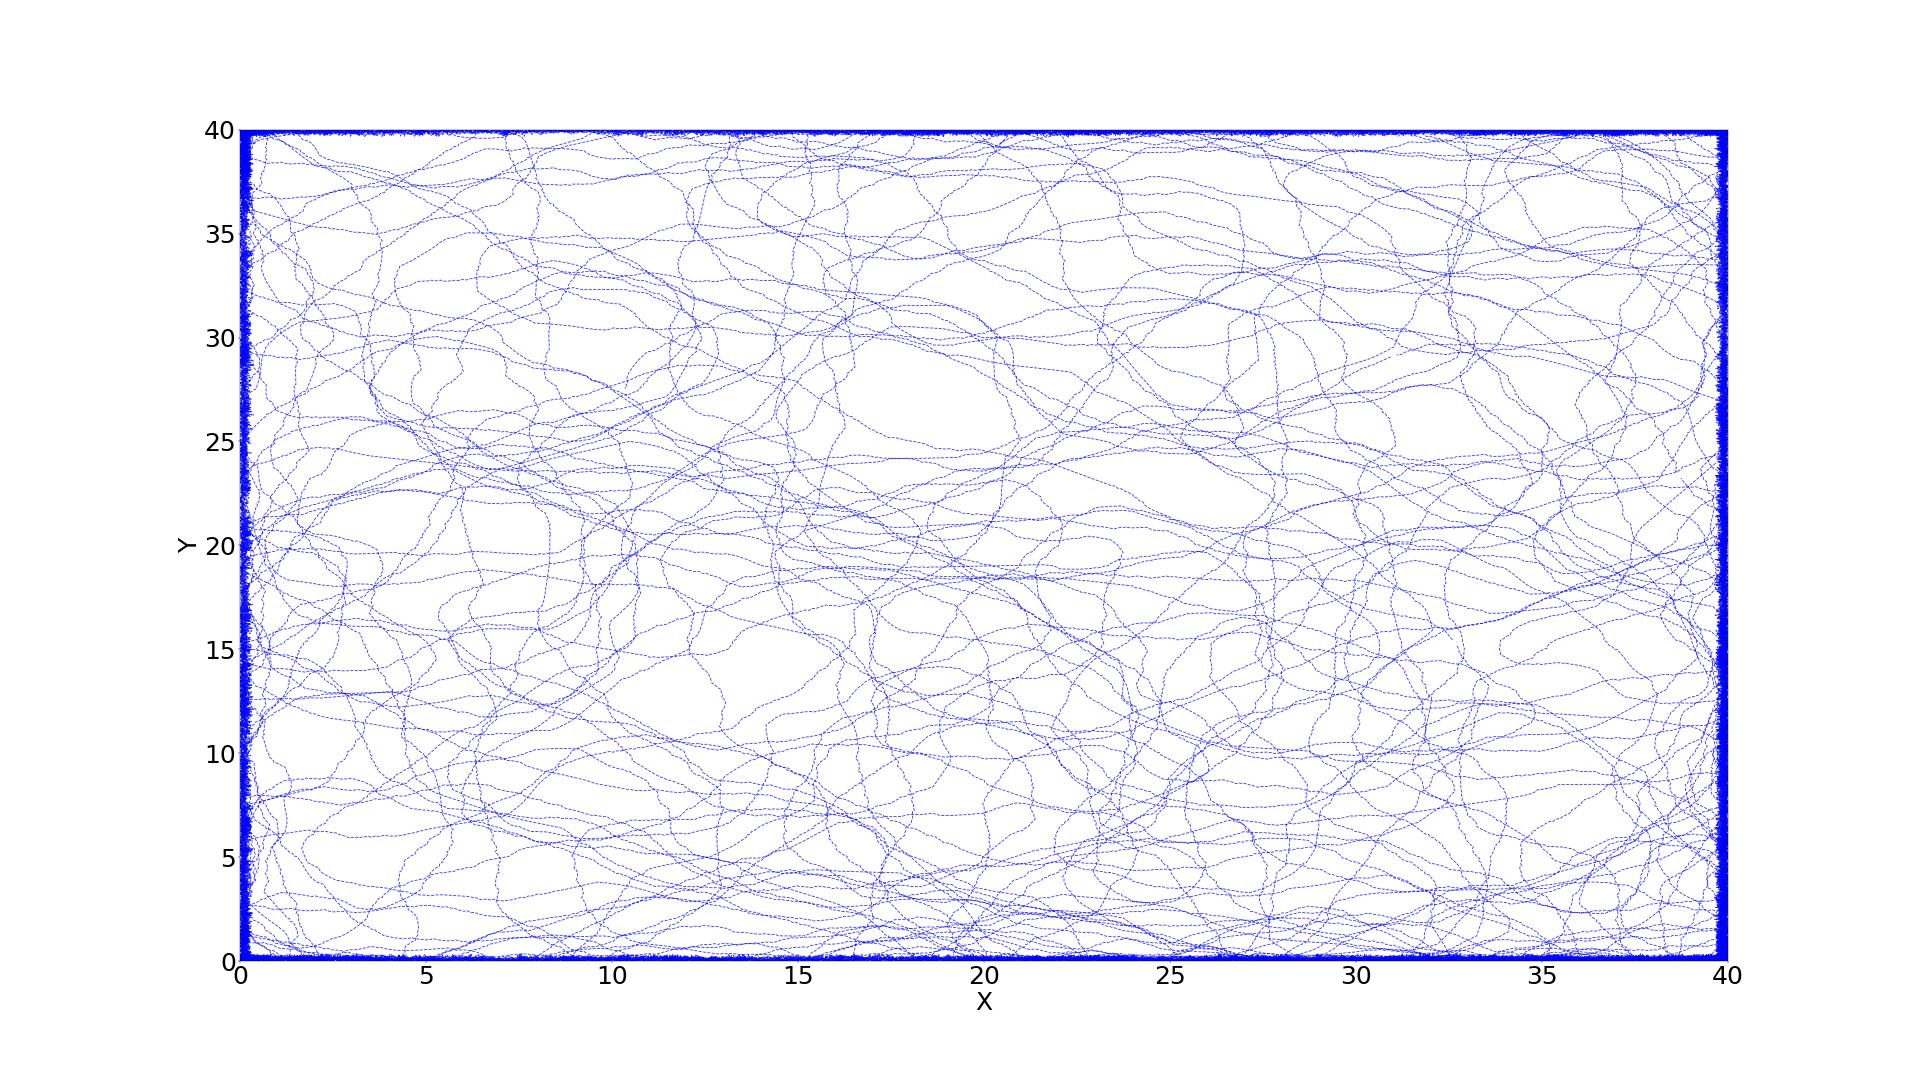
\includegraphics[width=\textwidth]{LateX images/log/h/g1-1.9}
		\caption{Για $h =0.1$.}
		\label{f:g102}
	\end{subfigure}
	\hfill
	\begin{subfigure}[b]{0.55\textwidth}
		\centering
		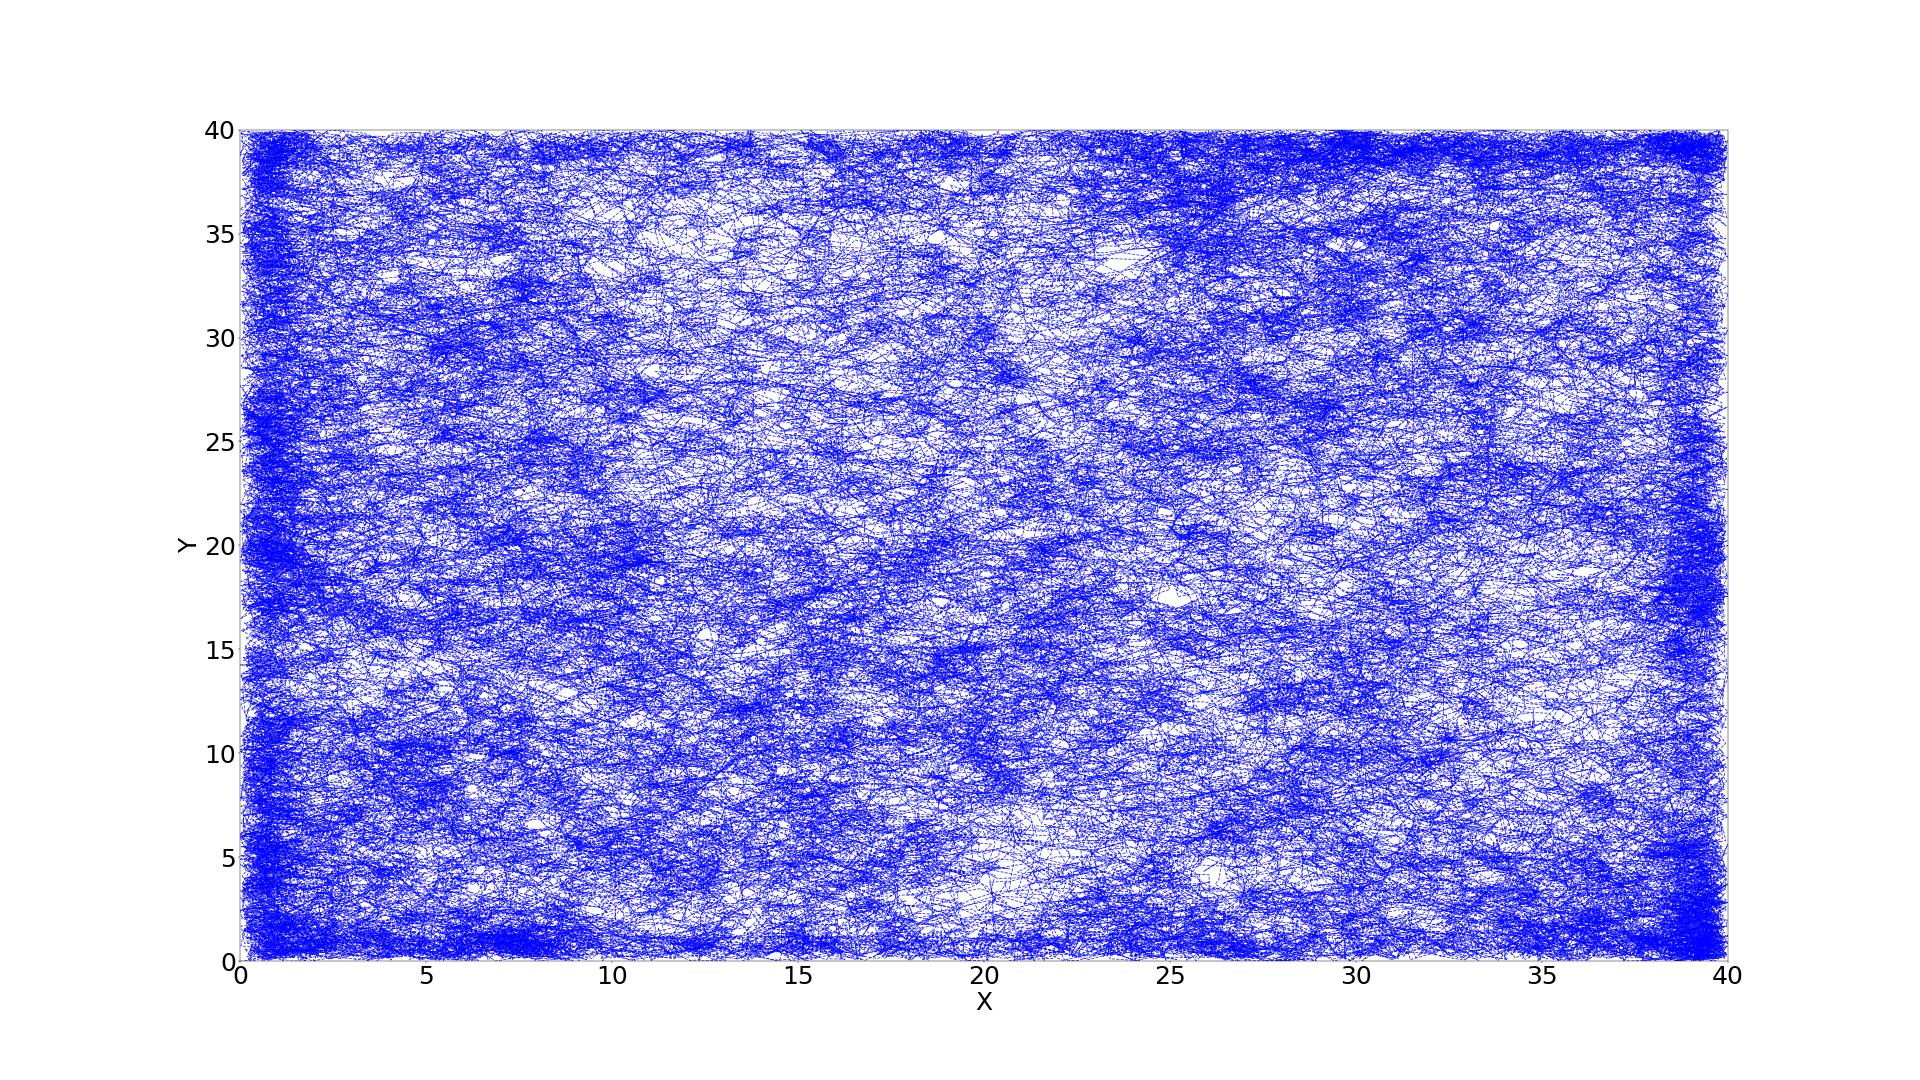
\includegraphics[width=\textwidth]{LateX images/log/h/g2-1.9}
		\caption{Για $h =0.5$.}
		\label{f:g103}
	\end{subfigure}
	\hfill
	\caption{Διαγράμματα διαδρομής ρομποτικού συστήματος για, $q = -1.9$, $k = 0.51$ και :}
\end{figure}

\clearpage

\subsection{Για \emph{q = -2.1}}

Στα Σχ. \ref{f:g104}, \ref{f:g105}, \ref{f:g106}, \ref{f:g107} παρατίθενται τα διαγράμματα διαδρομής του ρομποτικού συστήματος για $q = -2.1$, $k = 0.34$ και $h =0.1$, $h =0.5$, $h =0.8$, $h =1.2$ αντίστοιχα.Tο ποσοστό κάλυψης του χώρου που προέκυψε για τις συγκεκριμένες τιμές των παραμέτρων είναι $2.27\%$, $18.3\%$, $34.03\%$, $57.8\%$ αντίστοιχα.


\begin{figure}[ht]
\centering
\begin{subfigure}[b]{0.55\textwidth}
	\centering
	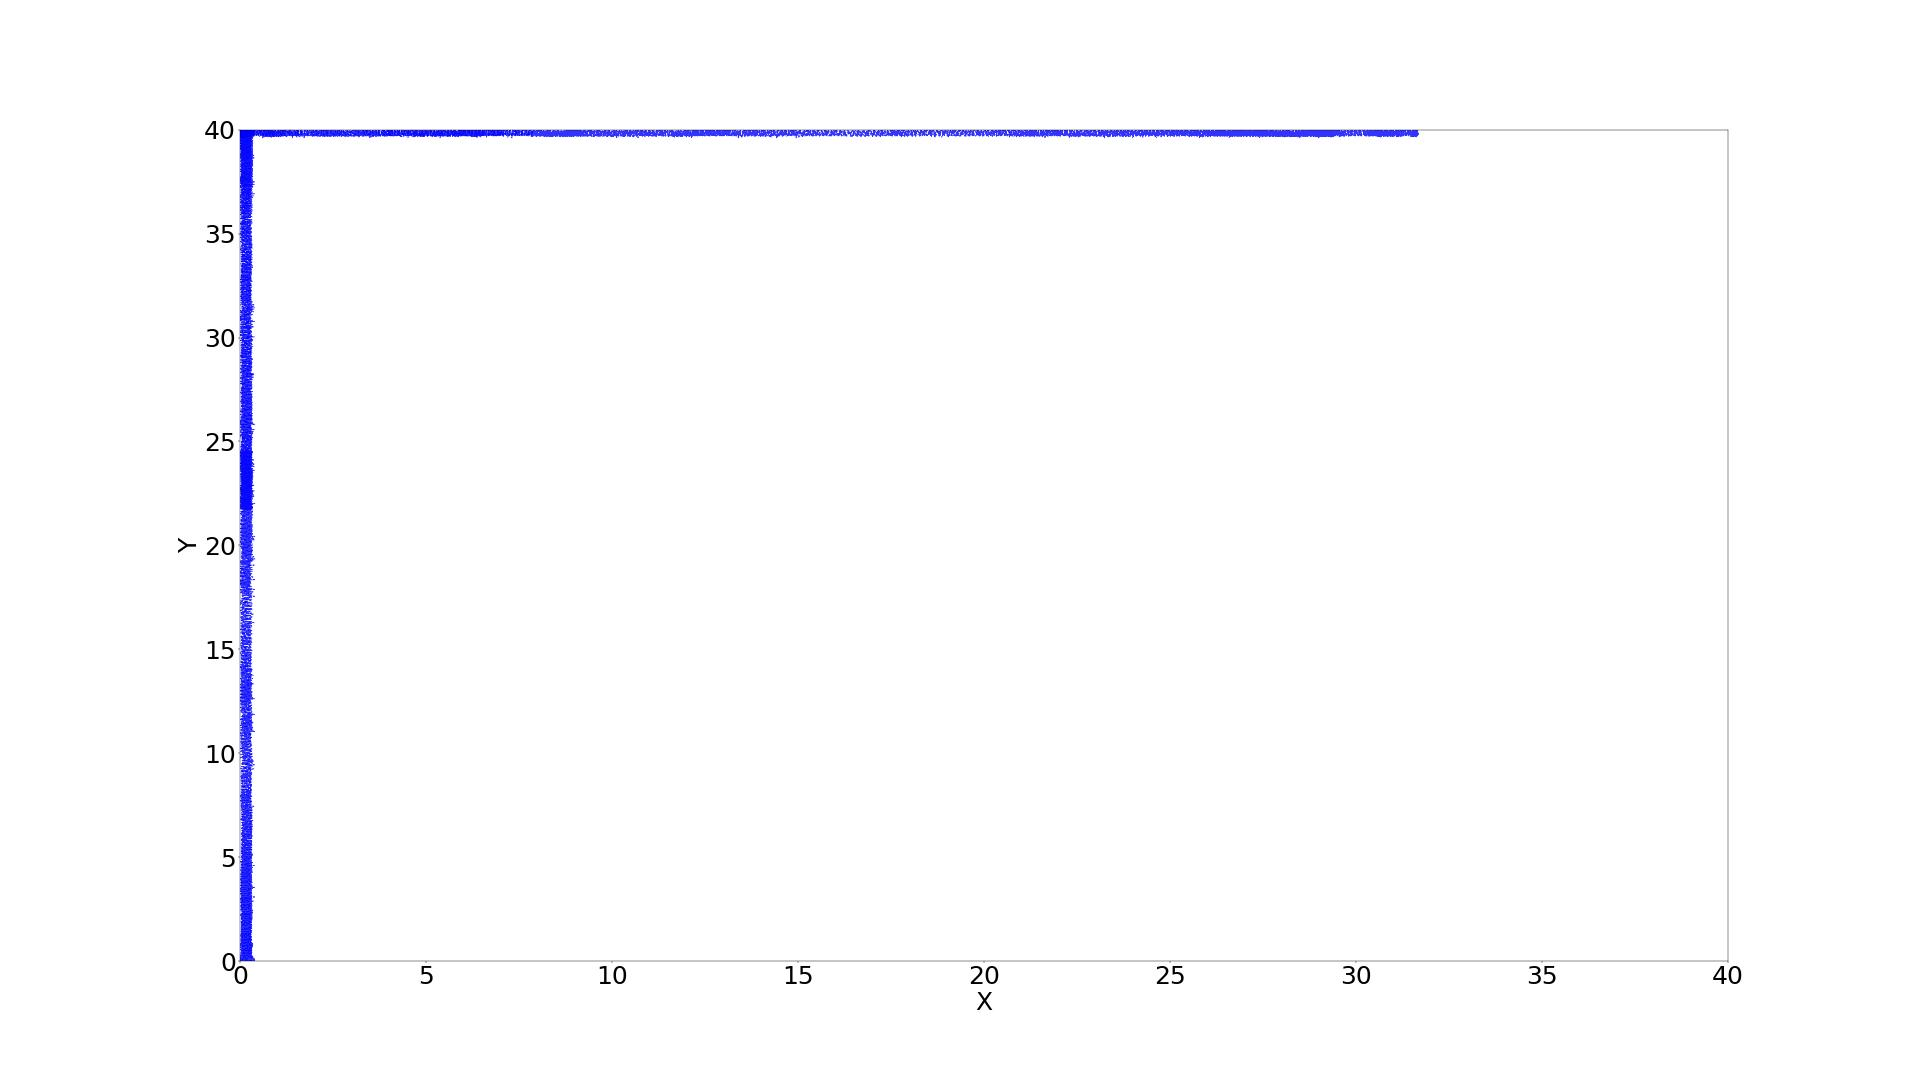
\includegraphics[width=\textwidth]{LateX images/log/h/g1-2.1}
	\caption{Για $h =0.1$.}
	\label{f:g104}
\end{subfigure}
\hfill
\begin{subfigure}[b]{0.55\textwidth}
	\centering
	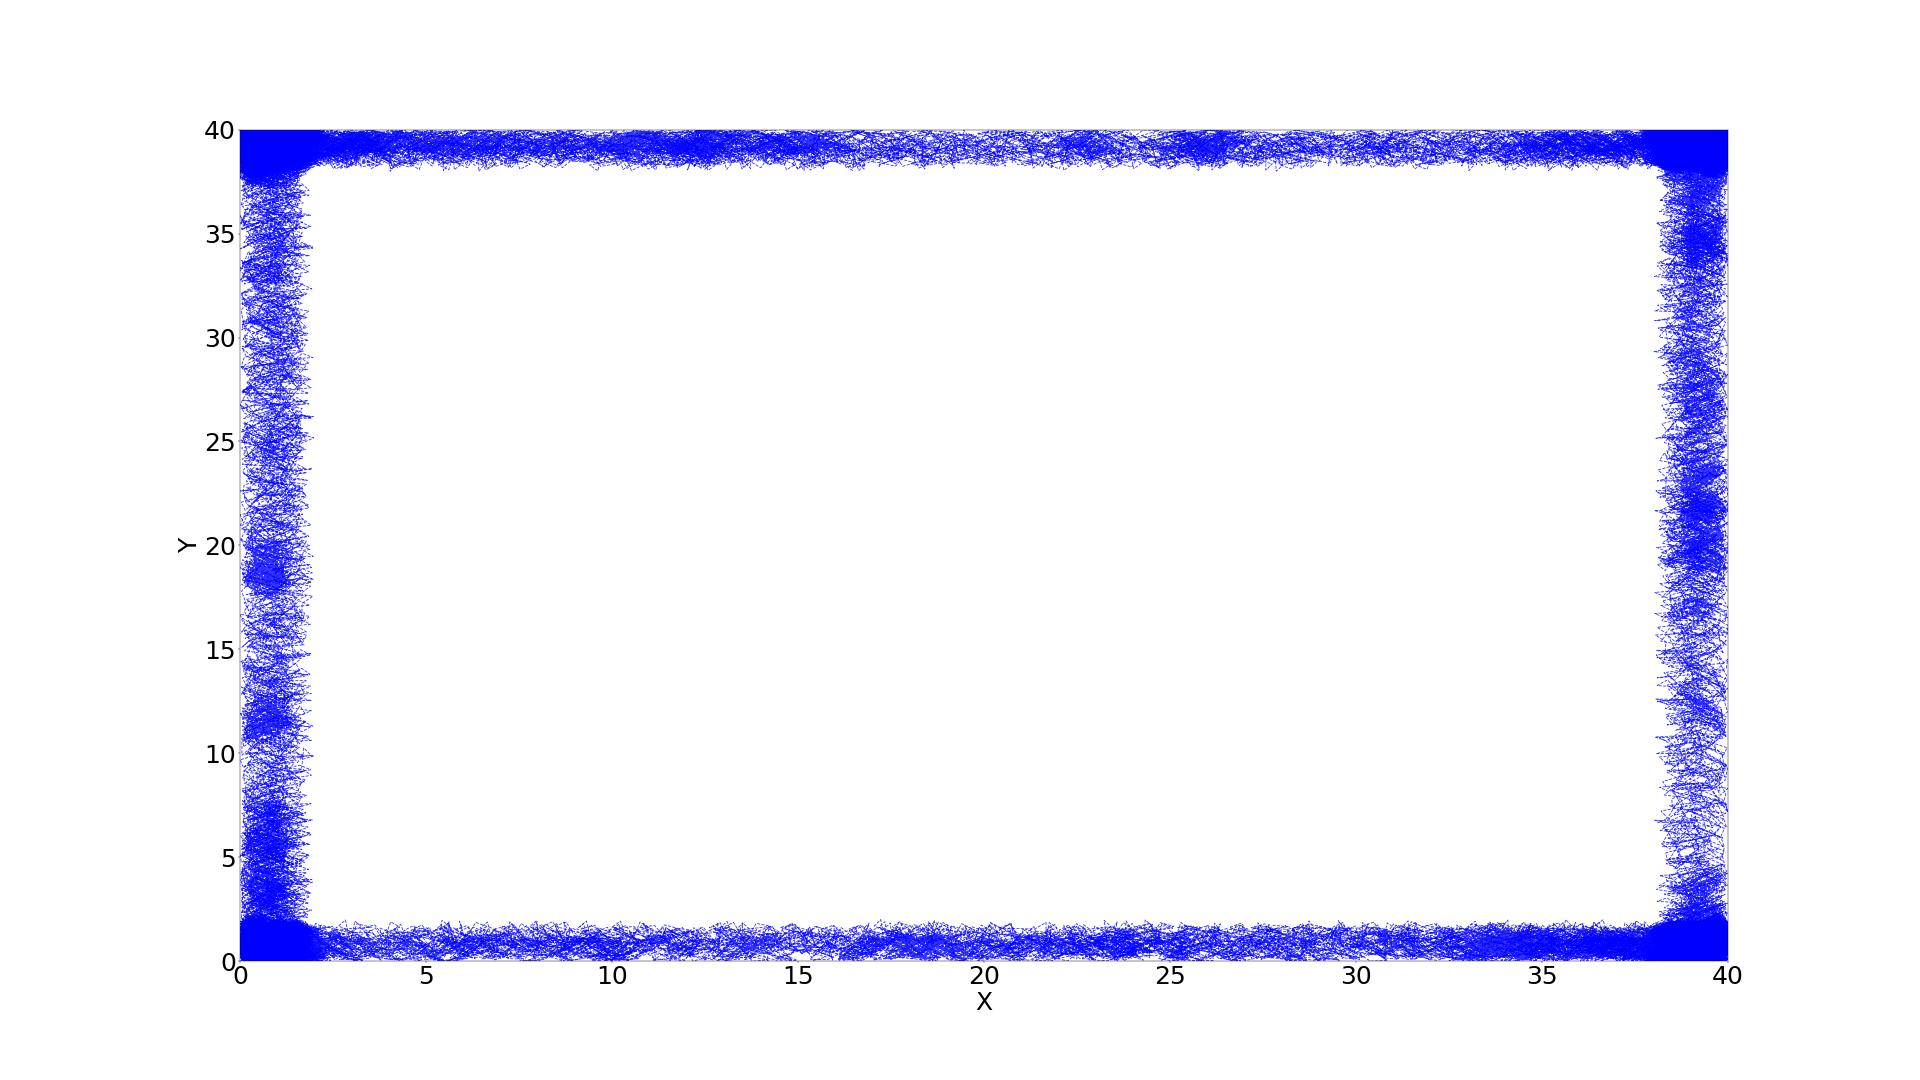
\includegraphics[width=\textwidth]{LateX images/log/h/g2-2.1}
	\caption{Για $h =0.5$.}
	\label{f:g105}
\end{subfigure}
\hfill
\begin{subfigure}[b]{0.55\textwidth}
	\centering
	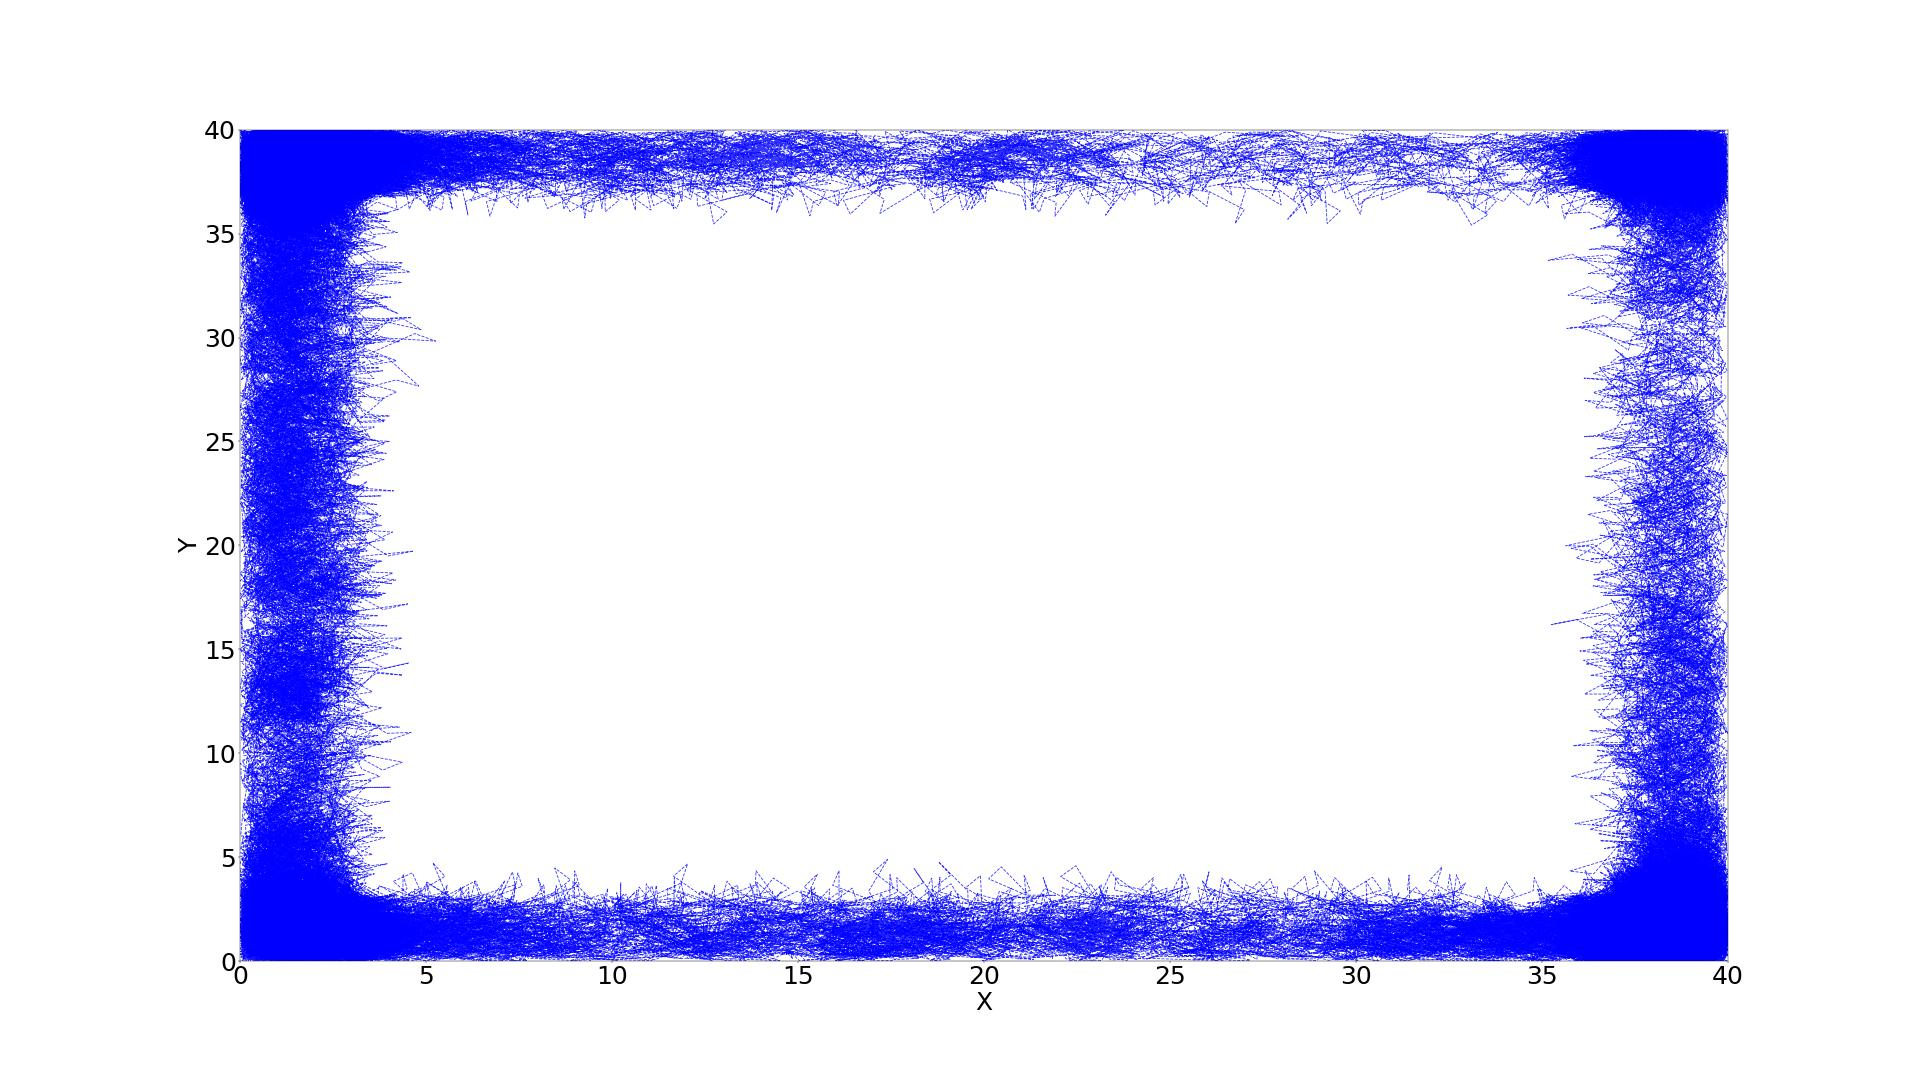
\includegraphics[width=\textwidth]{LateX images/log/h/g3-2.1}
	\caption{Για $h =0.8$.}
	\label{f:g106}
\end{subfigure}
\hfill
\begin{subfigure}[b]{0.55\textwidth}
	\centering
	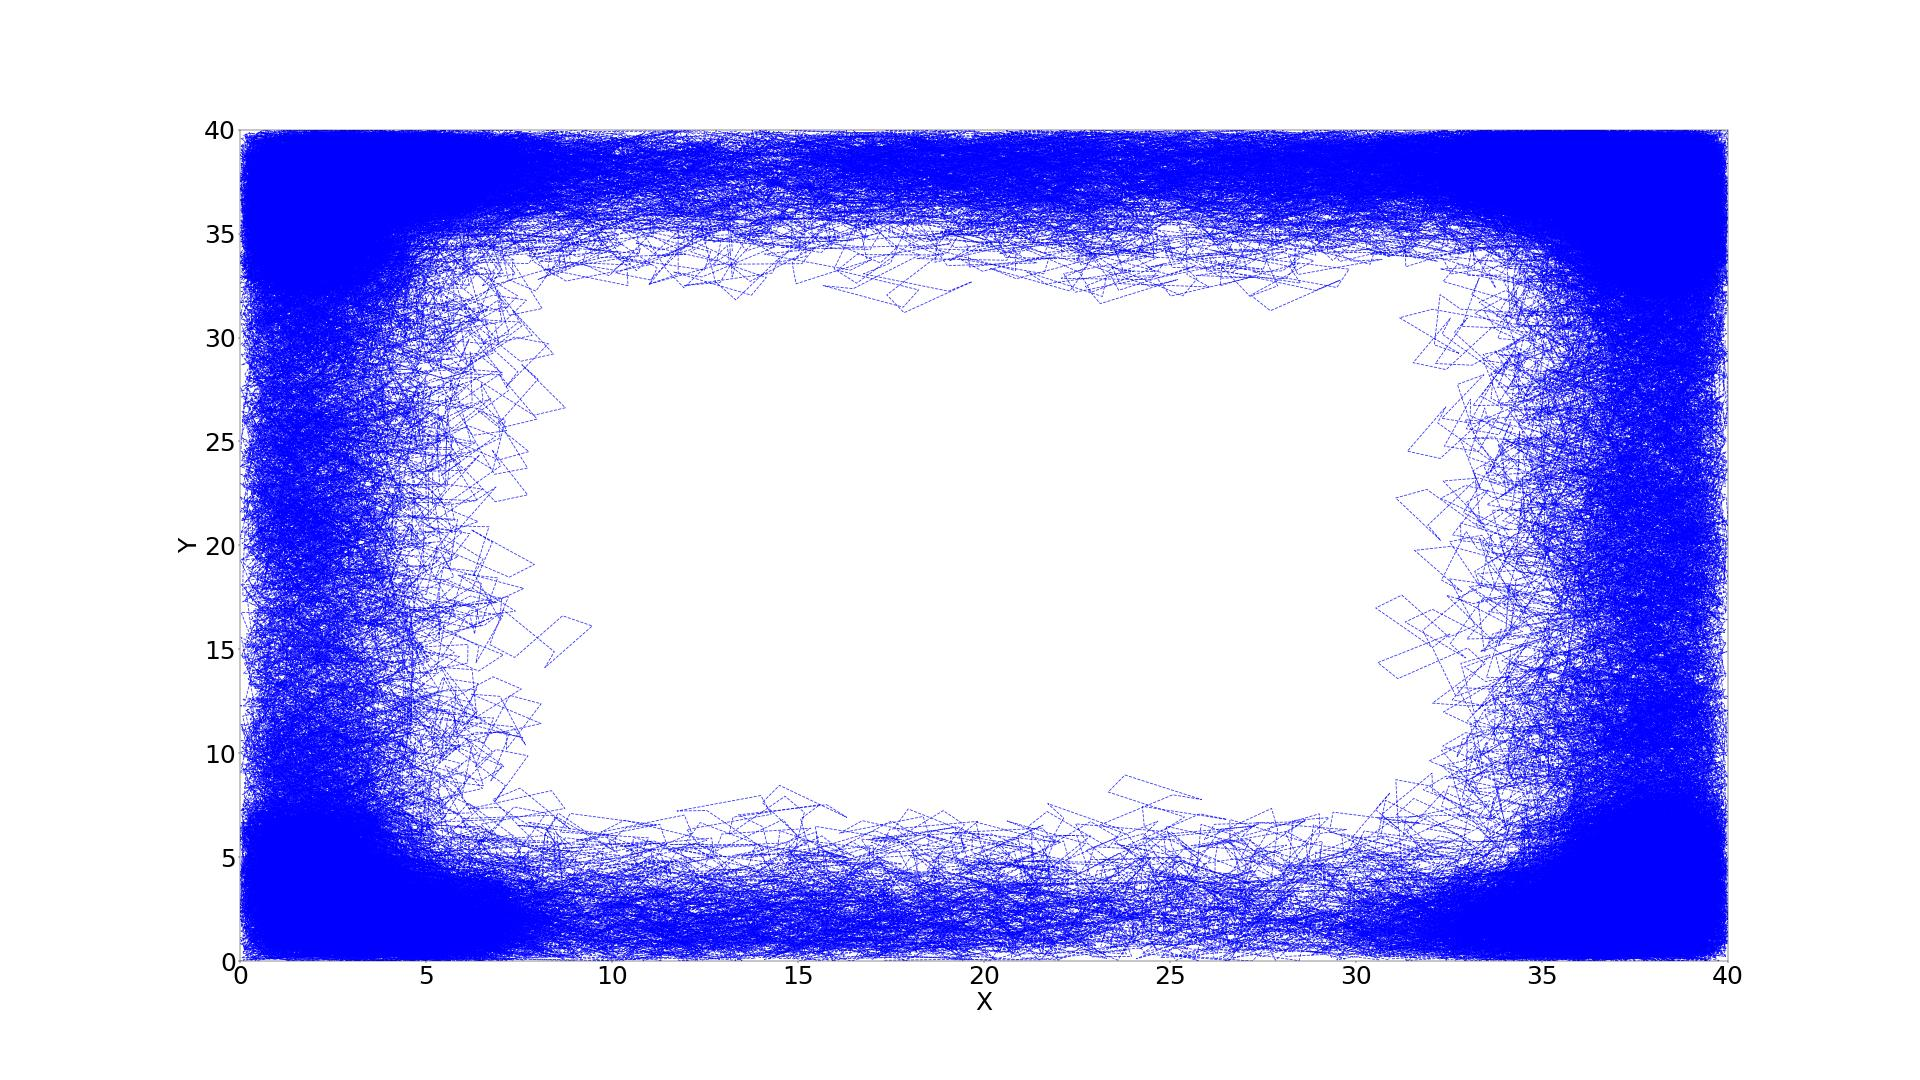
\includegraphics[width=\textwidth]{LateX images/log/h/g4-2.1}
	\caption{Για $h =1.2$.}
	\label{f:g107}
\end{subfigure}
\hfill
\caption{Διαγράμματα διαδρομής ρομποτικού συστήματος για, $q = -2.1$, $k = 0.34$ και :}
\end{figure}

Από τα παραπάνω διαγράμματα παρατηρείται ότι αλλάζοντας ελάχιστα την παράμετρο διακριτοποίησης \emph{h} έχει ως συνέπεια να μεταβληθεί σημαντικά το ποσοστό κάλυψης που παρουσιάζει η εκάστοτε κίνηση. Αναλυτικότερα, όσο πιο μικρή είναι η τιμή του \emph{h} τόσο μικρότερη θα είναι η καλυψιμότητα του χώρου που κινείται το ρομπότ, ενώ αν την αυξήσουμε αρκετά μετά από ένα σημείο αλλάζει ελάχιστα εφόσον έχει φτάσει σχεδόν στο $100\%$. Αυτό μπορεί να παρατηρηθεί στην δεύτερη περίπτωση για $q = -1.9$ όπου μετά απο $h = 0.5$ θα αρχίσουμε να παρατηρούμε όλο και μικρότερη αύξηση του ποσοστού κάλυψης της επιφάνειας. Παρόλο που δεν υπάρχει κάποιο διάγραμμα , για παράδειγμα για $h - 0.6$ και για $h = 0.8$ το ποσοστό κάλύψεις είναι $99.93\%$,  $99.96\%$ αντίστοιχα. Δηλαδή μέσα σε $0.4$ βήματα του \emph{h} το ποσοστό ανέβηκε περίπου μόνο \textbf{0.04} μονάδες.

\clearpage

\section{Συμπεριφορά για Μεταβαλλόμενο Αριθμό Βημάτων}
\label{sec:g5}
Ολοκληρώνοντας την μελέτη της διαδρομής που ακολουθεί το ρομποτικό
σύστημα, ερευνάται η συμπεριφορά του συστήματος όταν μεταβάλλεται ο αριθμός βημάτων. Για τον σκοπό αυτό θα αναλυθεί και θα υπολογιστεί το ποσοστό κάλυψης για ένα εύρος βημάτων ανάλογα την περίπτωση. Ελέχθηκαν δύο περιπτώσεις στις οποίες είναι σταθερές όλες οι παράμετροι. Στην πρώτη περίπτωση για $q = -1.6$ και $k = 0.79$ το εύρος βήμάτων ήταν μεταξύ $(10^5-10^7)$ με τυχαίο βήμα.
Στην δεύτερη περίπτωση για $q = -1.9$ και $k = 0.68$ το εύρος βήμάτων ήταν μεταξύ $(10^4-10^6)$ εξίσου με τυχαίο βήμα.

Σε όλες τις περιπτώσεις η παράμετρος διακριτοποίησης \emph{h} παρέμεινε σταθερή και ίση με $h = 0.2$ ,η αρχική θέση του ρομποτικού συστήματος παρέμεινε σταθερή και ίση με $(X,Y) = (0,0)$, όπως και οι αρχικές συνθήκες οι οποίες ισούται με $(x,y) = (0.1,0.2)$.  Έτσι, για κάθε περίπτωση παράχθηκε ένας πίνακας με τους αριθμούς βημάτων και τα ποσοστά κάλυψης.

\subsection{Για \emph{q = -1.6}}

Σύμφωνα με τα δεδομένα του πίνακα \ref{tab:abc14} κατασκευάστηκε διάγραμμα του αριθμού των βημάτων που εκτελεί το ρομπότ συναρτήσει του ποσοστού κάλυψης. Όπως φαίνεται στο Σχ. \ref{f:g108} η μεταβολή της συναρτησιακής αυτής σχέσης είναι κατά προσέγγιση εκθετική. Στα Σχ. \ref{f:g109}, \ref{f:g110}, \ref{f:g111} παρουσιάζονται τα διαγράμματα διαδρομής ρομποτικού συστήματος, για αριθμό βημάτων $10^5$, $10^6$ και $5*10^6$ αντίστοιχα.

\begin{table}[ht]
	\centering
	\caption{Συμπεριφορά του υπό μελέτη συστήματος για διαφορετικό αριθμό βημάτων και για $q = -1.6$, $k = 0.79$.}
	\begin{tabular}{l | l }
		Αριθμός Βημάτων & Ποσοστό Κάλυψης \\

		$10^5$ &  $10.46$ \\
		$5*10^5$ & $19.6$ \\
		$7*10^5$&  $23.2$ \\
		$10^6$ & $25.57$ \\
		$5*10^6$& $51.25$\\
		$10^7$& $63.8$ \\
	
	\end{tabular}	
	\label{tab:abc14}
\end{table}




\begin{figure}[ht]
	\centering
	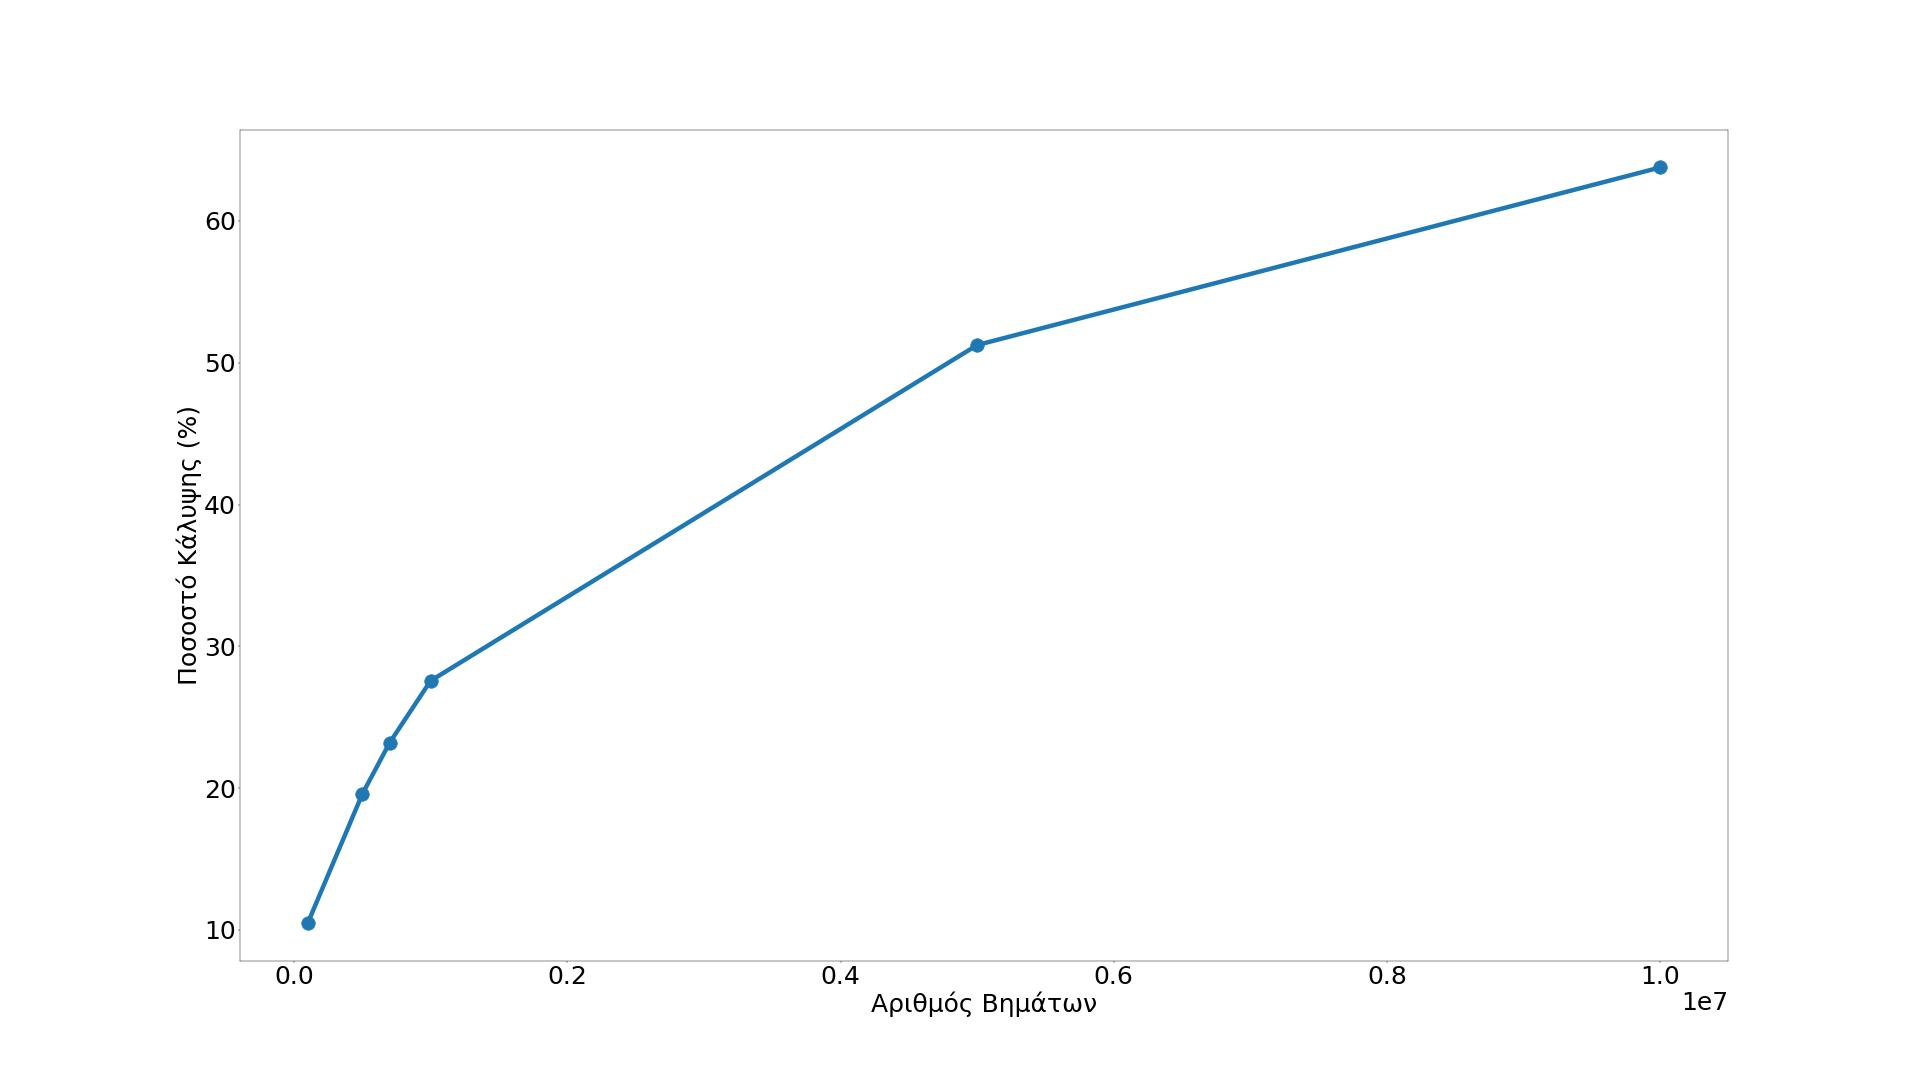
\includegraphics[width=1\linewidth]{LateX images/log/steps/g1}
	\caption{Διάγραμμα μεταβολής του ποσοστού κάλυψης συναρτήσει του αριθμού βημάτων για $q = -1.6$ και $k= 0.79$.}
	\label{f:g108}	
\end{figure}

\begin{figure}[ht]
\centering
\begin{subfigure}[b]{0.75\textwidth}
	\centering
	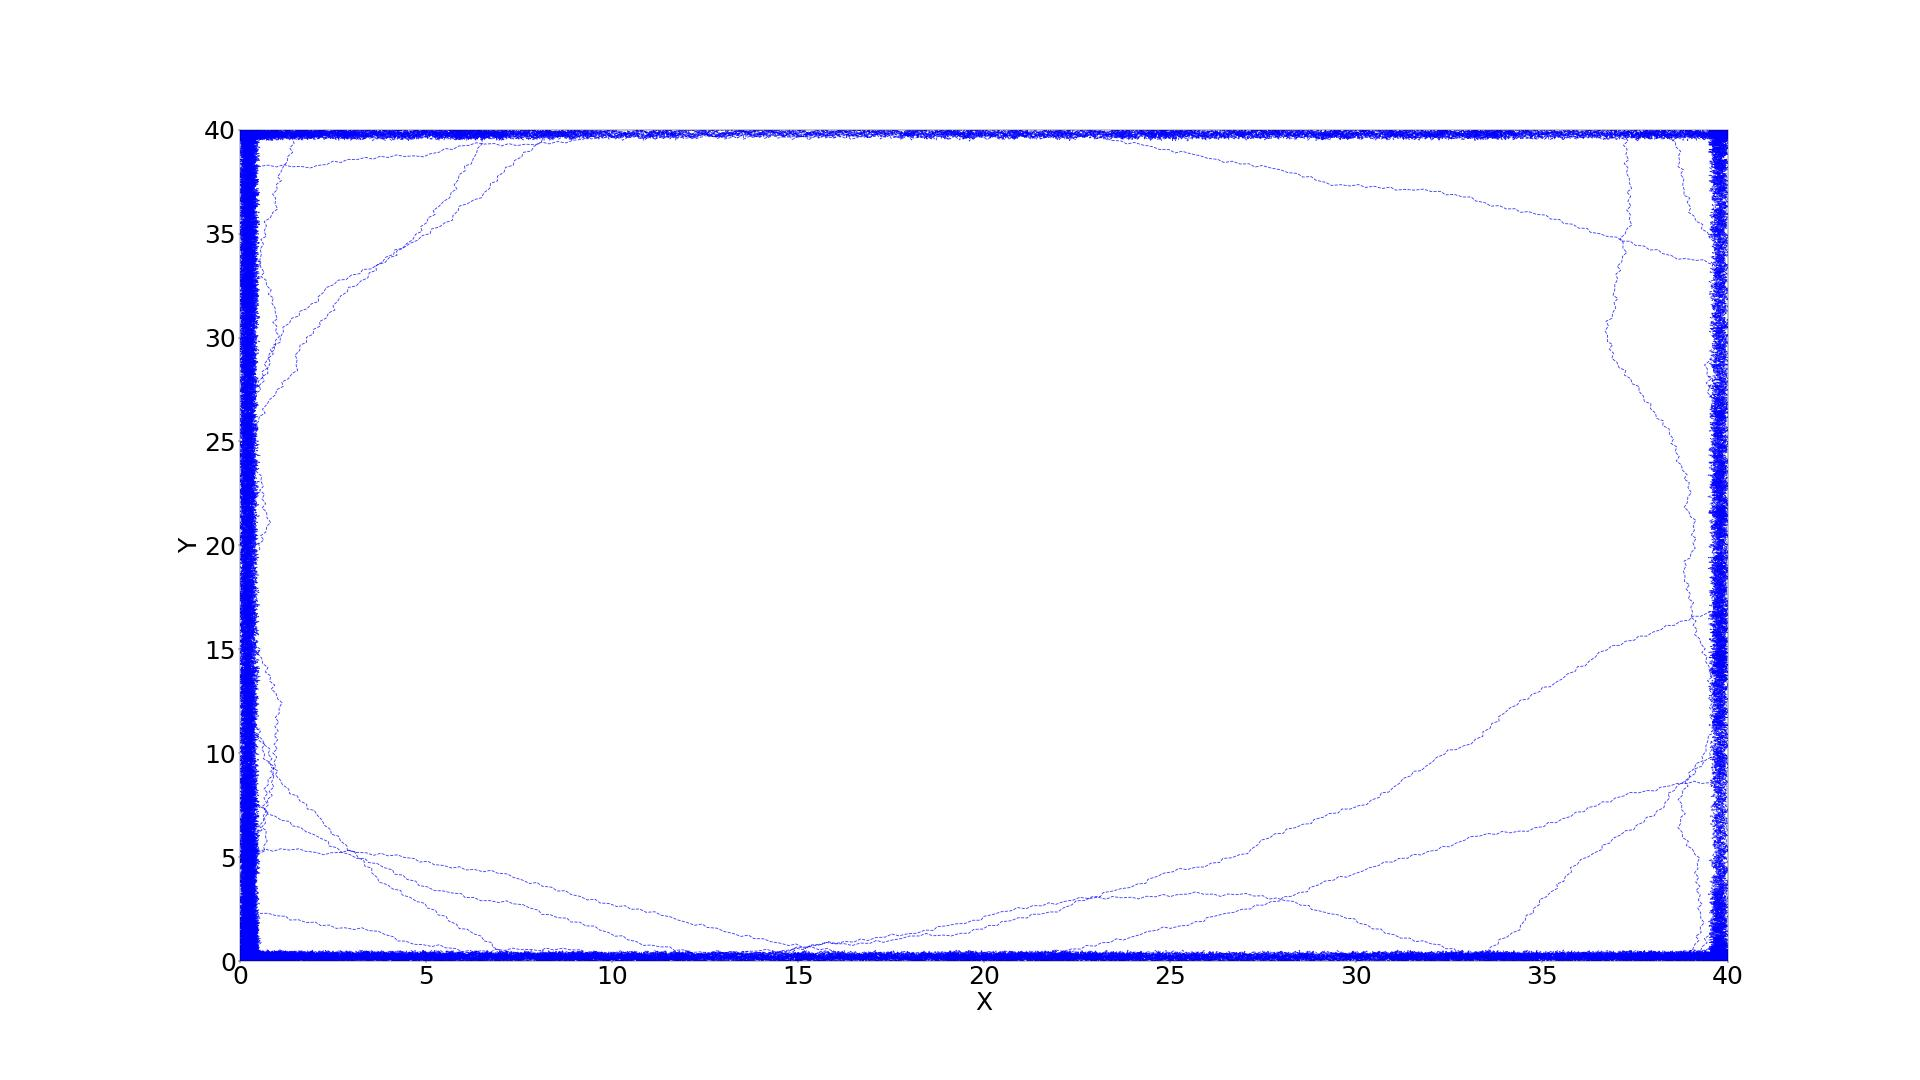
\includegraphics[width=\textwidth]{LateX images/log/steps/g3-1.6}
	\caption{Αριθμό βημάτων $10^5$ και ποσοστό κάλυψης $10.46$.}
	\label{f:g109}
\end{subfigure}
\hfill
\begin{subfigure}[b]{0.75\textwidth}
	\centering
	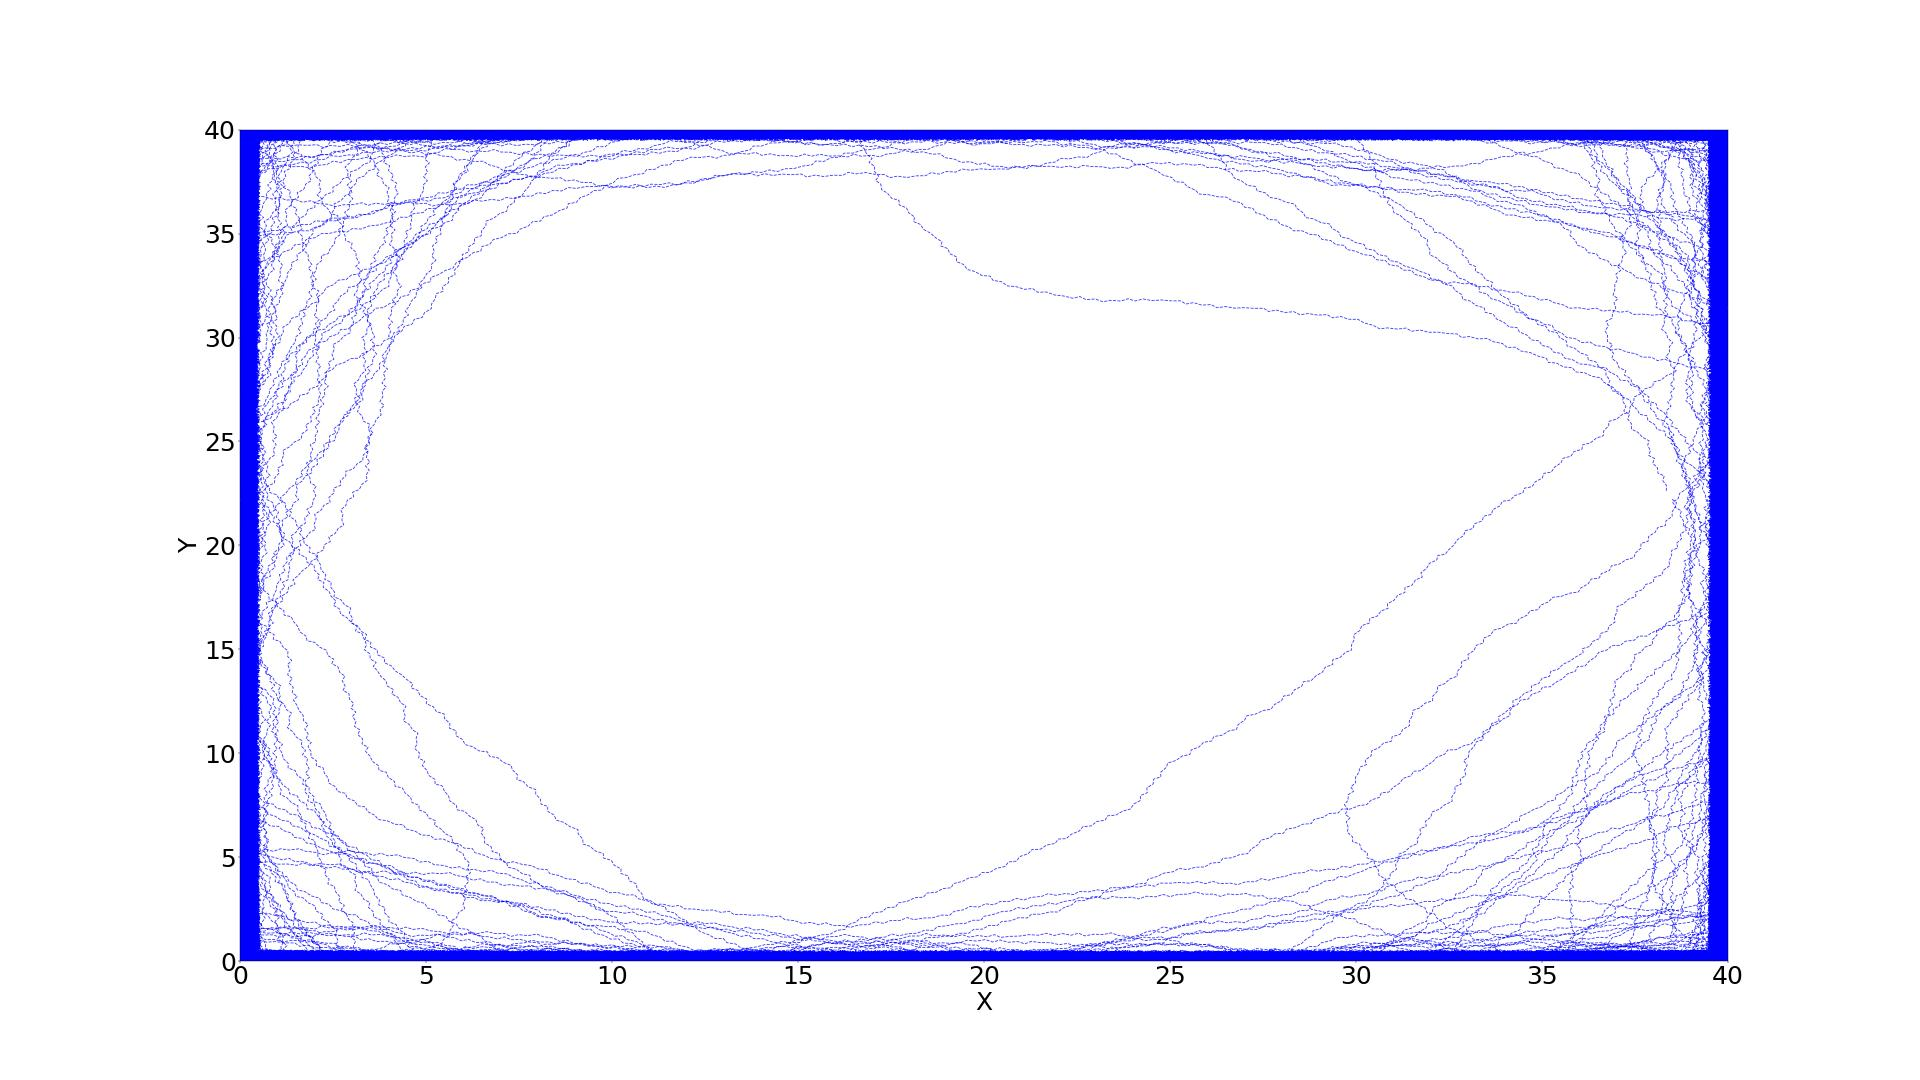
\includegraphics[width=\textwidth]{LateX images/log/steps/g2-1.6}
	\caption{Αριθμό βημάτων $10^6$ και ποσοστό κάλυψης $25.57$.}
	\label{f:g110}
\end{subfigure}
\hfill
\begin{subfigure}[b]{0.75\textwidth}
	\centering
	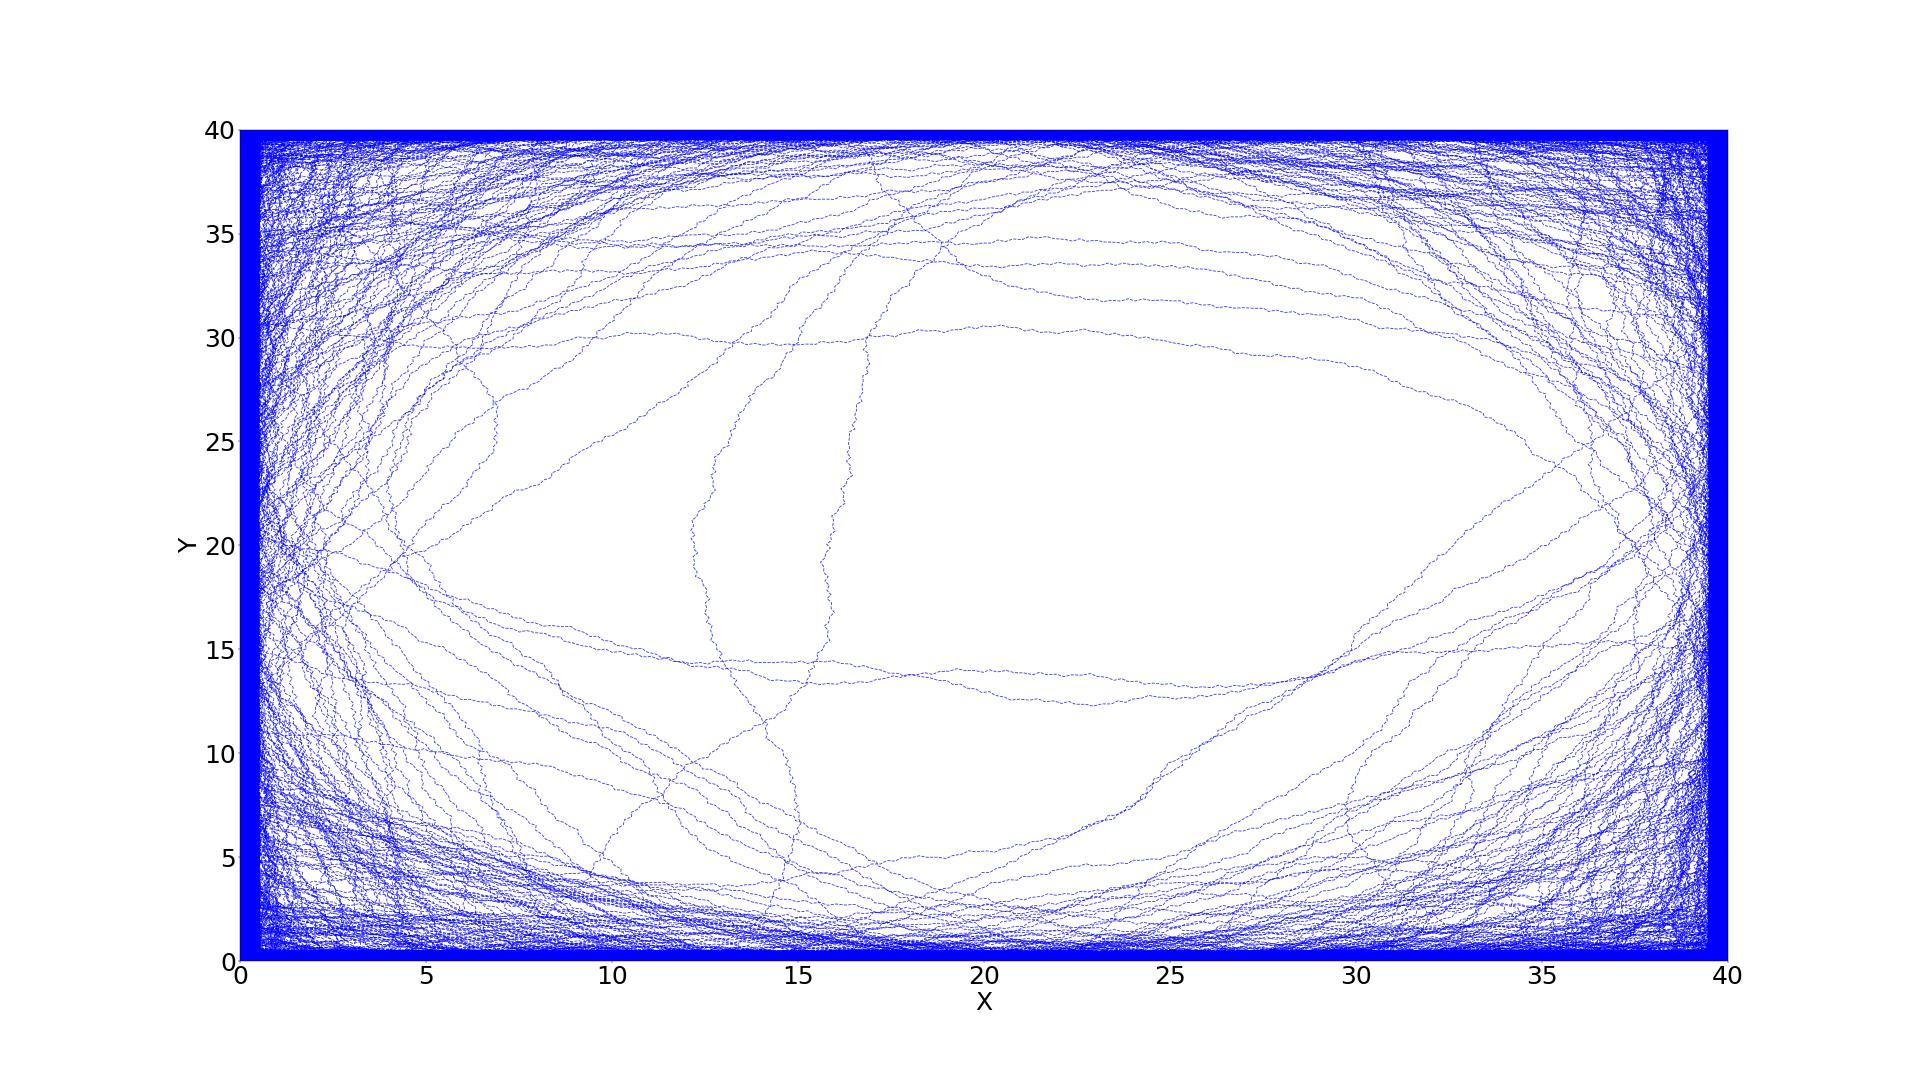
\includegraphics[width=\textwidth]{LateX images/log/steps/g1-1.6}
	\caption{Αριθμό βημάτων $5*10^6$ και ποσοστό κάλυψης $51.25$.}
	\label{f:g111}
\end{subfigure}
\hfill
\caption{Διαγράμματα διαδρομής ρομποτικού συστήματος για, $q = -1.6$, $k = 0.79$ :}
\end{figure}

\clearpage

\subsection{Για \emph{q = -1.9}}

Σύμφωνα με τα δεδομένα του πίνακα \ref{tab:abc15} κατασκευάστηκε διάγραμμα του αριθμού των βημάτων που εκτελεί το ρομπότ συναρτήσει του ποσοστού κάλυψης. Όπως φαίνεται στο Σχ. \ref{f:g112} η μεταβολή της συναρτησιακής αυτής σχέσης είναι κατά προσέγγιση εκθετική. Στα Σχ. \ref{f:g113}, \ref{f:g114}, \ref{f:g115} παρουσιάζονται τα διαγράμματα διαδρομής ρομποτικού συστήματος, για αριθμό βημάτων $10^4$, $5*10^4$ και $10^5$ αντίστοιχα.

\begin{table}[ht]
	\centering
	\caption{Συμπεριφορά του υπό μελέτη συστήματος για διαφορετικό αριθμό βημάτων και για $q = -1.9$, $k = 0.68$.}
	\begin{tabular}{l | l }
		Αριθμός Βημάτων & Ποσοστό Κάλυψης \\
		
		$10^4$ &  $15.125$ \\
		$5*10^4$ & $54.254$\\
		$7*10^4$&  $64.840$ \\
		$10^5$ & $81.082$\\
		$5*10^5$& $99.98$\\
		$10^6$& $100$\\
		
	\end{tabular}	
	\label{tab:abc15}
\end{table}

\begin{figure}[ht]
	\centering
	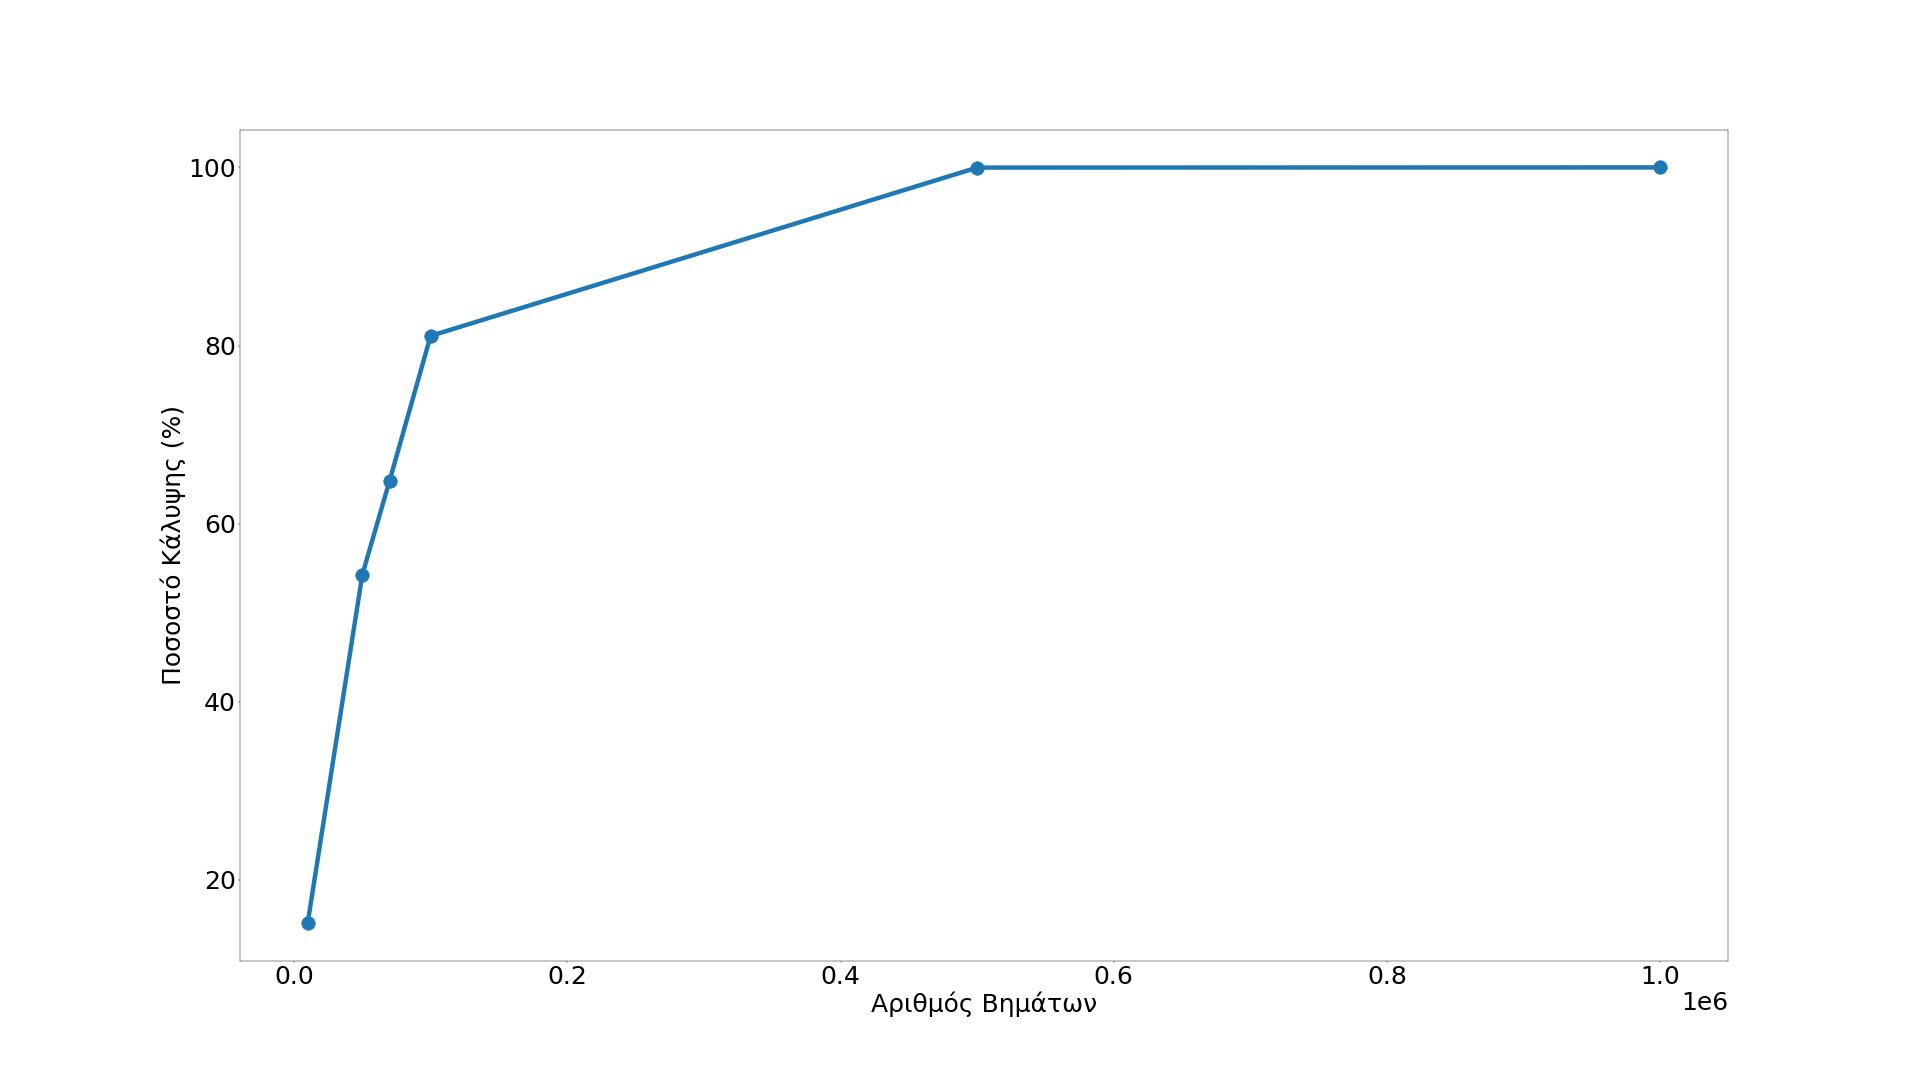
\includegraphics[width=1\linewidth]{LateX images/log/steps/g2}
	\caption{Διάγραμμα μεταβολής του ποσοστού κάλυψης συναρτήσει του αριθμού βημάτων για $q = -1.9$ και $k= 0.68$.}
	\label{f:g112}	
\end{figure}

\begin{figure}[ht]
	\centering
	\begin{subfigure}[b]{0.75\textwidth}
		\centering
		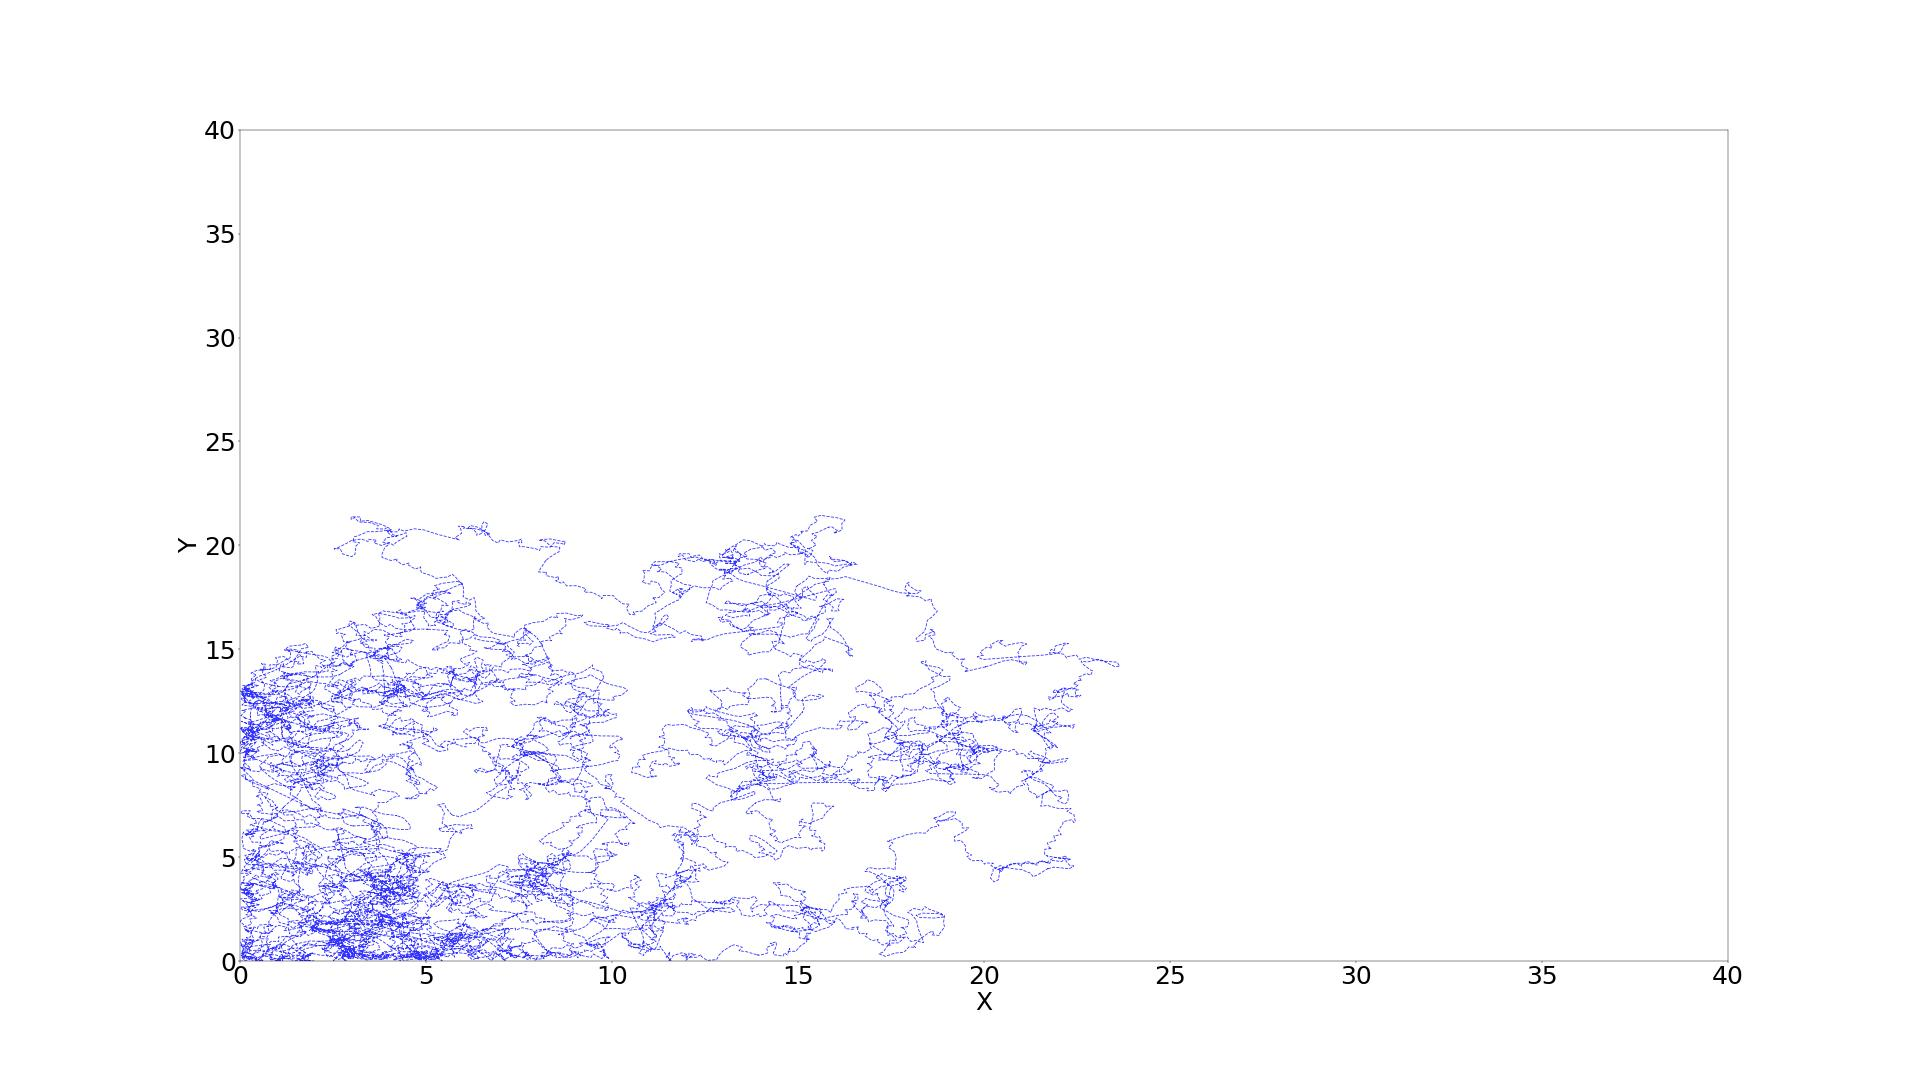
\includegraphics[width=\textwidth]{LateX images/log/steps/g1-1.9}
		\caption{Αριθμό βημάτων $10^4$ και ποσοστό κάλυψης $15.125$ .}
		\label{f:g113}
	\end{subfigure}
	\hfill
	\begin{subfigure}[b]{0.75\textwidth}
		\centering
		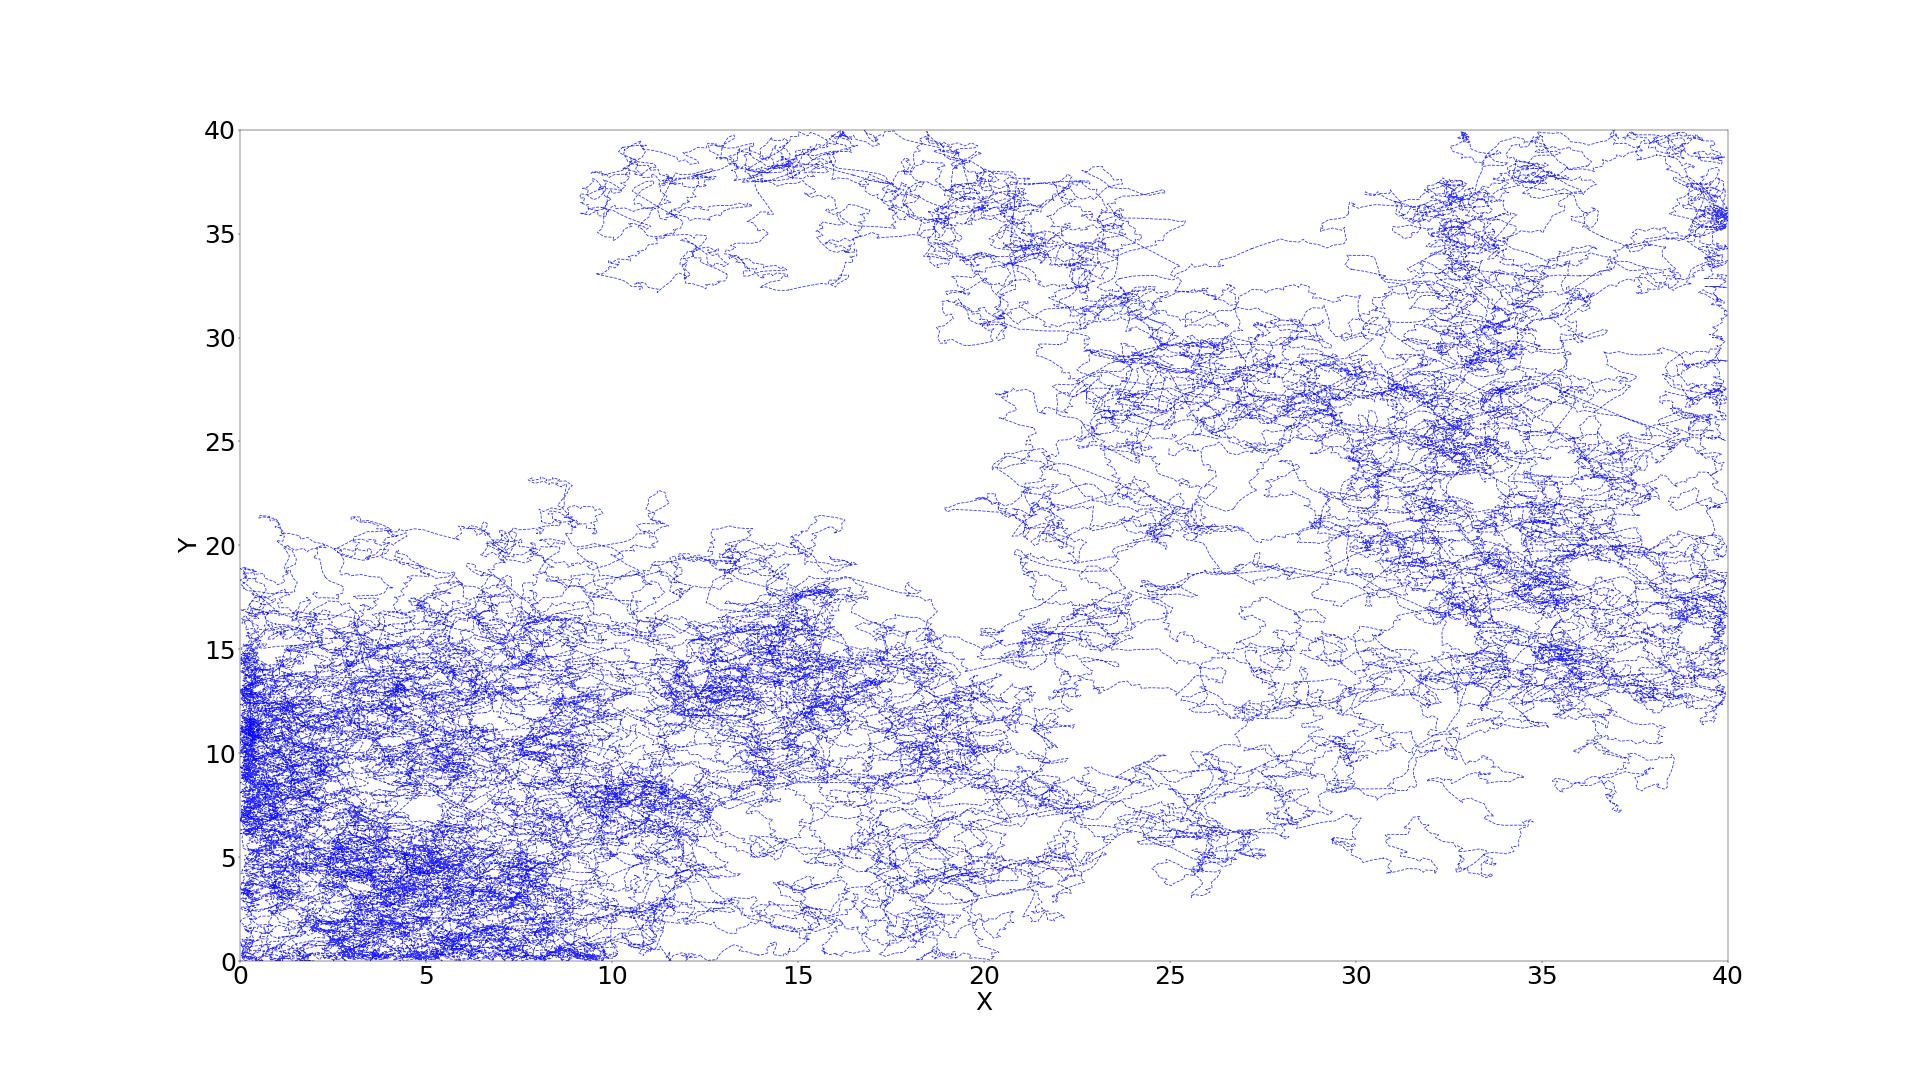
\includegraphics[width=\textwidth]{LateX images/log/steps/g2-1.9}
		\caption{Αριθμό βημάτων $5*10^4$ και ποσοστό κάλυψης $81.082$.}
		\label{f:g114}
	\end{subfigure}
	\hfill
	\begin{subfigure}[b]{0.75\textwidth}
		\centering
		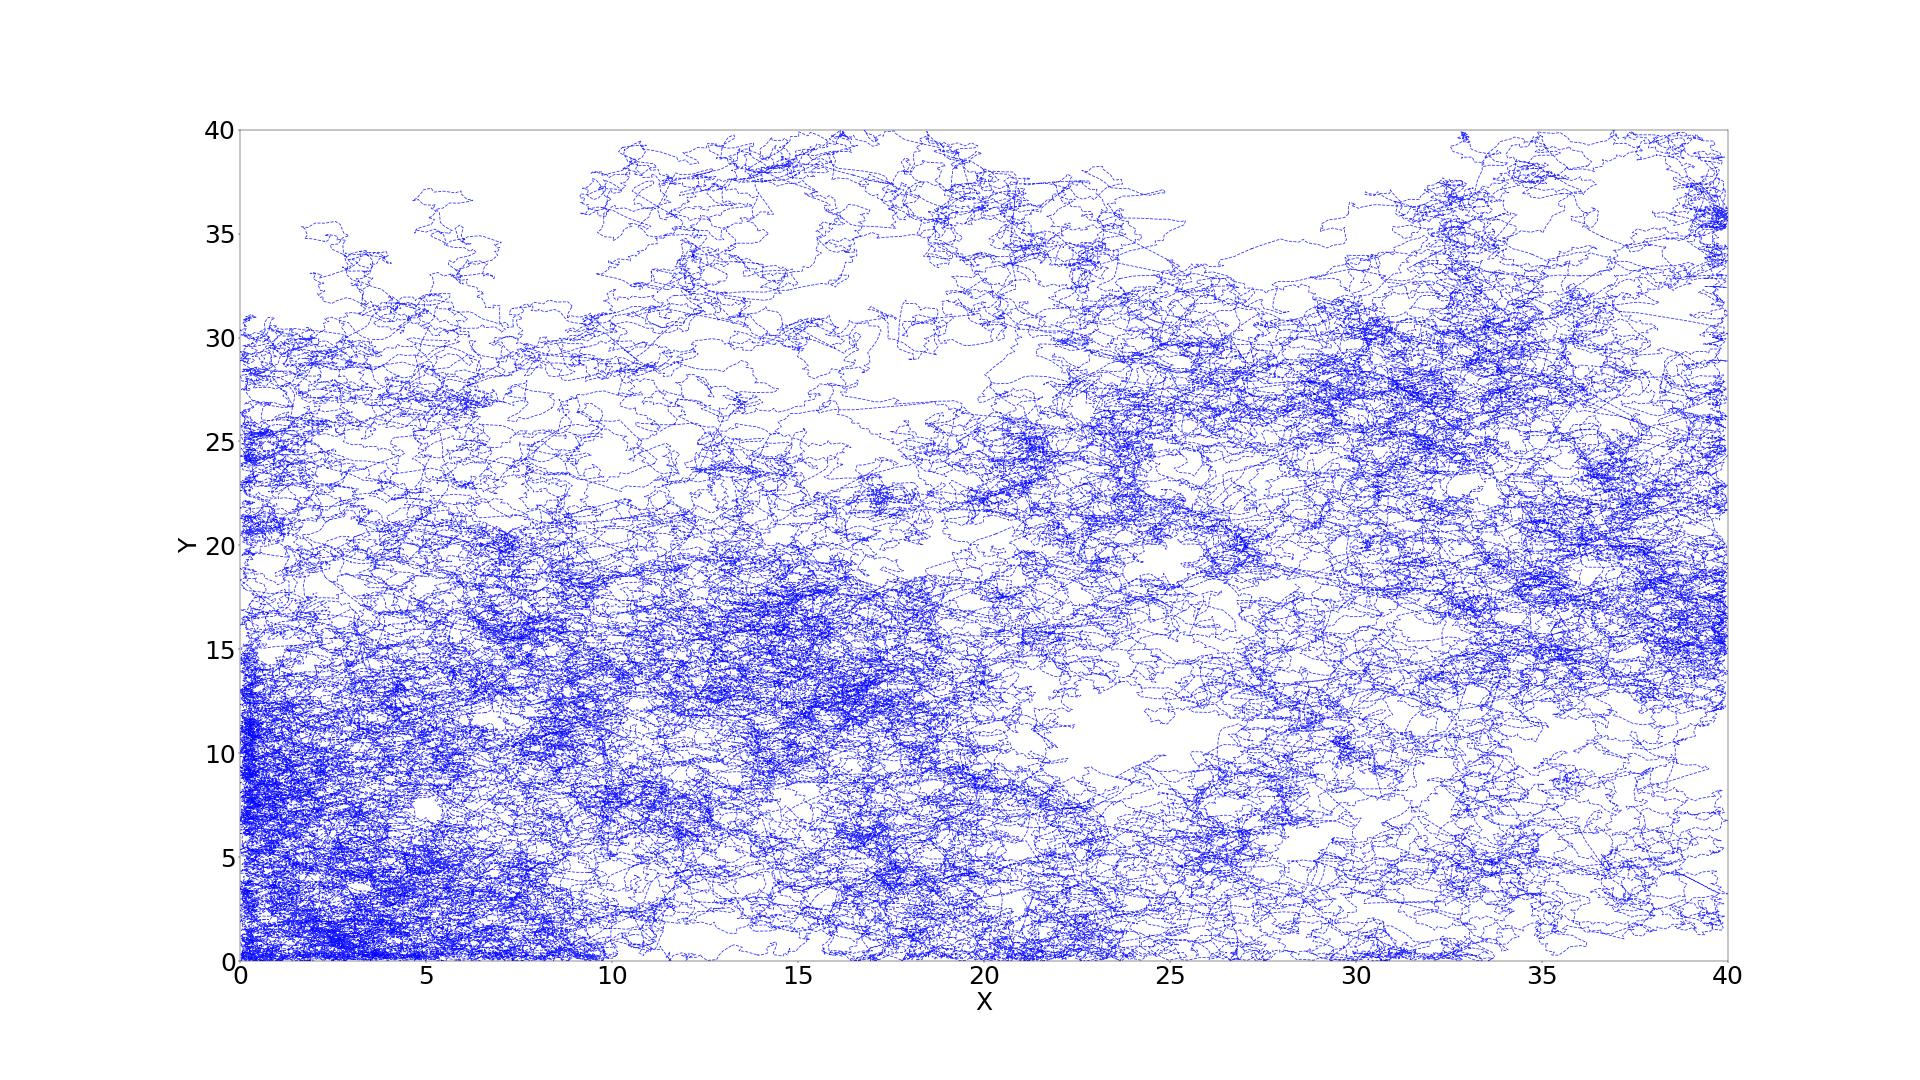
\includegraphics[width=\textwidth]{LateX images/log/steps/g4-1.9}
		\caption{Αριθμό βημάτων $10^5$ και ποσοστό κάλυψης $54.254$.}
		\label{f:g115}
	\end{subfigure}
	\hfill
	\caption{Διαγράμματα διαδρομής ρομποτικού συστήματος για, $q = -1.9$, $k = 0.68$ :}
\end{figure}
\clearpage

\section{Συμπεράσματα}

Από την παραπάνω μελέτη της συμπεριφοράς του ρομποτικού συστήματος,με βάση τις διάφορες τιμές των παραμέτρων της κίνησης, για συγκεκριμένες τιμές της παραμέτρου \emph{q} συμπαιρένουμε ότι η διαδρομή που ακολουθεί το ρομποτ είναι ευαίσθητη στην μεταβολή όλων των παραμέτρων. Οι τιμές των παραμέτρων που χρησιμοποιήθηκαν δεν αλλάξανε συμπεριφορά του συστήματος, δηλαδή βρισκόταν σε όλες τις περιπτώσεις στο χάος.Αυτό επιλέχθηκε ώστε να υπάρχει μία βάση στην μελέτη και τα αποτελέσματα να είναι συγκρίσιμα.
 
Συγκεκριμένα, η μεταβολή της παραμέτρου \emph{q} και της παραμέτρου διακλάδωσης \emph{k} στην παράγραφο \ref{sec:g1} προκαλούσε αισθητή αλλαγή στο ποσοστό κάλυψης της διαδρομής του ρομπότ ειδικά στις περιπτώσεις όπου μεταβαλλόταν το \emph{k} όπως στις παραγράφους \ref{par:g2}, \ref{par:g3}.

Aπό την άλλη η αλλαγή στις αρχικές συντεταγμένες $(Χ,Υ)$ της επιφάνειας που κινείται το ρομποτικό σύστημα, στην παράγραφο \ref{sec:g2} προκάλεσε ελάχιστη μεταβολή της καλυψιμότητας.

Επιπλέον, η αλλαγή στις αρχικές  συνθήκες $(x,y)$ στην παράγραφο \ref{sec:g3}, προκαλούσε τυχαίες μεταβολές στο ποσοστό κάλυψης του χωρου. Συνεπώς,δεν μπορεί να προκύψει κάποιο συγκεκριμένο αποτέλεσμα από τον έλεγχο της συγκεκριμένης παραμέτρου.

Τέλος, εκθετική αύξηση της καλυψιμότητας της επιφάνειας, προέκυπτε
από τις περιπτώσεις που αυξάναμε την παράμετρο διακριτοποίησης \emph{h} στην παράγραφο \ref{sec:g4} και όσο αυξανόταν ο αριθμός βημάτων που εκτελεί το ρομπότ σε μία διαδρομή, στην παράγραφο \ref{sec:g5}.

Οι συνδυασμοί των παραμέτρων που μπορούμε να πραγματοποιήσουμε είναι άπειροι, συνεπώς και οι διαδρομές, με τα αντίστοιχα ποσοστά κάλυψης του χώρου, που μπορεί να ακολουθήσει το ρομπότ στον χώρο.